\documentclass[twoside]{book}

% Packages required by doxygen
\usepackage{fixltx2e}
\usepackage{calc}
\usepackage{doxygen}
\usepackage[export]{adjustbox} % also loads graphicx
\usepackage{graphicx}
\usepackage[utf8]{inputenc}
\usepackage{makeidx}
\usepackage{multicol}
\usepackage{multirow}
\PassOptionsToPackage{warn}{textcomp}
\usepackage{textcomp}
\usepackage[nointegrals]{wasysym}
\usepackage[table]{xcolor}

% Font selection
\usepackage[T1]{fontenc}
\usepackage[scaled=.90]{helvet}
\usepackage{courier}
\usepackage{amssymb}
\usepackage{sectsty}
\renewcommand{\familydefault}{\sfdefault}
\allsectionsfont{%
  \fontseries{bc}\selectfont%
  \color{darkgray}%
}
\renewcommand{\DoxyLabelFont}{%
  \fontseries{bc}\selectfont%
  \color{darkgray}%
}
\newcommand{\+}{\discretionary{\mbox{\scriptsize$\hookleftarrow$}}{}{}}

% Page & text layout
\usepackage{geometry}
\geometry{%
  a4paper,%
  top=2.5cm,%
  bottom=2.5cm,%
  left=2.5cm,%
  right=2.5cm%
}
\tolerance=750
\hfuzz=15pt
\hbadness=750
\setlength{\emergencystretch}{15pt}
\setlength{\parindent}{0cm}
\setlength{\parskip}{3ex plus 2ex minus 2ex}
\makeatletter
\renewcommand{\paragraph}{%
  \@startsection{paragraph}{4}{0ex}{-1.0ex}{1.0ex}{%
    \normalfont\normalsize\bfseries\SS@parafont%
  }%
}
\renewcommand{\subparagraph}{%
  \@startsection{subparagraph}{5}{0ex}{-1.0ex}{1.0ex}{%
    \normalfont\normalsize\bfseries\SS@subparafont%
  }%
}
\makeatother

% Headers & footers
\usepackage{fancyhdr}
\pagestyle{fancyplain}
\fancyhead[LE]{\fancyplain{}{\bfseries\thepage}}
\fancyhead[CE]{\fancyplain{}{}}
\fancyhead[RE]{\fancyplain{}{\bfseries\leftmark}}
\fancyhead[LO]{\fancyplain{}{\bfseries\rightmark}}
\fancyhead[CO]{\fancyplain{}{}}
\fancyhead[RO]{\fancyplain{}{\bfseries\thepage}}
\fancyfoot[LE]{\fancyplain{}{}}
\fancyfoot[CE]{\fancyplain{}{}}
\fancyfoot[RE]{\fancyplain{}{\bfseries\scriptsize Generated by Doxygen }}
\fancyfoot[LO]{\fancyplain{}{\bfseries\scriptsize Generated by Doxygen }}
\fancyfoot[CO]{\fancyplain{}{}}
\fancyfoot[RO]{\fancyplain{}{}}
\renewcommand{\footrulewidth}{0.4pt}
\renewcommand{\chaptermark}[1]{%
  \markboth{#1}{}%
}
\renewcommand{\sectionmark}[1]{%
  \markright{\thesection\ #1}%
}

% Indices & bibliography
\usepackage{natbib}
\usepackage[titles]{tocloft}
\setcounter{tocdepth}{3}
\setcounter{secnumdepth}{5}
\makeindex

% Hyperlinks (required, but should be loaded last)
\usepackage{ifpdf}
\ifpdf
  \usepackage[pdftex,pagebackref=true]{hyperref}
\else
  \usepackage[ps2pdf,pagebackref=true]{hyperref}
\fi
\hypersetup{%
  colorlinks=true,%
  linkcolor=blue,%
  citecolor=blue,%
  unicode%
}

% Custom commands
\newcommand{\clearemptydoublepage}{%
  \newpage{\pagestyle{empty}\cleardoublepage}%
}

\usepackage{caption}
\captionsetup{labelsep=space,justification=centering,font={bf},singlelinecheck=off,skip=4pt,position=top}

%===== C O N T E N T S =====

\begin{document}

% Titlepage & ToC
\hypersetup{pageanchor=false,
             bookmarksnumbered=true,
             pdfencoding=unicode
            }
\pagenumbering{alph}
\begin{titlepage}
\vspace*{7cm}
\begin{center}%
{\Large chinet }\\
\vspace*{1cm}
{\large Generated by Doxygen 1.8.13}\\
\end{center}
\end{titlepage}
\clearemptydoublepage
\pagenumbering{roman}
\tableofcontents
\clearemptydoublepage
\pagenumbering{arabic}
\hypersetup{pageanchor=true}

%--- Begin generated contents ---
\chapter{chinet}
\label{index}\hypertarget{index}{}\input{index}
\chapter{Namespace Index}
\section{Namespace List}
Here is a list of all namespaces with brief descriptions\+:\begin{DoxyCompactList}
\item\contentsline{section}{\hyperlink{namespace_functions}{Functions} }{\pageref{namespace_functions}}{}
\item\contentsline{section}{\hyperlink{namespace_pda_functions}{Pda\+Functions} }{\pageref{namespace_pda_functions}}{}
\end{DoxyCompactList}

\chapter{Hierarchical Index}
\section{Class Hierarchy}
This inheritance list is sorted roughly, but not completely, alphabetically\+:\begin{DoxyCompactList}
\item \contentsline{section}{Curve}{\pageref{class_curve}}{}
\begin{DoxyCompactList}
\item \contentsline{section}{Exponential\+Decay}{\pageref{class_exponential_decay}}{}
\end{DoxyCompactList}
\item \contentsline{section}{Port\+:\+:get\+\_\+value}{\pageref{class_port_1_1get__value}}{}
\item \contentsline{section}{Mongo\+Object}{\pageref{class_mongo_object}}{}
\begin{DoxyCompactList}
\item \contentsline{section}{Base\+Port}{\pageref{class_base_port}}{}
\begin{DoxyCompactList}
\item \contentsline{section}{Value\+Port}{\pageref{class_value_port}}{}
\begin{DoxyCompactList}
\item \contentsline{section}{Port}{\pageref{class_port}}{}
\end{DoxyCompactList}
\end{DoxyCompactList}
\item \contentsline{section}{Node}{\pageref{class_node}}{}
\item \contentsline{section}{Session}{\pageref{class_session}}{}
\end{DoxyCompactList}
\item \contentsline{section}{Node\+Callback}{\pageref{class_node_callback}}{}
\item \contentsline{section}{Pda}{\pageref{class_pda}}{}
\item \contentsline{section}{Port\+Links$<$ T $>$}{\pageref{class_port_links}}{}
\item \contentsline{section}{Port\+Links$<$ double $>$}{\pageref{class_port_links}}{}
\end{DoxyCompactList}

\chapter{Class Index}
\section{Class List}
Here are the classes, structs, unions and interfaces with brief descriptions\+:\begin{DoxyCompactList}
\item\contentsline{section}{\hyperlink{class_curve}{Curve} }{\pageref{class_curve}}{}
\item\contentsline{section}{\hyperlink{class_decay}{Decay} }{\pageref{class_decay}}{}
\item\contentsline{section}{\hyperlink{class_mongo_object}{Mongo\+Object} \\*Connects the instance of database }{\pageref{class_mongo_object}}{}
\item\contentsline{section}{\hyperlink{class_node}{Node} }{\pageref{class_node}}{}
\item\contentsline{section}{\hyperlink{class_node_callback}{Node\+Callback} }{\pageref{class_node_callback}}{}
\item\contentsline{section}{\hyperlink{class_pda}{Pda} }{\pageref{class_pda}}{}
\item\contentsline{section}{\hyperlink{class_port}{Port} }{\pageref{class_port}}{}
\item\contentsline{section}{\hyperlink{class_session}{Session} }{\pageref{class_session}}{}
\end{DoxyCompactList}

\chapter{File Index}
\section{File List}
Here is a list of all files with brief descriptions\+:\begin{DoxyCompactList}
\item\contentsline{section}{include/\hyperlink{_curve_8h}{Curve.\+h} }{\pageref{_curve_8h}}{}
\item\contentsline{section}{include/\hyperlink{_exponential_decay_8h}{Exponential\+Decay.\+h} }{\pageref{_exponential_decay_8h}}{}
\item\contentsline{section}{include/\hyperlink{_functions_8h}{Functions.\+h} }{\pageref{_functions_8h}}{}
\item\contentsline{section}{include/\hyperlink{_mongo_object_8h}{Mongo\+Object.\+h} }{\pageref{_mongo_object_8h}}{}
\item\contentsline{section}{include/\hyperlink{_node_8h}{Node.\+h} }{\pageref{_node_8h}}{}
\item\contentsline{section}{include/\hyperlink{_node_callback_8h}{Node\+Callback.\+h} }{\pageref{_node_callback_8h}}{}
\item\contentsline{section}{include/\hyperlink{_pda_8h}{Pda.\+h} }{\pageref{_pda_8h}}{}
\item\contentsline{section}{include/\hyperlink{_port_8h}{Port.\+h} }{\pageref{_port_8h}}{}
\item\contentsline{section}{include/\hyperlink{_port_links_8h}{Port\+Links.\+h} }{\pageref{_port_links_8h}}{}
\item\contentsline{section}{include/\hyperlink{_session_8h}{Session.\+h} }{\pageref{_session_8h}}{}
\end{DoxyCompactList}

\chapter{Namespace Documentation}
\hypertarget{namespace_functions}{}\section{Functions Namespace Reference}
\label{namespace_functions}\index{Functions@{Functions}}
\subsection*{Functions}
\begin{DoxyCompactItemize}
\item 
void \hyperlink{namespace_functions_a9327d93975ced0eda3d86e7cc0eaa2ce}{shift} (double value, std\+::vector$<$ double $>$ \&x)
\item 
void \hyperlink{namespace_functions_a3f9558335e568ef96875e356712737d5}{roll} (int value, std\+::vector$<$ double $>$ \&y)
\item 
void \hyperlink{namespace_functions_a2f190c8d48a79957846060e91638daf0}{copy\+\_\+vector\+\_\+to\+\_\+array} (std\+::vector$<$ double $>$ \&v, double $\ast$$\ast$out, int $\ast$nout)
\item 
void \hyperlink{namespace_functions_a89a9951b3cfcc5c8e51d53a95361a722}{copy\+\_\+vector\+\_\+to\+\_\+array} (std\+::vector$<$ double $>$ \&v, double $\ast$out, int nout)
\item 
void \hyperlink{namespace_functions_a680d81633db9ad1074e4053e49aab936}{copy\+\_\+array\+\_\+to\+\_\+vector} (double $\ast$in, int nin, std\+::vector$<$ double $>$ \&v)
\item 
void \hyperlink{namespace_functions_a8e230f278da41398c7475369f9dcf100}{copy\+\_\+two\+\_\+vectors\+\_\+to\+\_\+interleaved\+\_\+array} (std\+::vector$<$ double $>$ \&v1, std\+::vector$<$ double $>$ \&v2, double $\ast$$\ast$out, int $\ast$nout)
\item 
void \hyperlink{namespace_functions_a2ba36946f1e5125d51a9970f3b8300ea}{convolve\+\_\+sum\+\_\+of\+\_\+exponentials} (double $\ast$out, int n\+\_\+out, const double $\ast$lifetime\+\_\+spectrum, int n\+\_\+lifetime\+\_\+spectrum, const double $\ast$irf, int n\+\_\+irf, int convolution\+\_\+stop, double dt)
\item 
void \hyperlink{namespace_functions_ae70edf0473b6bebe1325e50b3971ef22}{convolve\+\_\+sum\+\_\+of\+\_\+exponentials\+\_\+periodic} (double $\ast$out, int n\+\_\+out, const double $\ast$lifetime, int n\+\_\+lifetimes, const double $\ast$irf, int n\+\_\+irf, int start, int stop, double dt, double period)
\item 
std\+::vector$<$ double $>$ \hyperlink{namespace_functions_af4928f5c5dcc2034838ac8cd3c1ad2a4}{diff} (std\+::vector$<$ double $>$ v)
\item 
uint64\+\_\+t \hyperlink{namespace_functions_a0f3325eb8b88e73ff76e558290d3b346}{get\+\_\+time} ()
\item 
void \hyperlink{namespace_functions_ae254385436f80c3069a0a2f74df4d741}{add\+\_\+documents} (bson\+\_\+t $\ast$src, bson\+\_\+t $\ast$dst, std\+::vector$<$ std\+::string $>$ skip)
\item 
bool \hyperlink{namespace_functions_a7948d719f3f38161f1fe1572072224bc}{bson\+\_\+iter\+\_\+skip} (bson\+\_\+iter\+\_\+t $\ast$iter, std\+::vector$<$ std\+::string $>$ $\ast$skip)
\end{DoxyCompactItemize}


\subsection{Function Documentation}
\mbox{\Hypertarget{namespace_functions_ae254385436f80c3069a0a2f74df4d741}\label{namespace_functions_ae254385436f80c3069a0a2f74df4d741}} 
\index{Functions@{Functions}!add\+\_\+documents@{add\+\_\+documents}}
\index{add\+\_\+documents@{add\+\_\+documents}!Functions@{Functions}}
\subsubsection{\texorpdfstring{add\+\_\+documents()}{add\_documents()}}
{\footnotesize\ttfamily void Functions\+::add\+\_\+documents (\begin{DoxyParamCaption}\item[{bson\+\_\+t $\ast$}]{src,  }\item[{bson\+\_\+t $\ast$}]{dst,  }\item[{std\+::vector$<$ std\+::string $>$}]{skip }\end{DoxyParamCaption})}

Adds the content in the bson\+\_\+t document src to the document dst omitting the keys provided by the vector skip. \mbox{\Hypertarget{namespace_functions_a7948d719f3f38161f1fe1572072224bc}\label{namespace_functions_a7948d719f3f38161f1fe1572072224bc}} 
\index{Functions@{Functions}!bson\+\_\+iter\+\_\+skip@{bson\+\_\+iter\+\_\+skip}}
\index{bson\+\_\+iter\+\_\+skip@{bson\+\_\+iter\+\_\+skip}!Functions@{Functions}}
\subsubsection{\texorpdfstring{bson\+\_\+iter\+\_\+skip()}{bson\_iter\_skip()}}
{\footnotesize\ttfamily bool Functions\+::bson\+\_\+iter\+\_\+skip (\begin{DoxyParamCaption}\item[{bson\+\_\+iter\+\_\+t $\ast$}]{iter,  }\item[{std\+::vector$<$ std\+::string $>$ $\ast$}]{skip }\end{DoxyParamCaption})}

Returns true if the key associated to 
\begin{DoxyParams}{Parameters}
{\em iter} & is in the list of vectors \\
\hline
{\em skip} & \\
\hline
{\em iter} & pointer to a bson\+\_\+iter\+\_\+t \\
\hline
{\em skip} & vector of strings containing keys that are skipped by iter \\
\hline
\end{DoxyParams}
\mbox{\Hypertarget{namespace_functions_a2ba36946f1e5125d51a9970f3b8300ea}\label{namespace_functions_a2ba36946f1e5125d51a9970f3b8300ea}} 
\index{Functions@{Functions}!convolve\+\_\+sum\+\_\+of\+\_\+exponentials@{convolve\+\_\+sum\+\_\+of\+\_\+exponentials}}
\index{convolve\+\_\+sum\+\_\+of\+\_\+exponentials@{convolve\+\_\+sum\+\_\+of\+\_\+exponentials}!Functions@{Functions}}
\subsubsection{\texorpdfstring{convolve\+\_\+sum\+\_\+of\+\_\+exponentials()}{convolve\_sum\_of\_exponentials()}}
{\footnotesize\ttfamily void Functions\+::convolve\+\_\+sum\+\_\+of\+\_\+exponentials (\begin{DoxyParamCaption}\item[{double $\ast$}]{out,  }\item[{int}]{n\+\_\+out,  }\item[{const double $\ast$}]{lifetime\+\_\+spectrum,  }\item[{int}]{n\+\_\+lifetime\+\_\+spectrum,  }\item[{const double $\ast$}]{irf,  }\item[{int}]{n\+\_\+irf,  }\item[{int}]{convolution\+\_\+stop,  }\item[{double}]{dt }\end{DoxyParamCaption})}

This function convolves a sum of exponential decays with an instrument response function (I\+RF)

The sum of exponential decays is passed by the lifetime array 
\begin{DoxyParams}{Parameters}
{\em lifetime\+\_\+spectrum} & that contains the amplitudes and the corresponding fluorescence lifetimes in an interleaved array (amplitude\+\_\+1, lifetime\+\_\+1, amplitude\+\_\+2, lifetime\+\_\+2, ...). The instrument response function is passed by the array \\
\hline
{\em irf.} & The I\+RF and the and the sum of exponential decays are convolved up to the index \\
\hline
{\em convolution\+\_\+stop.} & In this convolution, the time axis is uniform an linear with a time interval specified by the parameter \\
\hline
{\em dt.} & \\
\hline
{\em out} & The array to which the convoluted decay is written to \\
\hline
{\em n\+\_\+out} & The number of elements in the output array \\
\hline
{\em lifetime\+\_\+spectrum} & The array containing the fluorescence lifetimes and the amplitudes \\
\hline
{\em n\+\_\+lifetime\+\_\+spectrum} & The number of fluorescence lifetimes \\
\hline
{\em irf} & The array containing the instrument response function \\
\hline
{\em n\+\_\+irf} & The number of elements of the instrument response function \\
\hline
{\em convolution\+\_\+stop} & The stop of the convolution \\
\hline
{\em dt} & The time resolution \\
\hline
\end{DoxyParams}
\mbox{\Hypertarget{namespace_functions_ae70edf0473b6bebe1325e50b3971ef22}\label{namespace_functions_ae70edf0473b6bebe1325e50b3971ef22}} 
\index{Functions@{Functions}!convolve\+\_\+sum\+\_\+of\+\_\+exponentials\+\_\+periodic@{convolve\+\_\+sum\+\_\+of\+\_\+exponentials\+\_\+periodic}}
\index{convolve\+\_\+sum\+\_\+of\+\_\+exponentials\+\_\+periodic@{convolve\+\_\+sum\+\_\+of\+\_\+exponentials\+\_\+periodic}!Functions@{Functions}}
\subsubsection{\texorpdfstring{convolve\+\_\+sum\+\_\+of\+\_\+exponentials\+\_\+periodic()}{convolve\_sum\_of\_exponentials\_periodic()}}
{\footnotesize\ttfamily void Functions\+::convolve\+\_\+sum\+\_\+of\+\_\+exponentials\+\_\+periodic (\begin{DoxyParamCaption}\item[{double $\ast$}]{out,  }\item[{int}]{n\+\_\+out,  }\item[{const double $\ast$}]{lifetime,  }\item[{int}]{n\+\_\+lifetimes,  }\item[{const double $\ast$}]{irf,  }\item[{int}]{n\+\_\+irf,  }\item[{int}]{start,  }\item[{int}]{stop,  }\item[{double}]{dt,  }\item[{double}]{period }\end{DoxyParamCaption})}

This function convolves a sum of exponential decays with an instrument response function (I\+RF)

The sum of exponential decays is passed by the lifetime array 
\begin{DoxyParams}{Parameters}
{\em lifetime} & that contains the amplitudes and the corresponding fluorescence lifetimes in an interleaved array (amplitude\+\_\+1, lifetime\+\_\+1, amplitude\+\_\+2, lifetime\+\_\+2, ...). The instrument response function is passed by the array \\
\hline
{\em irf.} & The I\+RF and the and the sum of exponential decays are convolved up to the index \\
\hline
{\em convolution\+\_\+stop.} & In this convolution, the time axis is uniform an linear with a time interval specified by the parameter \\
\hline
{\em dt.} & \\
\hline
{\em out} & The array to which the convoluted decay is written to \\
\hline
{\em n\+\_\+out} & The number of elements in the output array \\
\hline
{\em lifetime} & The array containing the fluorescence lifetimes and the amplitudes \\
\hline
{\em n\+\_\+lifetimes} & The number of fluorescence lifetimes \\
\hline
{\em irf} & The array containing the instrument response function \\
\hline
{\em n\+\_\+irf} & The number of elements of the instrument response function \\
\hline
{\em start} & The start index of the convolution \\
\hline
{\em stop} & The stop index of the convolution \\
\hline
{\em dt} & The time resolution \\
\hline
{\em period} & The time between repeated excitation intervals \\
\hline
\end{DoxyParams}
\mbox{\Hypertarget{namespace_functions_a680d81633db9ad1074e4053e49aab936}\label{namespace_functions_a680d81633db9ad1074e4053e49aab936}} 
\index{Functions@{Functions}!copy\+\_\+array\+\_\+to\+\_\+vector@{copy\+\_\+array\+\_\+to\+\_\+vector}}
\index{copy\+\_\+array\+\_\+to\+\_\+vector@{copy\+\_\+array\+\_\+to\+\_\+vector}!Functions@{Functions}}
\subsubsection{\texorpdfstring{copy\+\_\+array\+\_\+to\+\_\+vector()}{copy\_array\_to\_vector()}}
{\footnotesize\ttfamily void Functions\+::copy\+\_\+array\+\_\+to\+\_\+vector (\begin{DoxyParamCaption}\item[{double $\ast$}]{in,  }\item[{int}]{nin,  }\item[{std\+::vector$<$ double $>$ \&}]{v }\end{DoxyParamCaption})}


\begin{DoxyParams}{Parameters}
{\em in} & \\
\hline
{\em nin} & \\
\hline
{\em v} & \\
\hline
\end{DoxyParams}
\mbox{\Hypertarget{namespace_functions_a8e230f278da41398c7475369f9dcf100}\label{namespace_functions_a8e230f278da41398c7475369f9dcf100}} 
\index{Functions@{Functions}!copy\+\_\+two\+\_\+vectors\+\_\+to\+\_\+interleaved\+\_\+array@{copy\+\_\+two\+\_\+vectors\+\_\+to\+\_\+interleaved\+\_\+array}}
\index{copy\+\_\+two\+\_\+vectors\+\_\+to\+\_\+interleaved\+\_\+array@{copy\+\_\+two\+\_\+vectors\+\_\+to\+\_\+interleaved\+\_\+array}!Functions@{Functions}}
\subsubsection{\texorpdfstring{copy\+\_\+two\+\_\+vectors\+\_\+to\+\_\+interleaved\+\_\+array()}{copy\_two\_vectors\_to\_interleaved\_array()}}
{\footnotesize\ttfamily void Functions\+::copy\+\_\+two\+\_\+vectors\+\_\+to\+\_\+interleaved\+\_\+array (\begin{DoxyParamCaption}\item[{std\+::vector$<$ double $>$ \&}]{v1,  }\item[{std\+::vector$<$ double $>$ \&}]{v2,  }\item[{double $\ast$$\ast$}]{out,  }\item[{int $\ast$}]{nout }\end{DoxyParamCaption})}

This function copies two vectors of equal size to an interleaved array


\begin{DoxyParams}{Parameters}
{\em v1} & \\
\hline
{\em v2} & \\
\hline
{\em out} & \\
\hline
{\em nout} & \\
\hline
\end{DoxyParams}
\mbox{\Hypertarget{namespace_functions_a2f190c8d48a79957846060e91638daf0}\label{namespace_functions_a2f190c8d48a79957846060e91638daf0}} 
\index{Functions@{Functions}!copy\+\_\+vector\+\_\+to\+\_\+array@{copy\+\_\+vector\+\_\+to\+\_\+array}}
\index{copy\+\_\+vector\+\_\+to\+\_\+array@{copy\+\_\+vector\+\_\+to\+\_\+array}!Functions@{Functions}}
\subsubsection{\texorpdfstring{copy\+\_\+vector\+\_\+to\+\_\+array()}{copy\_vector\_to\_array()}\hspace{0.1cm}{\footnotesize\ttfamily [1/2]}}
{\footnotesize\ttfamily void Functions\+::copy\+\_\+vector\+\_\+to\+\_\+array (\begin{DoxyParamCaption}\item[{std\+::vector$<$ double $>$ \&}]{v,  }\item[{double $\ast$$\ast$}]{out,  }\item[{int $\ast$}]{nout }\end{DoxyParamCaption})}

Allocates memory on a pointer to an array and copies the content of a vector to the newly allocated memory.

This function is mainly used for numpy array S\+W\+I\+Gs


\begin{DoxyParams}{Parameters}
{\em v} & \\
\hline
{\em out} & \\
\hline
{\em nout} & \\
\hline
\end{DoxyParams}
\mbox{\Hypertarget{namespace_functions_a89a9951b3cfcc5c8e51d53a95361a722}\label{namespace_functions_a89a9951b3cfcc5c8e51d53a95361a722}} 
\index{Functions@{Functions}!copy\+\_\+vector\+\_\+to\+\_\+array@{copy\+\_\+vector\+\_\+to\+\_\+array}}
\index{copy\+\_\+vector\+\_\+to\+\_\+array@{copy\+\_\+vector\+\_\+to\+\_\+array}!Functions@{Functions}}
\subsubsection{\texorpdfstring{copy\+\_\+vector\+\_\+to\+\_\+array()}{copy\_vector\_to\_array()}\hspace{0.1cm}{\footnotesize\ttfamily [2/2]}}
{\footnotesize\ttfamily void Functions\+::copy\+\_\+vector\+\_\+to\+\_\+array (\begin{DoxyParamCaption}\item[{std\+::vector$<$ double $>$ \&}]{v,  }\item[{double $\ast$}]{out,  }\item[{int}]{nout }\end{DoxyParamCaption})}

Copy an array and copies the content of a vector to already allocated memory.

This function is mainly used for numpy array S\+W\+I\+Gs


\begin{DoxyParams}{Parameters}
{\em v} & \\
\hline
{\em out} & \\
\hline
{\em nout} & \\
\hline
\end{DoxyParams}
\mbox{\Hypertarget{namespace_functions_af4928f5c5dcc2034838ac8cd3c1ad2a4}\label{namespace_functions_af4928f5c5dcc2034838ac8cd3c1ad2a4}} 
\index{Functions@{Functions}!diff@{diff}}
\index{diff@{diff}!Functions@{Functions}}
\subsubsection{\texorpdfstring{diff()}{diff()}}
{\footnotesize\ttfamily std\+::vector$<$double$>$ Functions\+::diff (\begin{DoxyParamCaption}\item[{std\+::vector$<$ double $>$}]{v }\end{DoxyParamCaption})}

Calculates the discrete difference for an vector


\begin{DoxyParams}{Parameters}
{\em v} & \\
\hline
\end{DoxyParams}
\begin{DoxyReturn}{Returns}

\end{DoxyReturn}
\mbox{\Hypertarget{namespace_functions_a0f3325eb8b88e73ff76e558290d3b346}\label{namespace_functions_a0f3325eb8b88e73ff76e558290d3b346}} 
\index{Functions@{Functions}!get\+\_\+time@{get\+\_\+time}}
\index{get\+\_\+time@{get\+\_\+time}!Functions@{Functions}}
\subsubsection{\texorpdfstring{get\+\_\+time()}{get\_time()}}
{\footnotesize\ttfamily uint64\+\_\+t Functions\+::get\+\_\+time (\begin{DoxyParamCaption}{ }\end{DoxyParamCaption})}

Returns the current time in milliseconds as a uint64 \begin{DoxyReturn}{Returns}

\end{DoxyReturn}
\mbox{\Hypertarget{namespace_functions_a3f9558335e568ef96875e356712737d5}\label{namespace_functions_a3f9558335e568ef96875e356712737d5}} 
\index{Functions@{Functions}!roll@{roll}}
\index{roll@{roll}!Functions@{Functions}}
\subsubsection{\texorpdfstring{roll()}{roll()}}
{\footnotesize\ttfamily void Functions\+::roll (\begin{DoxyParamCaption}\item[{int}]{value,  }\item[{std\+::vector$<$ double $>$ \&}]{y }\end{DoxyParamCaption})}

Rolls a vector by an integer


\begin{DoxyParams}{Parameters}
{\em value} & \\
\hline
{\em y} & \\
\hline
\end{DoxyParams}
\mbox{\Hypertarget{namespace_functions_a9327d93975ced0eda3d86e7cc0eaa2ce}\label{namespace_functions_a9327d93975ced0eda3d86e7cc0eaa2ce}} 
\index{Functions@{Functions}!shift@{shift}}
\index{shift@{shift}!Functions@{Functions}}
\subsubsection{\texorpdfstring{shift()}{shift()}}
{\footnotesize\ttfamily void Functions\+::shift (\begin{DoxyParamCaption}\item[{double}]{value,  }\item[{std\+::vector$<$ double $>$ \&}]{x }\end{DoxyParamCaption})}

Shifts a vector by a floating number.

This function shifts the y-\/axis and consider non-\/integer values by determining the integer part of the shift and the floating part of the shift value, e.\+g., for the shift 4.\+66 the integer part is 4 and the floating part is 0.\+66. Next the array is shifted by the integer part and a copy of the array is shifted by the integer part + 1. Finally, the weighted sum of the both arrays is calculated. 
\begin{DoxyParams}{Parameters}
{\em value} & \\
\hline
{\em x} & \\
\hline
\end{DoxyParams}

\hypertarget{namespace_pda_functions}{}\section{Pda\+Functions Namespace Reference}
\label{namespace_pda_functions}\index{Pda\+Functions@{Pda\+Functions}}
\subsection*{Functions}
\begin{DoxyCompactItemize}
\item 
void \hyperlink{namespace_pda_functions_a050993b2b90ecebe38776340834e0b50}{sgsr\+\_\+pN} (double $\ast$Sg\+Sr, double $\ast$pN, unsigned int Nmax, double Bg, double Br, double pg\+\_\+theor)
\item 
void \hyperlink{namespace_pda_functions_aa77615bc27d7b196fdbe50429ceadb86}{sgsr\+\_\+pF} (double $\ast$Sg\+Sr, double $\ast$pF, unsigned int Nmax, double Bg, double Br, double pg\+\_\+theor)
\item 
void \hyperlink{namespace_pda_functions_a38a72930ebb94ebee941a82cec608447}{sgsr\+\_\+p\+N\+\_\+manypg} (double $\ast$Sg\+Sr, double $\ast$pN, unsigned int Nmax, double Bg, double Br, unsigned int N\+\_\+pg, double $\ast$pg\+\_\+theor, double $\ast$a)
\item 
void \hyperlink{namespace_pda_functions_ac8c00ed27b7bfb24e099f98cfb9e5fba}{sgsr\+\_\+p\+F\+\_\+manypg} (double $\ast$Sg\+Sr, double $\ast$pF, unsigned int Nmax, double Bg, double Br, unsigned int N\+\_\+pg, double $\ast$pg\+\_\+theor, double $\ast$a)
\item 
void \hyperlink{namespace_pda_functions_afc3779dee6ad3e7d4a6f3c929ac0e160}{sgsr\+\_\+manypF} (double $\ast$, double $\ast$, unsigned int, double, double, unsigned int, double $\ast$, double $\ast$)
\item 
void \hyperlink{namespace_pda_functions_aaf576da99282a2a2695d3b216c3ed697}{conv\+\_\+pF} (double $\ast$Sg\+Sr, double $\ast$Fg\+Fr, unsigned int Nmax, double Bg, double Br)
\item 
void \hyperlink{namespace_pda_functions_a595a8233f39ec5db40e35c7de69dc019}{conv\+\_\+pN} (double $\ast$Sg\+Sr, double $\ast$Fg\+Fr, unsigned int Nmax, double Bg, double Br, double $\ast$pN)
\item 
void \hyperlink{namespace_pda_functions_ac9409faa9ab0ab98c2a659bcd5fa3071}{poisson\+\_\+0toN} (double $\ast$return\+\_\+p, double lambda, unsigned int return\+\_\+dim)
\item 
void \hyperlink{namespace_pda_functions_ab0ca4731a72ebdcd2253c60f2de5747e}{poisson\+\_\+0to\+N\+\_\+multi} (double $\ast$, double $\ast$, unsigned int, unsigned int)
\item 
void \hyperlink{namespace_pda_functions_a91097b4e0e8dc8a283430fc3ad3c9acf}{polynom2\+\_\+conv} (double $\ast$, double $\ast$, unsigned int, double)
\end{DoxyCompactItemize}


\subsection{Function Documentation}
\mbox{\Hypertarget{namespace_pda_functions_aaf576da99282a2a2695d3b216c3ed697}\label{namespace_pda_functions_aaf576da99282a2a2695d3b216c3ed697}} 
\index{Pda\+Functions@{Pda\+Functions}!conv\+\_\+pF@{conv\+\_\+pF}}
\index{conv\+\_\+pF@{conv\+\_\+pF}!Pda\+Functions@{Pda\+Functions}}
\subsubsection{\texorpdfstring{conv\+\_\+p\+F()}{conv\_pF()}}
{\footnotesize\ttfamily void Pda\+Functions\+::conv\+\_\+pF (\begin{DoxyParamCaption}\item[{double $\ast$}]{Sg\+Sr,  }\item[{double $\ast$}]{Fg\+Fr,  }\item[{unsigned int}]{Nmax,  }\item[{double}]{Bg,  }\item[{double}]{Br }\end{DoxyParamCaption})}


\begin{DoxyParams}{Parameters}
{\em Sg\+Sr} & \\
\hline
{\em Fg\+Fr} & \\
\hline
{\em Nmax} & \\
\hline
{\em Bg} & \\
\hline
{\em Br} & \\
\hline
\end{DoxyParams}
\mbox{\Hypertarget{namespace_pda_functions_a595a8233f39ec5db40e35c7de69dc019}\label{namespace_pda_functions_a595a8233f39ec5db40e35c7de69dc019}} 
\index{Pda\+Functions@{Pda\+Functions}!conv\+\_\+pN@{conv\+\_\+pN}}
\index{conv\+\_\+pN@{conv\+\_\+pN}!Pda\+Functions@{Pda\+Functions}}
\subsubsection{\texorpdfstring{conv\+\_\+p\+N()}{conv\_pN()}}
{\footnotesize\ttfamily void Pda\+Functions\+::conv\+\_\+pN (\begin{DoxyParamCaption}\item[{double $\ast$}]{Sg\+Sr,  }\item[{double $\ast$}]{Fg\+Fr,  }\item[{unsigned int}]{Nmax,  }\item[{double}]{Bg,  }\item[{double}]{Br,  }\item[{double $\ast$}]{pN }\end{DoxyParamCaption})}


\begin{DoxyParams}{Parameters}
{\em Sg\+Sr} & \\
\hline
{\em Fg\+Fr} & \\
\hline
{\em Nmax} & \\
\hline
{\em Bg} & \\
\hline
{\em Br} & \\
\hline
{\em pN} & \\
\hline
\end{DoxyParams}
\mbox{\Hypertarget{namespace_pda_functions_ac9409faa9ab0ab98c2a659bcd5fa3071}\label{namespace_pda_functions_ac9409faa9ab0ab98c2a659bcd5fa3071}} 
\index{Pda\+Functions@{Pda\+Functions}!poisson\+\_\+0toN@{poisson\+\_\+0toN}}
\index{poisson\+\_\+0toN@{poisson\+\_\+0toN}!Pda\+Functions@{Pda\+Functions}}
\subsubsection{\texorpdfstring{poisson\+\_\+0to\+N()}{poisson\_0toN()}}
{\footnotesize\ttfamily void Pda\+Functions\+::poisson\+\_\+0toN (\begin{DoxyParamCaption}\item[{double $\ast$}]{return\+\_\+p,  }\item[{double}]{lambda,  }\item[{unsigned int}]{return\+\_\+dim }\end{DoxyParamCaption})}

generates Poisson distribution witn average= lambda, for 0..N


\begin{DoxyParams}{Parameters}
{\em return\+\_\+p} & \\
\hline
{\em lambda} & \\
\hline
{\em return\+\_\+dim} & \\
\hline
\end{DoxyParams}
\mbox{\Hypertarget{namespace_pda_functions_ab0ca4731a72ebdcd2253c60f2de5747e}\label{namespace_pda_functions_ab0ca4731a72ebdcd2253c60f2de5747e}} 
\index{Pda\+Functions@{Pda\+Functions}!poisson\+\_\+0to\+N\+\_\+multi@{poisson\+\_\+0to\+N\+\_\+multi}}
\index{poisson\+\_\+0to\+N\+\_\+multi@{poisson\+\_\+0to\+N\+\_\+multi}!Pda\+Functions@{Pda\+Functions}}
\subsubsection{\texorpdfstring{poisson\+\_\+0to\+N\+\_\+multi()}{poisson\_0toN\_multi()}}
{\footnotesize\ttfamily void Pda\+Functions\+::poisson\+\_\+0to\+N\+\_\+multi (\begin{DoxyParamCaption}\item[{double $\ast$}]{,  }\item[{double $\ast$}]{,  }\item[{unsigned}]{int,  }\item[{unsigned}]{int }\end{DoxyParamCaption})}

generates Poisson distribution for a set of lambdas \mbox{\Hypertarget{namespace_pda_functions_a91097b4e0e8dc8a283430fc3ad3c9acf}\label{namespace_pda_functions_a91097b4e0e8dc8a283430fc3ad3c9acf}} 
\index{Pda\+Functions@{Pda\+Functions}!polynom2\+\_\+conv@{polynom2\+\_\+conv}}
\index{polynom2\+\_\+conv@{polynom2\+\_\+conv}!Pda\+Functions@{Pda\+Functions}}
\subsubsection{\texorpdfstring{polynom2\+\_\+conv()}{polynom2\_conv()}}
{\footnotesize\ttfamily void Pda\+Functions\+::polynom2\+\_\+conv (\begin{DoxyParamCaption}\item[{double $\ast$}]{,  }\item[{double $\ast$}]{,  }\item[{unsigned}]{int,  }\item[{double}]{ }\end{DoxyParamCaption})}

convolves vectors p and \mbox{[}p2 1-\/p2\mbox{]} \mbox{\Hypertarget{namespace_pda_functions_afc3779dee6ad3e7d4a6f3c929ac0e160}\label{namespace_pda_functions_afc3779dee6ad3e7d4a6f3c929ac0e160}} 
\index{Pda\+Functions@{Pda\+Functions}!sgsr\+\_\+manypF@{sgsr\+\_\+manypF}}
\index{sgsr\+\_\+manypF@{sgsr\+\_\+manypF}!Pda\+Functions@{Pda\+Functions}}
\subsubsection{\texorpdfstring{sgsr\+\_\+manyp\+F()}{sgsr\_manypF()}}
{\footnotesize\ttfamily void Pda\+Functions\+::sgsr\+\_\+manypF (\begin{DoxyParamCaption}\item[{double $\ast$}]{,  }\item[{double $\ast$}]{,  }\item[{unsigned}]{int,  }\item[{double}]{,  }\item[{double}]{,  }\item[{unsigned}]{int,  }\item[{double $\ast$}]{,  }\item[{double $\ast$}]{ }\end{DoxyParamCaption})}

\mbox{\Hypertarget{namespace_pda_functions_aa77615bc27d7b196fdbe50429ceadb86}\label{namespace_pda_functions_aa77615bc27d7b196fdbe50429ceadb86}} 
\index{Pda\+Functions@{Pda\+Functions}!sgsr\+\_\+pF@{sgsr\+\_\+pF}}
\index{sgsr\+\_\+pF@{sgsr\+\_\+pF}!Pda\+Functions@{Pda\+Functions}}
\subsubsection{\texorpdfstring{sgsr\+\_\+p\+F()}{sgsr\_pF()}}
{\footnotesize\ttfamily void Pda\+Functions\+::sgsr\+\_\+pF (\begin{DoxyParamCaption}\item[{double $\ast$}]{Sg\+Sr,  }\item[{double $\ast$}]{pF,  }\item[{unsigned int}]{Nmax,  }\item[{double}]{Bg,  }\item[{double}]{Br,  }\item[{double}]{pg\+\_\+theor }\end{DoxyParamCaption})}

calculating p(\+G,\+R), one ratio, one P(\+F)


\begin{DoxyParams}{Parameters}
{\em Sg\+Sr} & sgsr\+\_\+pN \\
\hline
{\em pF} & input p(\+F) \\
\hline
{\em Nmax} & \\
\hline
{\em Bg} & \\
\hline
{\em Br} & \\
\hline
{\em pg\+\_\+theor} & \\
\hline
\end{DoxyParams}
\mbox{\Hypertarget{namespace_pda_functions_ac8c00ed27b7bfb24e099f98cfb9e5fba}\label{namespace_pda_functions_ac8c00ed27b7bfb24e099f98cfb9e5fba}} 
\index{Pda\+Functions@{Pda\+Functions}!sgsr\+\_\+p\+F\+\_\+manypg@{sgsr\+\_\+p\+F\+\_\+manypg}}
\index{sgsr\+\_\+p\+F\+\_\+manypg@{sgsr\+\_\+p\+F\+\_\+manypg}!Pda\+Functions@{Pda\+Functions}}
\subsubsection{\texorpdfstring{sgsr\+\_\+p\+F\+\_\+manypg()}{sgsr\_pF\_manypg()}}
{\footnotesize\ttfamily void Pda\+Functions\+::sgsr\+\_\+p\+F\+\_\+manypg (\begin{DoxyParamCaption}\item[{double $\ast$}]{Sg\+Sr,  }\item[{double $\ast$}]{pF,  }\item[{unsigned int}]{Nmax,  }\item[{double}]{Bg,  }\item[{double}]{Br,  }\item[{unsigned int}]{N\+\_\+pg,  }\item[{double $\ast$}]{pg\+\_\+theor,  }\item[{double $\ast$}]{a }\end{DoxyParamCaption})}

calculating p(\+G,\+R), several ratios, same P(\+F)


\begin{DoxyParams}{Parameters}
{\em Sg\+Sr} & see sgsr\+\_\+pN \\
\hline
{\em pF} & input\+: p(\+F) \\
\hline
{\em Nmax} & \\
\hline
{\em Bg} & \\
\hline
{\em Br} & \\
\hline
{\em N\+\_\+pg} & size of pg\+\_\+theor \\
\hline
{\em pg\+\_\+theor} & \\
\hline
{\em a} & corresponding amplitudes \\
\hline
\end{DoxyParams}
\mbox{\Hypertarget{namespace_pda_functions_a050993b2b90ecebe38776340834e0b50}\label{namespace_pda_functions_a050993b2b90ecebe38776340834e0b50}} 
\index{Pda\+Functions@{Pda\+Functions}!sgsr\+\_\+pN@{sgsr\+\_\+pN}}
\index{sgsr\+\_\+pN@{sgsr\+\_\+pN}!Pda\+Functions@{Pda\+Functions}}
\subsubsection{\texorpdfstring{sgsr\+\_\+p\+N()}{sgsr\_pN()}}
{\footnotesize\ttfamily void Pda\+Functions\+::sgsr\+\_\+pN (\begin{DoxyParamCaption}\item[{double $\ast$}]{Sg\+Sr,  }\item[{double $\ast$}]{pN,  }\item[{unsigned int}]{Nmax,  }\item[{double}]{Bg,  }\item[{double}]{Br,  }\item[{double}]{pg\+\_\+theor }\end{DoxyParamCaption})}

calculating p(\+G,\+R) according to Matthew


\begin{DoxyParams}{Parameters}
{\em Sg\+Sr} & Sg\+Sr(i,j) = p(Sg=i, Sr=j) \\
\hline
{\em pN} & p(\+N) \\
\hline
{\em Nmax} & max number of photons (max N) \\
\hline
{\em Bg} & $<$background green$>$=\char`\"{}\char`\"{}$>$, per time window (!) \\
\hline
{\em Br} & $<$background red$>$=\char`\"{}\char`\"{}$>$, -\/"-\/ \\
\hline
{\em pg\+\_\+theor} & \\
\hline
\end{DoxyParams}
\mbox{\Hypertarget{namespace_pda_functions_a38a72930ebb94ebee941a82cec608447}\label{namespace_pda_functions_a38a72930ebb94ebee941a82cec608447}} 
\index{Pda\+Functions@{Pda\+Functions}!sgsr\+\_\+p\+N\+\_\+manypg@{sgsr\+\_\+p\+N\+\_\+manypg}}
\index{sgsr\+\_\+p\+N\+\_\+manypg@{sgsr\+\_\+p\+N\+\_\+manypg}!Pda\+Functions@{Pda\+Functions}}
\subsubsection{\texorpdfstring{sgsr\+\_\+p\+N\+\_\+manypg()}{sgsr\_pN\_manypg()}}
{\footnotesize\ttfamily void Pda\+Functions\+::sgsr\+\_\+p\+N\+\_\+manypg (\begin{DoxyParamCaption}\item[{double $\ast$}]{Sg\+Sr,  }\item[{double $\ast$}]{pN,  }\item[{unsigned int}]{Nmax,  }\item[{double}]{Bg,  }\item[{double}]{Br,  }\item[{unsigned int}]{N\+\_\+pg,  }\item[{double $\ast$}]{pg\+\_\+theor,  }\item[{double $\ast$}]{a }\end{DoxyParamCaption})}

calculating p(\+G,\+R), several ratios, same P(\+N)


\begin{DoxyParams}{Parameters}
{\em Sg\+Sr} & see sgsr\+\_\+pN \\
\hline
{\em pN} & input\+: p(\+N) \\
\hline
{\em Nmax} & \\
\hline
{\em Bg} & \\
\hline
{\em Br} & \\
\hline
{\em N\+\_\+pg} & size of pg\+\_\+theor \\
\hline
{\em pg\+\_\+theor} & \\
\hline
{\em a} & corresponding amplitudes \\
\hline
\end{DoxyParams}

\chapter{Class Documentation}
\input{class_base_port}
\hypertarget{class_curve}{}\section{Curve Class Reference}
\label{class_curve}\index{Curve@{Curve}}


{\ttfamily \#include $<$Curve.\+h$>$}



Inheritance diagram for Curve\+:
\nopagebreak
\begin{figure}[H]
\begin{center}
\leavevmode
\includegraphics[width=197pt]{class_curve__inherit__graph}
\end{center}
\end{figure}


Collaboration diagram for Curve\+:\nopagebreak
\begin{figure}[H]
\begin{center}
\leavevmode
\includegraphics[width=286pt]{class_curve__coll__graph}
\end{center}
\end{figure}
\subsection*{Public Member Functions}
\begin{DoxyCompactItemize}
\item 
void \hyperlink{class_curve_a5a43592686a79c9d4e794eec1cb693ac}{set\+\_\+x} (double $\ast$in, int n\+\_\+in)
\item 
void \hyperlink{class_curve_a94659672cb6627ce6a226c9e77652e84}{set\+\_\+x} (std\+::vector$<$ double $>$ x\+\_\+)
\item 
void \hyperlink{class_curve_ab3e5da7ebd194f1c4655d4a1e1099541}{set\+\_\+ex} (double $\ast$in, int n\+\_\+in)
\item 
void \hyperlink{class_curve_a8170b7da97887fa363250bf34bb53859}{set\+\_\+x\+\_\+name} (std\+::string v)
\item 
void \hyperlink{class_curve_a16534fa18b0982751ebf2c19eb092949}{set\+\_\+y} (double $\ast$in, int n\+\_\+in)
\item 
void \hyperlink{class_curve_a4c87680fa04d360bc5094112fe9c91b1}{set\+\_\+y} (std\+::vector$<$ double $>$ y\+\_\+)
\item 
void \hyperlink{class_curve_a11bda872bbbac4856b941eb645ecdd22}{set\+\_\+ey} (double $\ast$in, int n\+\_\+in)
\item 
void \hyperlink{class_curve_a562c865538b8f3ea74cd195d5644bb4f}{set\+\_\+y\+\_\+name} (std\+::string v)
\item 
void \hyperlink{class_curve_aa4c5bd9700d1db6073179b2d1b61775b}{get\+\_\+x} (double $\ast$$\ast$out, int $\ast$n\+\_\+out)
\item 
void \hyperlink{class_curve_ab7fbad5767e33a69754db0e0a1f42bae}{get\+\_\+y} (double $\ast$$\ast$out, int $\ast$n\+\_\+out)
\item 
std\+::vector$<$ double $>$ \hyperlink{class_curve_a69eed37c328a574ba58cd9fa5f15dd9d}{get\+\_\+x} ()
\item 
std\+::vector$<$ double $>$ \hyperlink{class_curve_a1cd5680f5bbfdfb575860b6cc73700ab}{get\+\_\+y} ()
\item 
double \hyperlink{class_curve_a6d554f1ab79e7b741eea5abded25874b}{sum} ()
\item 
size\+\_\+t \hyperlink{class_curve_add93ea6b8418185dcc647273fd85bcef}{size} ()
\item 
std\+::vector$<$ double $>$ \hyperlink{class_curve_a1e74c35667105b4ce24c913b4963000a}{get\+\_\+dx} ()
\item 
std\+::vector$<$ double $>$ \hyperlink{class_curve_aaa80e048e9d96c5c82a7e83d05269140}{get\+\_\+dy} ()
\item 
\hyperlink{class_curve_a627534496c4472dedcb5c8bd67f579d0}{Curve} (double $\ast$\hyperlink{class_curve_ae97afae63534c34353e3fc6f5e9d7a8d}{x}, unsigned int nx, double $\ast$\hyperlink{class_curve_a81ad07dc5dccb7a05870b6341ae78364}{y}, unsigned int ny, double $\ast$\hyperlink{class_curve_a76092a26c2894325fda94d4f64326b52}{ey}, unsigned int ney, std\+::string \hyperlink{class_curve_a5ac159e573a921630bed5093ac3ceae5}{name\+\_\+x}, std\+::string \hyperlink{class_curve_aecd575bb016b03dd2c1777153f72931a}{name\+\_\+y})
\item 
\hyperlink{class_curve_a25dc8db43ed446103e71652dd37f4822}{Curve} (double $\ast$\hyperlink{class_curve_ae97afae63534c34353e3fc6f5e9d7a8d}{x}, unsigned int nx, double $\ast$\hyperlink{class_curve_a81ad07dc5dccb7a05870b6341ae78364}{y}, unsigned int ny, std\+::string \hyperlink{class_curve_a5ac159e573a921630bed5093ac3ceae5}{name\+\_\+x}, std\+::string \hyperlink{class_curve_aecd575bb016b03dd2c1777153f72931a}{name\+\_\+y})
\item 
\hyperlink{class_curve_aff266ab3a4e4d4b40555692e67c3a914}{Curve} (double $\ast$\hyperlink{class_curve_ae97afae63534c34353e3fc6f5e9d7a8d}{x}, unsigned int nx, double $\ast$\hyperlink{class_curve_a81ad07dc5dccb7a05870b6341ae78364}{y}, unsigned int ny, double $\ast$\hyperlink{class_curve_a76092a26c2894325fda94d4f64326b52}{ey}, unsigned int ney)
\item 
\hyperlink{class_curve_a56ee024f888ced5ca73b38bde3fbc7aa}{Curve} (double $\ast$\hyperlink{class_curve_ae97afae63534c34353e3fc6f5e9d7a8d}{x}, unsigned int nx, double $\ast$\hyperlink{class_curve_a81ad07dc5dccb7a05870b6341ae78364}{y}, unsigned int ny)
\item 
\hyperlink{class_curve_a5447f926f128f5eca036a89d1b1d4e3f}{Curve} (double dt, unsigned int nx)
\item 
\hyperlink{class_curve_a09c87588b0ceab57603fb6e193875b20}{Curve} ()=default
\item 
\hyperlink{class_curve_a7ce6ff79064e9795241423ed47166539}{$\sim$\+Curve} ()
\item 
void \hyperlink{class_curve_aaefb5086df5ad824628b9aaef7f27714}{shift} (double value)
\item 
\hyperlink{class_curve}{Curve} \hyperlink{class_curve_a015ca17f63cc971bb7c2885b2d2de2df}{operator+} (\hyperlink{class_curve}{Curve} \&v)
\item 
\hyperlink{class_curve}{Curve} \hyperlink{class_curve_a03352202f80edde95e6581485ee78e1c}{operator+} (double v)
\item 
\hyperlink{class_curve}{Curve} \hyperlink{class_curve_a55facce84fd4b5bd58124772735c9248}{operator-\/} (\hyperlink{class_curve}{Curve} \&v)
\item 
\hyperlink{class_curve}{Curve} \hyperlink{class_curve_a1f487e5943b841112dd72c077dee56f6}{operator-\/} (double v)
\item 
\hyperlink{class_curve}{Curve} \hyperlink{class_curve_a671fb149eecca0baf80672a6e2ffc8a5}{operator$\ast$} (\hyperlink{class_curve}{Curve} \&v)
\item 
\hyperlink{class_curve}{Curve} \hyperlink{class_curve_a9ed9c49020ce01f29587000711963beb}{operator$\ast$} (double v)
\item 
\hyperlink{class_curve}{Curve} \hyperlink{class_curve_abec3bbbc40b1c643ccb31299dfd53a4d}{operator/} (\hyperlink{class_curve}{Curve} \&v)
\item 
\hyperlink{class_curve}{Curve} \hyperlink{class_curve_aff93a6c6139f9cc008d202ca5ea995e0}{operator/} (double v)
\item 
void \hyperlink{class_curve_a69f0cd9336dba793efe1398a6997c5a0}{resize} (size\+\_\+t v)
\item 
virtual void \hyperlink{class_curve_a6c16b3a6a4f4bd9540780d4e68d90545}{to\+\_\+json} (std\+::string filename)
\item 
virtual void \hyperlink{class_curve_aa4b45f195d903ae171dd7572cc5fb796}{from\+\_\+json} (std\+::string filename)
\end{DoxyCompactItemize}
\subsection*{Protected Attributes}
\begin{DoxyCompactItemize}
\item 
std\+::string \hyperlink{class_curve_a5ac159e573a921630bed5093ac3ceae5}{name\+\_\+x}
\item 
std\+::string \hyperlink{class_curve_aecd575bb016b03dd2c1777153f72931a}{name\+\_\+y}
\item 
std\+::vector$<$ double $>$ \hyperlink{class_curve_ae97afae63534c34353e3fc6f5e9d7a8d}{x}
\item 
std\+::vector$<$ double $>$ \hyperlink{class_curve_aaabf36e61b8b305b761587e4cc9737e3}{ex}
\item 
std\+::vector$<$ double $>$ \hyperlink{class_curve_a81ad07dc5dccb7a05870b6341ae78364}{y}
\item 
std\+::vector$<$ double $>$ \hyperlink{class_curve_a76092a26c2894325fda94d4f64326b52}{ey}
\end{DoxyCompactItemize}


\subsection{Detailed Description}
This method multiplies to the y-\/values of the current instance of a object the y-\/values of another


\begin{DoxyParams}{Parameters}
{\em v} & An object of the type\\
\hline
{\em valid} & If this parameter is false (default value) the y-\/values are directly multiplied without check for overlap. If this parameter is true only the overlapping y-\/values are multiplied. The overlap is judged by the values of the x-\/axis (T\+O\+DO). \\
\hline
\end{DoxyParams}


\subsection{Constructor \& Destructor Documentation}
\mbox{\Hypertarget{class_curve_a627534496c4472dedcb5c8bd67f579d0}\label{class_curve_a627534496c4472dedcb5c8bd67f579d0}} 
\index{Curve@{Curve}!Curve@{Curve}}
\index{Curve@{Curve}!Curve@{Curve}}
\subsubsection{\texorpdfstring{Curve()}{Curve()}\hspace{0.1cm}{\footnotesize\ttfamily [1/6]}}
{\footnotesize\ttfamily Curve\+::\+Curve (\begin{DoxyParamCaption}\item[{double $\ast$}]{x,  }\item[{unsigned int}]{nx,  }\item[{double $\ast$}]{y,  }\item[{unsigned int}]{ny,  }\item[{double $\ast$}]{ey,  }\item[{unsigned int}]{ney,  }\item[{std\+::string}]{name\+\_\+x,  }\item[{std\+::string}]{name\+\_\+y }\end{DoxyParamCaption})}

\mbox{\Hypertarget{class_curve_a25dc8db43ed446103e71652dd37f4822}\label{class_curve_a25dc8db43ed446103e71652dd37f4822}} 
\index{Curve@{Curve}!Curve@{Curve}}
\index{Curve@{Curve}!Curve@{Curve}}
\subsubsection{\texorpdfstring{Curve()}{Curve()}\hspace{0.1cm}{\footnotesize\ttfamily [2/6]}}
{\footnotesize\ttfamily Curve\+::\+Curve (\begin{DoxyParamCaption}\item[{double $\ast$}]{x,  }\item[{unsigned int}]{nx,  }\item[{double $\ast$}]{y,  }\item[{unsigned int}]{ny,  }\item[{std\+::string}]{name\+\_\+x,  }\item[{std\+::string}]{name\+\_\+y }\end{DoxyParamCaption})}

\mbox{\Hypertarget{class_curve_aff266ab3a4e4d4b40555692e67c3a914}\label{class_curve_aff266ab3a4e4d4b40555692e67c3a914}} 
\index{Curve@{Curve}!Curve@{Curve}}
\index{Curve@{Curve}!Curve@{Curve}}
\subsubsection{\texorpdfstring{Curve()}{Curve()}\hspace{0.1cm}{\footnotesize\ttfamily [3/6]}}
{\footnotesize\ttfamily Curve\+::\+Curve (\begin{DoxyParamCaption}\item[{double $\ast$}]{x,  }\item[{unsigned int}]{nx,  }\item[{double $\ast$}]{y,  }\item[{unsigned int}]{ny,  }\item[{double $\ast$}]{ey,  }\item[{unsigned int}]{ney }\end{DoxyParamCaption})}

\mbox{\Hypertarget{class_curve_a56ee024f888ced5ca73b38bde3fbc7aa}\label{class_curve_a56ee024f888ced5ca73b38bde3fbc7aa}} 
\index{Curve@{Curve}!Curve@{Curve}}
\index{Curve@{Curve}!Curve@{Curve}}
\subsubsection{\texorpdfstring{Curve()}{Curve()}\hspace{0.1cm}{\footnotesize\ttfamily [4/6]}}
{\footnotesize\ttfamily Curve\+::\+Curve (\begin{DoxyParamCaption}\item[{double $\ast$}]{x,  }\item[{unsigned int}]{nx,  }\item[{double $\ast$}]{y,  }\item[{unsigned int}]{ny }\end{DoxyParamCaption})}

\mbox{\Hypertarget{class_curve_a5447f926f128f5eca036a89d1b1d4e3f}\label{class_curve_a5447f926f128f5eca036a89d1b1d4e3f}} 
\index{Curve@{Curve}!Curve@{Curve}}
\index{Curve@{Curve}!Curve@{Curve}}
\subsubsection{\texorpdfstring{Curve()}{Curve()}\hspace{0.1cm}{\footnotesize\ttfamily [5/6]}}
{\footnotesize\ttfamily Curve\+::\+Curve (\begin{DoxyParamCaption}\item[{double}]{dt,  }\item[{unsigned int}]{nx }\end{DoxyParamCaption})}

\mbox{\Hypertarget{class_curve_a09c87588b0ceab57603fb6e193875b20}\label{class_curve_a09c87588b0ceab57603fb6e193875b20}} 
\index{Curve@{Curve}!Curve@{Curve}}
\index{Curve@{Curve}!Curve@{Curve}}
\subsubsection{\texorpdfstring{Curve()}{Curve()}\hspace{0.1cm}{\footnotesize\ttfamily [6/6]}}
{\footnotesize\ttfamily Curve\+::\+Curve (\begin{DoxyParamCaption}{ }\end{DoxyParamCaption})\hspace{0.3cm}{\ttfamily [default]}}

\mbox{\Hypertarget{class_curve_a7ce6ff79064e9795241423ed47166539}\label{class_curve_a7ce6ff79064e9795241423ed47166539}} 
\index{Curve@{Curve}!````~Curve@{$\sim$\+Curve}}
\index{````~Curve@{$\sim$\+Curve}!Curve@{Curve}}
\subsubsection{\texorpdfstring{$\sim$\+Curve()}{~Curve()}}
{\footnotesize\ttfamily Curve\+::$\sim$\+Curve (\begin{DoxyParamCaption}{ }\end{DoxyParamCaption})\hspace{0.3cm}{\ttfamily [inline]}}



\subsection{Member Function Documentation}
\mbox{\Hypertarget{class_curve_aa4b45f195d903ae171dd7572cc5fb796}\label{class_curve_aa4b45f195d903ae171dd7572cc5fb796}} 
\index{Curve@{Curve}!from\+\_\+json@{from\+\_\+json}}
\index{from\+\_\+json@{from\+\_\+json}!Curve@{Curve}}
\subsubsection{\texorpdfstring{from\+\_\+json()}{from\_json()}}
{\footnotesize\ttfamily virtual void Curve\+::from\+\_\+json (\begin{DoxyParamCaption}\item[{std\+::string}]{filename }\end{DoxyParamCaption})\hspace{0.3cm}{\ttfamily [virtual]}}

\mbox{\Hypertarget{class_curve_a1e74c35667105b4ce24c913b4963000a}\label{class_curve_a1e74c35667105b4ce24c913b4963000a}} 
\index{Curve@{Curve}!get\+\_\+dx@{get\+\_\+dx}}
\index{get\+\_\+dx@{get\+\_\+dx}!Curve@{Curve}}
\subsubsection{\texorpdfstring{get\+\_\+dx()}{get\_dx()}}
{\footnotesize\ttfamily std\+::vector$<$double$>$ Curve\+::get\+\_\+dx (\begin{DoxyParamCaption}{ }\end{DoxyParamCaption})}

Calculates the difference between the x-\/\+Axis values \begin{DoxyReturn}{Returns}

\end{DoxyReturn}
\mbox{\Hypertarget{class_curve_aaa80e048e9d96c5c82a7e83d05269140}\label{class_curve_aaa80e048e9d96c5c82a7e83d05269140}} 
\index{Curve@{Curve}!get\+\_\+dy@{get\+\_\+dy}}
\index{get\+\_\+dy@{get\+\_\+dy}!Curve@{Curve}}
\subsubsection{\texorpdfstring{get\+\_\+dy()}{get\_dy()}}
{\footnotesize\ttfamily std\+::vector$<$double$>$ Curve\+::get\+\_\+dy (\begin{DoxyParamCaption}{ }\end{DoxyParamCaption})}

Calculates the difference between the y-\/\+Axis values \begin{DoxyReturn}{Returns}

\end{DoxyReturn}
\mbox{\Hypertarget{class_curve_aa4c5bd9700d1db6073179b2d1b61775b}\label{class_curve_aa4c5bd9700d1db6073179b2d1b61775b}} 
\index{Curve@{Curve}!get\+\_\+x@{get\+\_\+x}}
\index{get\+\_\+x@{get\+\_\+x}!Curve@{Curve}}
\subsubsection{\texorpdfstring{get\+\_\+x()}{get\_x()}\hspace{0.1cm}{\footnotesize\ttfamily [1/2]}}
{\footnotesize\ttfamily void Curve\+::get\+\_\+x (\begin{DoxyParamCaption}\item[{double $\ast$$\ast$}]{out,  }\item[{int $\ast$}]{n\+\_\+out }\end{DoxyParamCaption})}

\mbox{\Hypertarget{class_curve_a69eed37c328a574ba58cd9fa5f15dd9d}\label{class_curve_a69eed37c328a574ba58cd9fa5f15dd9d}} 
\index{Curve@{Curve}!get\+\_\+x@{get\+\_\+x}}
\index{get\+\_\+x@{get\+\_\+x}!Curve@{Curve}}
\subsubsection{\texorpdfstring{get\+\_\+x()}{get\_x()}\hspace{0.1cm}{\footnotesize\ttfamily [2/2]}}
{\footnotesize\ttfamily std\+::vector$<$double$>$ Curve\+::get\+\_\+x (\begin{DoxyParamCaption}{ }\end{DoxyParamCaption})}

\mbox{\Hypertarget{class_curve_ab7fbad5767e33a69754db0e0a1f42bae}\label{class_curve_ab7fbad5767e33a69754db0e0a1f42bae}} 
\index{Curve@{Curve}!get\+\_\+y@{get\+\_\+y}}
\index{get\+\_\+y@{get\+\_\+y}!Curve@{Curve}}
\subsubsection{\texorpdfstring{get\+\_\+y()}{get\_y()}\hspace{0.1cm}{\footnotesize\ttfamily [1/2]}}
{\footnotesize\ttfamily void Curve\+::get\+\_\+y (\begin{DoxyParamCaption}\item[{double $\ast$$\ast$}]{out,  }\item[{int $\ast$}]{n\+\_\+out }\end{DoxyParamCaption})}

\mbox{\Hypertarget{class_curve_a1cd5680f5bbfdfb575860b6cc73700ab}\label{class_curve_a1cd5680f5bbfdfb575860b6cc73700ab}} 
\index{Curve@{Curve}!get\+\_\+y@{get\+\_\+y}}
\index{get\+\_\+y@{get\+\_\+y}!Curve@{Curve}}
\subsubsection{\texorpdfstring{get\+\_\+y()}{get\_y()}\hspace{0.1cm}{\footnotesize\ttfamily [2/2]}}
{\footnotesize\ttfamily std\+::vector$<$double$>$ Curve\+::get\+\_\+y (\begin{DoxyParamCaption}{ }\end{DoxyParamCaption})}

\mbox{\Hypertarget{class_curve_a671fb149eecca0baf80672a6e2ffc8a5}\label{class_curve_a671fb149eecca0baf80672a6e2ffc8a5}} 
\index{Curve@{Curve}!operator$\ast$@{operator$\ast$}}
\index{operator$\ast$@{operator$\ast$}!Curve@{Curve}}
\subsubsection{\texorpdfstring{operator$\ast$()}{operator*()}\hspace{0.1cm}{\footnotesize\ttfamily [1/2]}}
{\footnotesize\ttfamily \hyperlink{class_curve}{Curve} Curve\+::operator$\ast$ (\begin{DoxyParamCaption}\item[{\hyperlink{class_curve}{Curve} \&}]{v }\end{DoxyParamCaption})}

\mbox{\Hypertarget{class_curve_a9ed9c49020ce01f29587000711963beb}\label{class_curve_a9ed9c49020ce01f29587000711963beb}} 
\index{Curve@{Curve}!operator$\ast$@{operator$\ast$}}
\index{operator$\ast$@{operator$\ast$}!Curve@{Curve}}
\subsubsection{\texorpdfstring{operator$\ast$()}{operator*()}\hspace{0.1cm}{\footnotesize\ttfamily [2/2]}}
{\footnotesize\ttfamily \hyperlink{class_curve}{Curve} Curve\+::operator$\ast$ (\begin{DoxyParamCaption}\item[{double}]{v }\end{DoxyParamCaption})}

\mbox{\Hypertarget{class_curve_a015ca17f63cc971bb7c2885b2d2de2df}\label{class_curve_a015ca17f63cc971bb7c2885b2d2de2df}} 
\index{Curve@{Curve}!operator+@{operator+}}
\index{operator+@{operator+}!Curve@{Curve}}
\subsubsection{\texorpdfstring{operator+()}{operator+()}\hspace{0.1cm}{\footnotesize\ttfamily [1/2]}}
{\footnotesize\ttfamily \hyperlink{class_curve}{Curve} Curve\+::operator+ (\begin{DoxyParamCaption}\item[{\hyperlink{class_curve}{Curve} \&}]{v }\end{DoxyParamCaption})}

\mbox{\Hypertarget{class_curve_a03352202f80edde95e6581485ee78e1c}\label{class_curve_a03352202f80edde95e6581485ee78e1c}} 
\index{Curve@{Curve}!operator+@{operator+}}
\index{operator+@{operator+}!Curve@{Curve}}
\subsubsection{\texorpdfstring{operator+()}{operator+()}\hspace{0.1cm}{\footnotesize\ttfamily [2/2]}}
{\footnotesize\ttfamily \hyperlink{class_curve}{Curve} Curve\+::operator+ (\begin{DoxyParamCaption}\item[{double}]{v }\end{DoxyParamCaption})}

\mbox{\Hypertarget{class_curve_a55facce84fd4b5bd58124772735c9248}\label{class_curve_a55facce84fd4b5bd58124772735c9248}} 
\index{Curve@{Curve}!operator-\/@{operator-\/}}
\index{operator-\/@{operator-\/}!Curve@{Curve}}
\subsubsection{\texorpdfstring{operator-\/()}{operator-()}\hspace{0.1cm}{\footnotesize\ttfamily [1/2]}}
{\footnotesize\ttfamily \hyperlink{class_curve}{Curve} Curve\+::operator-\/ (\begin{DoxyParamCaption}\item[{\hyperlink{class_curve}{Curve} \&}]{v }\end{DoxyParamCaption})}

\mbox{\Hypertarget{class_curve_a1f487e5943b841112dd72c077dee56f6}\label{class_curve_a1f487e5943b841112dd72c077dee56f6}} 
\index{Curve@{Curve}!operator-\/@{operator-\/}}
\index{operator-\/@{operator-\/}!Curve@{Curve}}
\subsubsection{\texorpdfstring{operator-\/()}{operator-()}\hspace{0.1cm}{\footnotesize\ttfamily [2/2]}}
{\footnotesize\ttfamily \hyperlink{class_curve}{Curve} Curve\+::operator-\/ (\begin{DoxyParamCaption}\item[{double}]{v }\end{DoxyParamCaption})}

\mbox{\Hypertarget{class_curve_abec3bbbc40b1c643ccb31299dfd53a4d}\label{class_curve_abec3bbbc40b1c643ccb31299dfd53a4d}} 
\index{Curve@{Curve}!operator/@{operator/}}
\index{operator/@{operator/}!Curve@{Curve}}
\subsubsection{\texorpdfstring{operator/()}{operator/()}\hspace{0.1cm}{\footnotesize\ttfamily [1/2]}}
{\footnotesize\ttfamily \hyperlink{class_curve}{Curve} Curve\+::operator/ (\begin{DoxyParamCaption}\item[{\hyperlink{class_curve}{Curve} \&}]{v }\end{DoxyParamCaption})}

\mbox{\Hypertarget{class_curve_aff93a6c6139f9cc008d202ca5ea995e0}\label{class_curve_aff93a6c6139f9cc008d202ca5ea995e0}} 
\index{Curve@{Curve}!operator/@{operator/}}
\index{operator/@{operator/}!Curve@{Curve}}
\subsubsection{\texorpdfstring{operator/()}{operator/()}\hspace{0.1cm}{\footnotesize\ttfamily [2/2]}}
{\footnotesize\ttfamily \hyperlink{class_curve}{Curve} Curve\+::operator/ (\begin{DoxyParamCaption}\item[{double}]{v }\end{DoxyParamCaption})}

\mbox{\Hypertarget{class_curve_a69f0cd9336dba793efe1398a6997c5a0}\label{class_curve_a69f0cd9336dba793efe1398a6997c5a0}} 
\index{Curve@{Curve}!resize@{resize}}
\index{resize@{resize}!Curve@{Curve}}
\subsubsection{\texorpdfstring{resize()}{resize()}}
{\footnotesize\ttfamily void Curve\+::resize (\begin{DoxyParamCaption}\item[{size\+\_\+t}]{v }\end{DoxyParamCaption})}

\mbox{\Hypertarget{class_curve_ab3e5da7ebd194f1c4655d4a1e1099541}\label{class_curve_ab3e5da7ebd194f1c4655d4a1e1099541}} 
\index{Curve@{Curve}!set\+\_\+ex@{set\+\_\+ex}}
\index{set\+\_\+ex@{set\+\_\+ex}!Curve@{Curve}}
\subsubsection{\texorpdfstring{set\+\_\+ex()}{set\_ex()}}
{\footnotesize\ttfamily void Curve\+::set\+\_\+ex (\begin{DoxyParamCaption}\item[{double $\ast$}]{in,  }\item[{int}]{n\+\_\+in }\end{DoxyParamCaption})}

\mbox{\Hypertarget{class_curve_a11bda872bbbac4856b941eb645ecdd22}\label{class_curve_a11bda872bbbac4856b941eb645ecdd22}} 
\index{Curve@{Curve}!set\+\_\+ey@{set\+\_\+ey}}
\index{set\+\_\+ey@{set\+\_\+ey}!Curve@{Curve}}
\subsubsection{\texorpdfstring{set\+\_\+ey()}{set\_ey()}}
{\footnotesize\ttfamily void Curve\+::set\+\_\+ey (\begin{DoxyParamCaption}\item[{double $\ast$}]{in,  }\item[{int}]{n\+\_\+in }\end{DoxyParamCaption})}

\mbox{\Hypertarget{class_curve_a5a43592686a79c9d4e794eec1cb693ac}\label{class_curve_a5a43592686a79c9d4e794eec1cb693ac}} 
\index{Curve@{Curve}!set\+\_\+x@{set\+\_\+x}}
\index{set\+\_\+x@{set\+\_\+x}!Curve@{Curve}}
\subsubsection{\texorpdfstring{set\+\_\+x()}{set\_x()}\hspace{0.1cm}{\footnotesize\ttfamily [1/2]}}
{\footnotesize\ttfamily void Curve\+::set\+\_\+x (\begin{DoxyParamCaption}\item[{double $\ast$}]{in,  }\item[{int}]{n\+\_\+in }\end{DoxyParamCaption})}

\mbox{\Hypertarget{class_curve_a94659672cb6627ce6a226c9e77652e84}\label{class_curve_a94659672cb6627ce6a226c9e77652e84}} 
\index{Curve@{Curve}!set\+\_\+x@{set\+\_\+x}}
\index{set\+\_\+x@{set\+\_\+x}!Curve@{Curve}}
\subsubsection{\texorpdfstring{set\+\_\+x()}{set\_x()}\hspace{0.1cm}{\footnotesize\ttfamily [2/2]}}
{\footnotesize\ttfamily void Curve\+::set\+\_\+x (\begin{DoxyParamCaption}\item[{std\+::vector$<$ double $>$}]{x\+\_\+ }\end{DoxyParamCaption})}

\mbox{\Hypertarget{class_curve_a8170b7da97887fa363250bf34bb53859}\label{class_curve_a8170b7da97887fa363250bf34bb53859}} 
\index{Curve@{Curve}!set\+\_\+x\+\_\+name@{set\+\_\+x\+\_\+name}}
\index{set\+\_\+x\+\_\+name@{set\+\_\+x\+\_\+name}!Curve@{Curve}}
\subsubsection{\texorpdfstring{set\+\_\+x\+\_\+name()}{set\_x\_name()}}
{\footnotesize\ttfamily void Curve\+::set\+\_\+x\+\_\+name (\begin{DoxyParamCaption}\item[{std\+::string}]{v }\end{DoxyParamCaption})}

\mbox{\Hypertarget{class_curve_a16534fa18b0982751ebf2c19eb092949}\label{class_curve_a16534fa18b0982751ebf2c19eb092949}} 
\index{Curve@{Curve}!set\+\_\+y@{set\+\_\+y}}
\index{set\+\_\+y@{set\+\_\+y}!Curve@{Curve}}
\subsubsection{\texorpdfstring{set\+\_\+y()}{set\_y()}\hspace{0.1cm}{\footnotesize\ttfamily [1/2]}}
{\footnotesize\ttfamily void Curve\+::set\+\_\+y (\begin{DoxyParamCaption}\item[{double $\ast$}]{in,  }\item[{int}]{n\+\_\+in }\end{DoxyParamCaption})}

\mbox{\Hypertarget{class_curve_a4c87680fa04d360bc5094112fe9c91b1}\label{class_curve_a4c87680fa04d360bc5094112fe9c91b1}} 
\index{Curve@{Curve}!set\+\_\+y@{set\+\_\+y}}
\index{set\+\_\+y@{set\+\_\+y}!Curve@{Curve}}
\subsubsection{\texorpdfstring{set\+\_\+y()}{set\_y()}\hspace{0.1cm}{\footnotesize\ttfamily [2/2]}}
{\footnotesize\ttfamily void Curve\+::set\+\_\+y (\begin{DoxyParamCaption}\item[{std\+::vector$<$ double $>$}]{y\+\_\+ }\end{DoxyParamCaption})}

\mbox{\Hypertarget{class_curve_a562c865538b8f3ea74cd195d5644bb4f}\label{class_curve_a562c865538b8f3ea74cd195d5644bb4f}} 
\index{Curve@{Curve}!set\+\_\+y\+\_\+name@{set\+\_\+y\+\_\+name}}
\index{set\+\_\+y\+\_\+name@{set\+\_\+y\+\_\+name}!Curve@{Curve}}
\subsubsection{\texorpdfstring{set\+\_\+y\+\_\+name()}{set\_y\_name()}}
{\footnotesize\ttfamily void Curve\+::set\+\_\+y\+\_\+name (\begin{DoxyParamCaption}\item[{std\+::string}]{v }\end{DoxyParamCaption})}

\mbox{\Hypertarget{class_curve_aaefb5086df5ad824628b9aaef7f27714}\label{class_curve_aaefb5086df5ad824628b9aaef7f27714}} 
\index{Curve@{Curve}!shift@{shift}}
\index{shift@{shift}!Curve@{Curve}}
\subsubsection{\texorpdfstring{shift()}{shift()}}
{\footnotesize\ttfamily void Curve\+::shift (\begin{DoxyParamCaption}\item[{double}]{value }\end{DoxyParamCaption})}

Shifts the x Axis by a floating point number.


\begin{DoxyParams}{Parameters}
{\em value} & \\
\hline
\end{DoxyParams}
\mbox{\Hypertarget{class_curve_add93ea6b8418185dcc647273fd85bcef}\label{class_curve_add93ea6b8418185dcc647273fd85bcef}} 
\index{Curve@{Curve}!size@{size}}
\index{size@{size}!Curve@{Curve}}
\subsubsection{\texorpdfstring{size()}{size()}}
{\footnotesize\ttfamily size\+\_\+t Curve\+::size (\begin{DoxyParamCaption}{ }\end{DoxyParamCaption})}

\mbox{\Hypertarget{class_curve_a6d554f1ab79e7b741eea5abded25874b}\label{class_curve_a6d554f1ab79e7b741eea5abded25874b}} 
\index{Curve@{Curve}!sum@{sum}}
\index{sum@{sum}!Curve@{Curve}}
\subsubsection{\texorpdfstring{sum()}{sum()}}
{\footnotesize\ttfamily double Curve\+::sum (\begin{DoxyParamCaption}{ }\end{DoxyParamCaption})}

\mbox{\Hypertarget{class_curve_a6c16b3a6a4f4bd9540780d4e68d90545}\label{class_curve_a6c16b3a6a4f4bd9540780d4e68d90545}} 
\index{Curve@{Curve}!to\+\_\+json@{to\+\_\+json}}
\index{to\+\_\+json@{to\+\_\+json}!Curve@{Curve}}
\subsubsection{\texorpdfstring{to\+\_\+json()}{to\_json()}}
{\footnotesize\ttfamily virtual void Curve\+::to\+\_\+json (\begin{DoxyParamCaption}\item[{std\+::string}]{filename }\end{DoxyParamCaption})\hspace{0.3cm}{\ttfamily [virtual]}}



Reimplemented in \hyperlink{class_exponential_decay_ab26d8a17274fe3723bc3c19a485c45db}{Exponential\+Decay}.



\subsection{Member Data Documentation}
\mbox{\Hypertarget{class_curve_aaabf36e61b8b305b761587e4cc9737e3}\label{class_curve_aaabf36e61b8b305b761587e4cc9737e3}} 
\index{Curve@{Curve}!ex@{ex}}
\index{ex@{ex}!Curve@{Curve}}
\subsubsection{\texorpdfstring{ex}{ex}}
{\footnotesize\ttfamily std\+::vector$<$double$>$ Curve\+::ex\hspace{0.3cm}{\ttfamily [protected]}}

\mbox{\Hypertarget{class_curve_a76092a26c2894325fda94d4f64326b52}\label{class_curve_a76092a26c2894325fda94d4f64326b52}} 
\index{Curve@{Curve}!ey@{ey}}
\index{ey@{ey}!Curve@{Curve}}
\subsubsection{\texorpdfstring{ey}{ey}}
{\footnotesize\ttfamily std\+::vector$<$double$>$ Curve\+::ey\hspace{0.3cm}{\ttfamily [protected]}}

\mbox{\Hypertarget{class_curve_a5ac159e573a921630bed5093ac3ceae5}\label{class_curve_a5ac159e573a921630bed5093ac3ceae5}} 
\index{Curve@{Curve}!name\+\_\+x@{name\+\_\+x}}
\index{name\+\_\+x@{name\+\_\+x}!Curve@{Curve}}
\subsubsection{\texorpdfstring{name\+\_\+x}{name\_x}}
{\footnotesize\ttfamily std\+::string Curve\+::name\+\_\+x\hspace{0.3cm}{\ttfamily [protected]}}

\mbox{\Hypertarget{class_curve_aecd575bb016b03dd2c1777153f72931a}\label{class_curve_aecd575bb016b03dd2c1777153f72931a}} 
\index{Curve@{Curve}!name\+\_\+y@{name\+\_\+y}}
\index{name\+\_\+y@{name\+\_\+y}!Curve@{Curve}}
\subsubsection{\texorpdfstring{name\+\_\+y}{name\_y}}
{\footnotesize\ttfamily std\+::string Curve\+::name\+\_\+y\hspace{0.3cm}{\ttfamily [protected]}}

\mbox{\Hypertarget{class_curve_ae97afae63534c34353e3fc6f5e9d7a8d}\label{class_curve_ae97afae63534c34353e3fc6f5e9d7a8d}} 
\index{Curve@{Curve}!x@{x}}
\index{x@{x}!Curve@{Curve}}
\subsubsection{\texorpdfstring{x}{x}}
{\footnotesize\ttfamily std\+::vector$<$double$>$ Curve\+::x\hspace{0.3cm}{\ttfamily [protected]}}

\mbox{\Hypertarget{class_curve_a81ad07dc5dccb7a05870b6341ae78364}\label{class_curve_a81ad07dc5dccb7a05870b6341ae78364}} 
\index{Curve@{Curve}!y@{y}}
\index{y@{y}!Curve@{Curve}}
\subsubsection{\texorpdfstring{y}{y}}
{\footnotesize\ttfamily std\+::vector$<$double$>$ Curve\+::y\hspace{0.3cm}{\ttfamily [protected]}}



The documentation for this class was generated from the following file\+:\begin{DoxyCompactItemize}
\item 
include/\hyperlink{_curve_8h}{Curve.\+h}\end{DoxyCompactItemize}

\input{class_exponential_decay}
\input{class_port_1_1get__value}
\hypertarget{class_mongo_object}{}\section{Mongo\+Object Class Reference}
\label{class_mongo_object}\index{Mongo\+Object@{Mongo\+Object}}


Connects the instance of database.  




{\ttfamily \#include $<$Mongo\+Object.\+h$>$}

Inheritance diagram for Mongo\+Object\+:\begin{figure}[H]
\begin{center}
\leavevmode
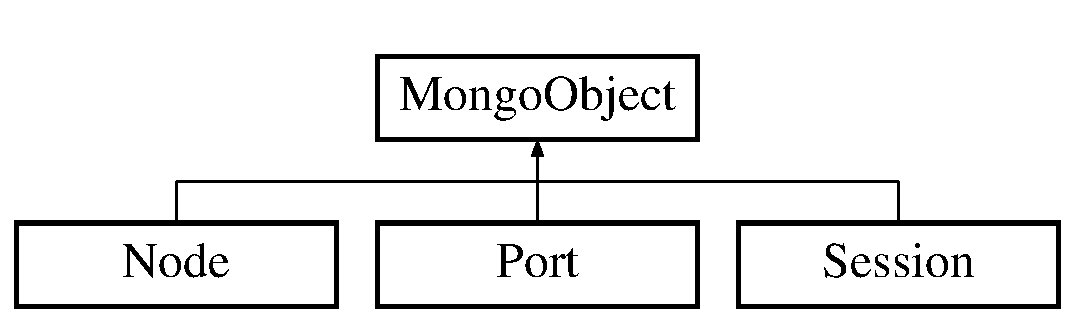
\includegraphics[height=2.000000cm]{class_mongo_object}
\end{center}
\end{figure}
\subsection*{Public Member Functions}
\begin{DoxyCompactItemize}
\item 
\hyperlink{class_mongo_object_ae0438efeae33db2bfeb3972e1196a8a9}{Mongo\+Object} ()
\item 
\hyperlink{class_mongo_object_a9e876f9d6e7cfcb7d4ce9046014e2b5f}{Mongo\+Object} (std\+::string name)
\item 
\hyperlink{class_mongo_object_ac1aba6b5189bca3feb08a698a01c1c30}{$\sim$\+Mongo\+Object} ()
\item 
bool \hyperlink{class_mongo_object_a7ef98cecb5c625a9c3e9a57373be41b8}{connect\+\_\+to\+\_\+db} (const std\+::string \&\hyperlink{class_mongo_object_a71e3fa5196ad3b496d0aa326d61e84e8}{uri\+\_\+string}, const std\+::string \&\hyperlink{class_mongo_object_a215dc4379af5ac81e19d245f5d5d37e0}{db\+\_\+string}, const std\+::string \&\hyperlink{class_mongo_object_ace5148b45dd674c73077a044d0233ed8}{app\+\_\+string}, const std\+::string \&\hyperlink{class_mongo_object_a59d2d926fd2f8048b1dab88b3e1fea5b}{collection\+\_\+string})
\item 
{\footnotesize template$<$typename T $>$ }\\bool \hyperlink{class_mongo_object_adbb80b6af3e780c81cc455f480507749}{connect\+\_\+object\+\_\+to\+\_\+db} (T o)
\item 
void \hyperlink{class_mongo_object_ae541414f753a8fd792cf0be163117b99}{disconnect\+\_\+from\+\_\+db} ()
\item 
bool \hyperlink{class_mongo_object_ae67113e87e4dadcd51c23aa373eba61d}{is\+\_\+connected\+\_\+to\+\_\+db} ()
\item 
virtual bool \hyperlink{class_mongo_object_a65971bad07dce8b649820f9dee5d0ae8}{write\+\_\+to\+\_\+db} ()
\item 
std\+::string \hyperlink{class_mongo_object_ad5165ed92020fba7d502a3556794ab4f}{create\+\_\+copy} ()
\item 
virtual bool \hyperlink{class_mongo_object_a729412e226c9964e13ba80688c3f5e00}{read\+\_\+from\+\_\+db} (const std\+::string \&oid\+\_\+string)
\item 
std\+::string \hyperlink{class_mongo_object_acde33629416d7f926737237264ac6ca1}{get\+\_\+json} ()
\item 
bool \hyperlink{class_mongo_object_adce8ffc4811a9d1c94701711f574bc34}{read\+\_\+json} (std\+::string json\+\_\+string)
\item 
std\+::string \hyperlink{class_mongo_object_ad155a8808f999f8e3dd0cfc055b33e2a}{get\+\_\+oid} ()
\item 
void \hyperlink{class_mongo_object_ac999ffe6b9b2ca261adff1eaf9da7e98}{set\+\_\+name} (std\+::string name)
\item 
virtual std\+::string \hyperlink{class_mongo_object_abd49d2dcea0ce5f49ebe9a8a9df97164}{get\+\_\+name} ()
\item 
{\footnotesize template$<$typename T $>$ }\\T \hyperlink{class_mongo_object_af0cf1568e5b1b87a971e93bba4ec0a40}{get\+\_\+singleton} (const char $\ast$key)
\item 
{\footnotesize template$<$typename T $>$ }\\void \hyperlink{class_mongo_object_a03a0d78b1f206aca81ff746edcd57c81}{set\+\_\+singleton} (const char $\ast$key, T value)
\item 
void \hyperlink{class_mongo_object_a9e80e38e5a4f40754ef48f2504e1613c}{set\+\_\+oid} (const char $\ast$key, bson\+\_\+oid\+\_\+t value)
\item 
{\footnotesize template$<$typename T $>$ }\\std\+::vector$<$ T $>$ \hyperlink{class_mongo_object_ae1002573afb58658162fb7f53cd0bffc}{get\+\_\+array} (const char $\ast$key)
\item 
{\footnotesize template$<$typename T $>$ }\\void \hyperlink{class_mongo_object_ac251f38eef739fb9e1418a20e7fcc7f7}{set\+\_\+array} (const char $\ast$key, std\+::vector$<$ T $>$ value)
\item 
std\+::string \hyperlink{class_mongo_object_a9f71ae755dac1db3e37cdee85329d163}{get\+\_\+json} (const char $\ast$key)
\item 
std\+::shared\+\_\+ptr$<$ \hyperlink{class_mongo_object}{Mongo\+Object} $>$ \hyperlink{class_mongo_object_a2136ceace181debba3d2c4fe07f947d8}{operator\mbox{[}$\,$\mbox{]}} (std\+::string key)
\item 
bool \hyperlink{class_mongo_object_a0050194f5bc8690e0db3b8217086e421}{operator==} (\hyperlink{class_mongo_object}{Mongo\+Object} const \&b)
\end{DoxyCompactItemize}
\subsection*{Protected Member Functions}
\begin{DoxyCompactItemize}
\item 
bson\+\_\+oid\+\_\+t \hyperlink{class_mongo_object_aaca278b427d042a63caf2962b5e76043}{get\+\_\+bson\+\_\+oid} ()
\item 
virtual bson\+\_\+t \hyperlink{class_mongo_object_ac21cbe104a818f7e6ee7dcfbb521e9e1}{get\+\_\+bson} ()
\item 
bson\+\_\+t \hyperlink{class_mongo_object_ac35c66d91e7297eb46313b98d01751cb}{get\+\_\+bson\+\_\+excluding} (const char $\ast$first,...)
\item 
const bson\+\_\+t $\ast$ \hyperlink{class_mongo_object_a196ea1b747a08f7ab525b8851ebc0b51}{get\+\_\+document} ()
\item 
const void \hyperlink{class_mongo_object_adb597533d8e167c3d6bafd28baef349c}{set\+\_\+document} (bson\+\_\+t b)
\item 
const void \hyperlink{class_mongo_object_ae51714acc607a67518862306fac509ee}{set\+\_\+document} (bson\+\_\+t $\ast$doc)
\item 
bool \hyperlink{class_mongo_object_ab43c880a2ae99890946e7edf3d232e5a}{write\+\_\+to\+\_\+db} (const bson\+\_\+t \&doc, int write\+\_\+option=0)
\begin{DoxyCompactList}\small\item\em Writes a B\+S\+ON document to the connected Mongo\+DB. \end{DoxyCompactList}\item 
bool \hyperlink{class_mongo_object_aecd244620f292e8368d1f593925eafbd}{read\+\_\+from\+\_\+db} ()
\item 
{\footnotesize template$<$typename T $>$ }\\void \hyperlink{class_mongo_object_ae8d85ac8089beca73773bd6189a2530c}{create\+\_\+oid\+\_\+dict\+\_\+in\+\_\+doc} (bson\+\_\+t $\ast$doc, std\+::string key, const std\+::map$<$ std\+::string, std\+::shared\+\_\+ptr$<$ T $>$$>$ \&mongo\+\_\+obj\+\_\+array)
\item 
{\footnotesize template$<$typename T $>$ }\\void \hyperlink{class_mongo_object_a56dccd703ae3e3e2193d57d31df12fd0}{append\+\_\+number\+\_\+array} (bson\+\_\+t $\ast$doc, std\+::string key, T \&values)
\item 
{\footnotesize template$<$typename T $>$ }\\void \hyperlink{class_mongo_object_a0b94ea01312b792e42b944399a4eb45c}{create\+\_\+oid\+\_\+array\+\_\+in\+\_\+doc} (bson\+\_\+t $\ast$doc, std\+::string target\+\_\+field\+\_\+name, const std\+::map$<$ std\+::string, std\+::shared\+\_\+ptr$<$ T $>$$>$ \&mongo\+\_\+obj\+\_\+array)
\item 
{\footnotesize template$<$typename T $>$ }\\bool \hyperlink{class_mongo_object_ab879c65bc54d59dc56cc0ca652756e10}{create\+\_\+and\+\_\+connect\+\_\+objects\+\_\+from\+\_\+oid\+\_\+doc} (const bson\+\_\+t $\ast$doc, const char $\ast$document\+\_\+name, std\+::map$<$ std\+::string, std\+::shared\+\_\+ptr$<$ T $>$$>$ $\ast$target\+\_\+map)
\item 
{\footnotesize template$<$typename T $>$ }\\bool \hyperlink{class_mongo_object_a830f8d398209664c866f2c437667cc5a}{create\+\_\+and\+\_\+connect\+\_\+objects\+\_\+from\+\_\+oid\+\_\+array} (const bson\+\_\+t $\ast$doc, const char $\ast$array\+\_\+name, std\+::map$<$ std\+::string, std\+::shared\+\_\+ptr$<$ T $>$$>$ $\ast$target\+\_\+map)
\end{DoxyCompactItemize}
\subsection*{Static Protected Member Functions}
\begin{DoxyCompactItemize}
\item 
static void \hyperlink{class_mongo_object_ab659c54f28b5e13c6cb2fc0fc8ad4635}{append\+\_\+string} (bson\+\_\+t $\ast$dst, std\+::string key, std\+::string content, size\+\_\+t size=0)
\item 
static const std\+::string \hyperlink{class_mongo_object_a33799f83d7343fc5385869f5a907aeea}{get\+\_\+string\+\_\+by\+\_\+key} (bson\+\_\+t $\ast$doc, std\+::string key)
\item 
static std\+::string \hyperlink{class_mongo_object_a9592c8baaed700c358dc26025e3bf166}{oid\+\_\+to\+\_\+string} (bson\+\_\+oid\+\_\+t oid)
\item 
static bool \hyperlink{class_mongo_object_ae9bff3fe8b82864f36e6cb7aa8f159b0}{string\+\_\+to\+\_\+oid} (const std\+::string \&oid\+\_\+string, bson\+\_\+oid\+\_\+t $\ast$oid)
\end{DoxyCompactItemize}
\subsection*{Protected Attributes}
\begin{DoxyCompactItemize}
\item 
std\+::string \hyperlink{class_mongo_object_a451655d98b9b515d856f7178b46e4b01}{object\+\_\+name}
\item 
bson\+\_\+t \hyperlink{class_mongo_object_aa143fbe117d6c12baf222be25555947b}{document}
\item 
std\+::string \hyperlink{class_mongo_object_a71e3fa5196ad3b496d0aa326d61e84e8}{uri\+\_\+string}
\item 
std\+::string \hyperlink{class_mongo_object_a215dc4379af5ac81e19d245f5d5d37e0}{db\+\_\+string}
\item 
std\+::string \hyperlink{class_mongo_object_ace5148b45dd674c73077a044d0233ed8}{app\+\_\+string}
\item 
std\+::string \hyperlink{class_mongo_object_a59d2d926fd2f8048b1dab88b3e1fea5b}{collection\+\_\+string}
\item 
bson\+\_\+oid\+\_\+t \hyperlink{class_mongo_object_a020a40224a752e6036d49ec22474d616}{oid\+\_\+document}
\item 
bson\+\_\+oid\+\_\+t \hyperlink{class_mongo_object_a4905c165b7b18f471ee56f8eb3f5e0f1}{oid\+\_\+precursor}
\item 
uint64\+\_\+t \hyperlink{class_mongo_object_a0ced4ff82fbee4e7213715994d690380}{time\+\_\+of\+\_\+death}
\end{DoxyCompactItemize}


\subsection{Detailed Description}
Connects the instance of database. 

Returns true if the instance of the to the DB.

Disconnects the the DB. 

\subsection{Constructor \& Destructor Documentation}
\mbox{\Hypertarget{class_mongo_object_ae0438efeae33db2bfeb3972e1196a8a9}\label{class_mongo_object_ae0438efeae33db2bfeb3972e1196a8a9}} 
\index{Mongo\+Object@{Mongo\+Object}!Mongo\+Object@{Mongo\+Object}}
\index{Mongo\+Object@{Mongo\+Object}!Mongo\+Object@{Mongo\+Object}}
\subsubsection{\texorpdfstring{Mongo\+Object()}{MongoObject()}\hspace{0.1cm}{\footnotesize\ttfamily [1/2]}}
{\footnotesize\ttfamily Mongo\+Object\+::\+Mongo\+Object (\begin{DoxyParamCaption}{ }\end{DoxyParamCaption})}

\mbox{\Hypertarget{class_mongo_object_a9e876f9d6e7cfcb7d4ce9046014e2b5f}\label{class_mongo_object_a9e876f9d6e7cfcb7d4ce9046014e2b5f}} 
\index{Mongo\+Object@{Mongo\+Object}!Mongo\+Object@{Mongo\+Object}}
\index{Mongo\+Object@{Mongo\+Object}!Mongo\+Object@{Mongo\+Object}}
\subsubsection{\texorpdfstring{Mongo\+Object()}{MongoObject()}\hspace{0.1cm}{\footnotesize\ttfamily [2/2]}}
{\footnotesize\ttfamily Mongo\+Object\+::\+Mongo\+Object (\begin{DoxyParamCaption}\item[{std\+::string}]{name }\end{DoxyParamCaption})}

\mbox{\Hypertarget{class_mongo_object_ac1aba6b5189bca3feb08a698a01c1c30}\label{class_mongo_object_ac1aba6b5189bca3feb08a698a01c1c30}} 
\index{Mongo\+Object@{Mongo\+Object}!````~Mongo\+Object@{$\sim$\+Mongo\+Object}}
\index{````~Mongo\+Object@{$\sim$\+Mongo\+Object}!Mongo\+Object@{Mongo\+Object}}
\subsubsection{\texorpdfstring{$\sim$\+Mongo\+Object()}{~MongoObject()}}
{\footnotesize\ttfamily Mongo\+Object\+::$\sim$\+Mongo\+Object (\begin{DoxyParamCaption}{ }\end{DoxyParamCaption})}



\subsection{Member Function Documentation}
\mbox{\Hypertarget{class_mongo_object_a56dccd703ae3e3e2193d57d31df12fd0}\label{class_mongo_object_a56dccd703ae3e3e2193d57d31df12fd0}} 
\index{Mongo\+Object@{Mongo\+Object}!append\+\_\+number\+\_\+array@{append\+\_\+number\+\_\+array}}
\index{append\+\_\+number\+\_\+array@{append\+\_\+number\+\_\+array}!Mongo\+Object@{Mongo\+Object}}
\subsubsection{\texorpdfstring{append\+\_\+number\+\_\+array()}{append\_number\_array()}}
{\footnotesize\ttfamily template$<$typename T $>$ \\
void Mongo\+Object\+::append\+\_\+number\+\_\+array (\begin{DoxyParamCaption}\item[{bson\+\_\+t $\ast$}]{doc,  }\item[{std\+::string}]{key,  }\item[{T \&}]{values }\end{DoxyParamCaption})\hspace{0.3cm}{\ttfamily [inline]}, {\ttfamily [protected]}}

\mbox{\Hypertarget{class_mongo_object_ab659c54f28b5e13c6cb2fc0fc8ad4635}\label{class_mongo_object_ab659c54f28b5e13c6cb2fc0fc8ad4635}} 
\index{Mongo\+Object@{Mongo\+Object}!append\+\_\+string@{append\+\_\+string}}
\index{append\+\_\+string@{append\+\_\+string}!Mongo\+Object@{Mongo\+Object}}
\subsubsection{\texorpdfstring{append\+\_\+string()}{append\_string()}}
{\footnotesize\ttfamily static void Mongo\+Object\+::append\+\_\+string (\begin{DoxyParamCaption}\item[{bson\+\_\+t $\ast$}]{dst,  }\item[{std\+::string}]{key,  }\item[{std\+::string}]{content,  }\item[{size\+\_\+t}]{size = {\ttfamily 0} }\end{DoxyParamCaption})\hspace{0.3cm}{\ttfamily [static]}, {\ttfamily [protected]}}

\mbox{\Hypertarget{class_mongo_object_adbb80b6af3e780c81cc455f480507749}\label{class_mongo_object_adbb80b6af3e780c81cc455f480507749}} 
\index{Mongo\+Object@{Mongo\+Object}!connect\+\_\+object\+\_\+to\+\_\+db@{connect\+\_\+object\+\_\+to\+\_\+db}}
\index{connect\+\_\+object\+\_\+to\+\_\+db@{connect\+\_\+object\+\_\+to\+\_\+db}!Mongo\+Object@{Mongo\+Object}}
\subsubsection{\texorpdfstring{connect\+\_\+object\+\_\+to\+\_\+db()}{connect\_object\_to\_db()}}
{\footnotesize\ttfamily template$<$typename T $>$ \\
bool Mongo\+Object\+::connect\+\_\+object\+\_\+to\+\_\+db (\begin{DoxyParamCaption}\item[{T}]{o }\end{DoxyParamCaption})\hspace{0.3cm}{\ttfamily [inline]}}

\mbox{\Hypertarget{class_mongo_object_a7ef98cecb5c625a9c3e9a57373be41b8}\label{class_mongo_object_a7ef98cecb5c625a9c3e9a57373be41b8}} 
\index{Mongo\+Object@{Mongo\+Object}!connect\+\_\+to\+\_\+db@{connect\+\_\+to\+\_\+db}}
\index{connect\+\_\+to\+\_\+db@{connect\+\_\+to\+\_\+db}!Mongo\+Object@{Mongo\+Object}}
\subsubsection{\texorpdfstring{connect\+\_\+to\+\_\+db()}{connect\_to\_db()}}
{\footnotesize\ttfamily bool Mongo\+Object\+::connect\+\_\+to\+\_\+db (\begin{DoxyParamCaption}\item[{const std\+::string \&}]{uri\+\_\+string,  }\item[{const std\+::string \&}]{db\+\_\+string,  }\item[{const std\+::string \&}]{app\+\_\+string,  }\item[{const std\+::string \&}]{collection\+\_\+string }\end{DoxyParamCaption})}


\begin{DoxyParams}{Parameters}
{\em uri\+\_\+string} & \\
\hline
{\em db\+\_\+string} & \\
\hline
{\em app\+\_\+string} & \\
\hline
{\em collection\+\_\+string} & \\
\hline
\end{DoxyParams}
\begin{DoxyReturn}{Returns}

\end{DoxyReturn}
\mbox{\Hypertarget{class_mongo_object_a830f8d398209664c866f2c437667cc5a}\label{class_mongo_object_a830f8d398209664c866f2c437667cc5a}} 
\index{Mongo\+Object@{Mongo\+Object}!create\+\_\+and\+\_\+connect\+\_\+objects\+\_\+from\+\_\+oid\+\_\+array@{create\+\_\+and\+\_\+connect\+\_\+objects\+\_\+from\+\_\+oid\+\_\+array}}
\index{create\+\_\+and\+\_\+connect\+\_\+objects\+\_\+from\+\_\+oid\+\_\+array@{create\+\_\+and\+\_\+connect\+\_\+objects\+\_\+from\+\_\+oid\+\_\+array}!Mongo\+Object@{Mongo\+Object}}
\subsubsection{\texorpdfstring{create\+\_\+and\+\_\+connect\+\_\+objects\+\_\+from\+\_\+oid\+\_\+array()}{create\_and\_connect\_objects\_from\_oid\_array()}}
{\footnotesize\ttfamily template$<$typename T $>$ \\
bool Mongo\+Object\+::create\+\_\+and\+\_\+connect\+\_\+objects\+\_\+from\+\_\+oid\+\_\+array (\begin{DoxyParamCaption}\item[{const bson\+\_\+t $\ast$}]{doc,  }\item[{const char $\ast$}]{array\+\_\+name,  }\item[{std\+::map$<$ std\+::string, std\+::shared\+\_\+ptr$<$ T $>$$>$ $\ast$}]{target\+\_\+map }\end{DoxyParamCaption})\hspace{0.3cm}{\ttfamily [inline]}, {\ttfamily [protected]}}

\mbox{\Hypertarget{class_mongo_object_ab879c65bc54d59dc56cc0ca652756e10}\label{class_mongo_object_ab879c65bc54d59dc56cc0ca652756e10}} 
\index{Mongo\+Object@{Mongo\+Object}!create\+\_\+and\+\_\+connect\+\_\+objects\+\_\+from\+\_\+oid\+\_\+doc@{create\+\_\+and\+\_\+connect\+\_\+objects\+\_\+from\+\_\+oid\+\_\+doc}}
\index{create\+\_\+and\+\_\+connect\+\_\+objects\+\_\+from\+\_\+oid\+\_\+doc@{create\+\_\+and\+\_\+connect\+\_\+objects\+\_\+from\+\_\+oid\+\_\+doc}!Mongo\+Object@{Mongo\+Object}}
\subsubsection{\texorpdfstring{create\+\_\+and\+\_\+connect\+\_\+objects\+\_\+from\+\_\+oid\+\_\+doc()}{create\_and\_connect\_objects\_from\_oid\_doc()}}
{\footnotesize\ttfamily template$<$typename T $>$ \\
bool Mongo\+Object\+::create\+\_\+and\+\_\+connect\+\_\+objects\+\_\+from\+\_\+oid\+\_\+doc (\begin{DoxyParamCaption}\item[{const bson\+\_\+t $\ast$}]{doc,  }\item[{const char $\ast$}]{document\+\_\+name,  }\item[{std\+::map$<$ std\+::string, std\+::shared\+\_\+ptr$<$ T $>$$>$ $\ast$}]{target\+\_\+map }\end{DoxyParamCaption})\hspace{0.3cm}{\ttfamily [inline]}, {\ttfamily [protected]}}

\mbox{\Hypertarget{class_mongo_object_ad5165ed92020fba7d502a3556794ab4f}\label{class_mongo_object_ad5165ed92020fba7d502a3556794ab4f}} 
\index{Mongo\+Object@{Mongo\+Object}!create\+\_\+copy@{create\+\_\+copy}}
\index{create\+\_\+copy@{create\+\_\+copy}!Mongo\+Object@{Mongo\+Object}}
\subsubsection{\texorpdfstring{create\+\_\+copy()}{create\_copy()}}
{\footnotesize\ttfamily std\+::string Mongo\+Object\+::create\+\_\+copy (\begin{DoxyParamCaption}{ }\end{DoxyParamCaption})}

\mbox{\Hypertarget{class_mongo_object_a0b94ea01312b792e42b944399a4eb45c}\label{class_mongo_object_a0b94ea01312b792e42b944399a4eb45c}} 
\index{Mongo\+Object@{Mongo\+Object}!create\+\_\+oid\+\_\+array\+\_\+in\+\_\+doc@{create\+\_\+oid\+\_\+array\+\_\+in\+\_\+doc}}
\index{create\+\_\+oid\+\_\+array\+\_\+in\+\_\+doc@{create\+\_\+oid\+\_\+array\+\_\+in\+\_\+doc}!Mongo\+Object@{Mongo\+Object}}
\subsubsection{\texorpdfstring{create\+\_\+oid\+\_\+array\+\_\+in\+\_\+doc()}{create\_oid\_array\_in\_doc()}}
{\footnotesize\ttfamily template$<$typename T $>$ \\
void Mongo\+Object\+::create\+\_\+oid\+\_\+array\+\_\+in\+\_\+doc (\begin{DoxyParamCaption}\item[{bson\+\_\+t $\ast$}]{doc,  }\item[{std\+::string}]{target\+\_\+field\+\_\+name,  }\item[{const std\+::map$<$ std\+::string, std\+::shared\+\_\+ptr$<$ T $>$$>$ \&}]{mongo\+\_\+obj\+\_\+array }\end{DoxyParamCaption})\hspace{0.3cm}{\ttfamily [inline]}, {\ttfamily [protected]}}

\mbox{\Hypertarget{class_mongo_object_ae8d85ac8089beca73773bd6189a2530c}\label{class_mongo_object_ae8d85ac8089beca73773bd6189a2530c}} 
\index{Mongo\+Object@{Mongo\+Object}!create\+\_\+oid\+\_\+dict\+\_\+in\+\_\+doc@{create\+\_\+oid\+\_\+dict\+\_\+in\+\_\+doc}}
\index{create\+\_\+oid\+\_\+dict\+\_\+in\+\_\+doc@{create\+\_\+oid\+\_\+dict\+\_\+in\+\_\+doc}!Mongo\+Object@{Mongo\+Object}}
\subsubsection{\texorpdfstring{create\+\_\+oid\+\_\+dict\+\_\+in\+\_\+doc()}{create\_oid\_dict\_in\_doc()}}
{\footnotesize\ttfamily template$<$typename T $>$ \\
void Mongo\+Object\+::create\+\_\+oid\+\_\+dict\+\_\+in\+\_\+doc (\begin{DoxyParamCaption}\item[{bson\+\_\+t $\ast$}]{doc,  }\item[{std\+::string}]{key,  }\item[{const std\+::map$<$ std\+::string, std\+::shared\+\_\+ptr$<$ T $>$$>$ \&}]{mongo\+\_\+obj\+\_\+array }\end{DoxyParamCaption})\hspace{0.3cm}{\ttfamily [inline]}, {\ttfamily [protected]}}

\mbox{\Hypertarget{class_mongo_object_ae541414f753a8fd792cf0be163117b99}\label{class_mongo_object_ae541414f753a8fd792cf0be163117b99}} 
\index{Mongo\+Object@{Mongo\+Object}!disconnect\+\_\+from\+\_\+db@{disconnect\+\_\+from\+\_\+db}}
\index{disconnect\+\_\+from\+\_\+db@{disconnect\+\_\+from\+\_\+db}!Mongo\+Object@{Mongo\+Object}}
\subsubsection{\texorpdfstring{disconnect\+\_\+from\+\_\+db()}{disconnect\_from\_db()}}
{\footnotesize\ttfamily void Mongo\+Object\+::disconnect\+\_\+from\+\_\+db (\begin{DoxyParamCaption}{ }\end{DoxyParamCaption})}

\mbox{\Hypertarget{class_mongo_object_ae1002573afb58658162fb7f53cd0bffc}\label{class_mongo_object_ae1002573afb58658162fb7f53cd0bffc}} 
\index{Mongo\+Object@{Mongo\+Object}!get\+\_\+array@{get\+\_\+array}}
\index{get\+\_\+array@{get\+\_\+array}!Mongo\+Object@{Mongo\+Object}}
\subsubsection{\texorpdfstring{get\+\_\+array()}{get\_array()}}
{\footnotesize\ttfamily template$<$typename T $>$ \\
std\+::vector$<$T$>$ Mongo\+Object\+::get\+\_\+array (\begin{DoxyParamCaption}\item[{const char $\ast$}]{key }\end{DoxyParamCaption})\hspace{0.3cm}{\ttfamily [inline]}}

\mbox{\Hypertarget{class_mongo_object_ac21cbe104a818f7e6ee7dcfbb521e9e1}\label{class_mongo_object_ac21cbe104a818f7e6ee7dcfbb521e9e1}} 
\index{Mongo\+Object@{Mongo\+Object}!get\+\_\+bson@{get\+\_\+bson}}
\index{get\+\_\+bson@{get\+\_\+bson}!Mongo\+Object@{Mongo\+Object}}
\subsubsection{\texorpdfstring{get\+\_\+bson()}{get\_bson()}}
{\footnotesize\ttfamily virtual bson\+\_\+t Mongo\+Object\+::get\+\_\+bson (\begin{DoxyParamCaption}{ }\end{DoxyParamCaption})\hspace{0.3cm}{\ttfamily [protected]}, {\ttfamily [virtual]}}



Reimplemented in \hyperlink{class_port_a746914b62d482cc81a901d254a03c560}{Port}, \hyperlink{class_node_a9568e1bba3436d78e77862902e328592}{Node}, and \hyperlink{class_session_aa517fe6138a0cc32e27ddf1eb7331520}{Session}.

\mbox{\Hypertarget{class_mongo_object_ac35c66d91e7297eb46313b98d01751cb}\label{class_mongo_object_ac35c66d91e7297eb46313b98d01751cb}} 
\index{Mongo\+Object@{Mongo\+Object}!get\+\_\+bson\+\_\+excluding@{get\+\_\+bson\+\_\+excluding}}
\index{get\+\_\+bson\+\_\+excluding@{get\+\_\+bson\+\_\+excluding}!Mongo\+Object@{Mongo\+Object}}
\subsubsection{\texorpdfstring{get\+\_\+bson\+\_\+excluding()}{get\_bson\_excluding()}}
{\footnotesize\ttfamily bson\+\_\+t Mongo\+Object\+::get\+\_\+bson\+\_\+excluding (\begin{DoxyParamCaption}\item[{const char $\ast$}]{first,  }\item[{}]{... }\end{DoxyParamCaption})\hspace{0.3cm}{\ttfamily [protected]}}

\mbox{\Hypertarget{class_mongo_object_aaca278b427d042a63caf2962b5e76043}\label{class_mongo_object_aaca278b427d042a63caf2962b5e76043}} 
\index{Mongo\+Object@{Mongo\+Object}!get\+\_\+bson\+\_\+oid@{get\+\_\+bson\+\_\+oid}}
\index{get\+\_\+bson\+\_\+oid@{get\+\_\+bson\+\_\+oid}!Mongo\+Object@{Mongo\+Object}}
\subsubsection{\texorpdfstring{get\+\_\+bson\+\_\+oid()}{get\_bson\_oid()}}
{\footnotesize\ttfamily bson\+\_\+oid\+\_\+t Mongo\+Object\+::get\+\_\+bson\+\_\+oid (\begin{DoxyParamCaption}{ }\end{DoxyParamCaption})\hspace{0.3cm}{\ttfamily [protected]}}

\mbox{\Hypertarget{class_mongo_object_a196ea1b747a08f7ab525b8851ebc0b51}\label{class_mongo_object_a196ea1b747a08f7ab525b8851ebc0b51}} 
\index{Mongo\+Object@{Mongo\+Object}!get\+\_\+document@{get\+\_\+document}}
\index{get\+\_\+document@{get\+\_\+document}!Mongo\+Object@{Mongo\+Object}}
\subsubsection{\texorpdfstring{get\+\_\+document()}{get\_document()}}
{\footnotesize\ttfamily const bson\+\_\+t$\ast$ Mongo\+Object\+::get\+\_\+document (\begin{DoxyParamCaption}{ }\end{DoxyParamCaption})\hspace{0.3cm}{\ttfamily [protected]}}

\mbox{\Hypertarget{class_mongo_object_acde33629416d7f926737237264ac6ca1}\label{class_mongo_object_acde33629416d7f926737237264ac6ca1}} 
\index{Mongo\+Object@{Mongo\+Object}!get\+\_\+json@{get\+\_\+json}}
\index{get\+\_\+json@{get\+\_\+json}!Mongo\+Object@{Mongo\+Object}}
\subsubsection{\texorpdfstring{get\+\_\+json()}{get\_json()}\hspace{0.1cm}{\footnotesize\ttfamily [1/2]}}
{\footnotesize\ttfamily std\+::string Mongo\+Object\+::get\+\_\+json (\begin{DoxyParamCaption}{ }\end{DoxyParamCaption})}

\mbox{\Hypertarget{class_mongo_object_a9f71ae755dac1db3e37cdee85329d163}\label{class_mongo_object_a9f71ae755dac1db3e37cdee85329d163}} 
\index{Mongo\+Object@{Mongo\+Object}!get\+\_\+json@{get\+\_\+json}}
\index{get\+\_\+json@{get\+\_\+json}!Mongo\+Object@{Mongo\+Object}}
\subsubsection{\texorpdfstring{get\+\_\+json()}{get\_json()}\hspace{0.1cm}{\footnotesize\ttfamily [2/2]}}
{\footnotesize\ttfamily std\+::string Mongo\+Object\+::get\+\_\+json (\begin{DoxyParamCaption}\item[{const char $\ast$}]{key }\end{DoxyParamCaption})\hspace{0.3cm}{\ttfamily [inline]}}

\mbox{\Hypertarget{class_mongo_object_abd49d2dcea0ce5f49ebe9a8a9df97164}\label{class_mongo_object_abd49d2dcea0ce5f49ebe9a8a9df97164}} 
\index{Mongo\+Object@{Mongo\+Object}!get\+\_\+name@{get\+\_\+name}}
\index{get\+\_\+name@{get\+\_\+name}!Mongo\+Object@{Mongo\+Object}}
\subsubsection{\texorpdfstring{get\+\_\+name()}{get\_name()}}
{\footnotesize\ttfamily virtual std\+::string Mongo\+Object\+::get\+\_\+name (\begin{DoxyParamCaption}{ }\end{DoxyParamCaption})\hspace{0.3cm}{\ttfamily [inline]}, {\ttfamily [virtual]}}



Reimplemented in \hyperlink{class_node_a0cc0386322fca056e49e49d869ade853}{Node}.

\mbox{\Hypertarget{class_mongo_object_ad155a8808f999f8e3dd0cfc055b33e2a}\label{class_mongo_object_ad155a8808f999f8e3dd0cfc055b33e2a}} 
\index{Mongo\+Object@{Mongo\+Object}!get\+\_\+oid@{get\+\_\+oid}}
\index{get\+\_\+oid@{get\+\_\+oid}!Mongo\+Object@{Mongo\+Object}}
\subsubsection{\texorpdfstring{get\+\_\+oid()}{get\_oid()}}
{\footnotesize\ttfamily std\+::string Mongo\+Object\+::get\+\_\+oid (\begin{DoxyParamCaption}{ }\end{DoxyParamCaption})}

\mbox{\Hypertarget{class_mongo_object_af0cf1568e5b1b87a971e93bba4ec0a40}\label{class_mongo_object_af0cf1568e5b1b87a971e93bba4ec0a40}} 
\index{Mongo\+Object@{Mongo\+Object}!get\+\_\+singleton@{get\+\_\+singleton}}
\index{get\+\_\+singleton@{get\+\_\+singleton}!Mongo\+Object@{Mongo\+Object}}
\subsubsection{\texorpdfstring{get\+\_\+singleton()}{get\_singleton()}}
{\footnotesize\ttfamily template$<$typename T $>$ \\
T Mongo\+Object\+::get\+\_\+singleton (\begin{DoxyParamCaption}\item[{const char $\ast$}]{key }\end{DoxyParamCaption})\hspace{0.3cm}{\ttfamily [inline]}}

\mbox{\Hypertarget{class_mongo_object_a33799f83d7343fc5385869f5a907aeea}\label{class_mongo_object_a33799f83d7343fc5385869f5a907aeea}} 
\index{Mongo\+Object@{Mongo\+Object}!get\+\_\+string\+\_\+by\+\_\+key@{get\+\_\+string\+\_\+by\+\_\+key}}
\index{get\+\_\+string\+\_\+by\+\_\+key@{get\+\_\+string\+\_\+by\+\_\+key}!Mongo\+Object@{Mongo\+Object}}
\subsubsection{\texorpdfstring{get\+\_\+string\+\_\+by\+\_\+key()}{get\_string\_by\_key()}}
{\footnotesize\ttfamily static const std\+::string Mongo\+Object\+::get\+\_\+string\+\_\+by\+\_\+key (\begin{DoxyParamCaption}\item[{bson\+\_\+t $\ast$}]{doc,  }\item[{std\+::string}]{key }\end{DoxyParamCaption})\hspace{0.3cm}{\ttfamily [static]}, {\ttfamily [protected]}}

\mbox{\Hypertarget{class_mongo_object_ae67113e87e4dadcd51c23aa373eba61d}\label{class_mongo_object_ae67113e87e4dadcd51c23aa373eba61d}} 
\index{Mongo\+Object@{Mongo\+Object}!is\+\_\+connected\+\_\+to\+\_\+db@{is\+\_\+connected\+\_\+to\+\_\+db}}
\index{is\+\_\+connected\+\_\+to\+\_\+db@{is\+\_\+connected\+\_\+to\+\_\+db}!Mongo\+Object@{Mongo\+Object}}
\subsubsection{\texorpdfstring{is\+\_\+connected\+\_\+to\+\_\+db()}{is\_connected\_to\_db()}}
{\footnotesize\ttfamily bool Mongo\+Object\+::is\+\_\+connected\+\_\+to\+\_\+db (\begin{DoxyParamCaption}{ }\end{DoxyParamCaption})}

\mbox{\Hypertarget{class_mongo_object_a9592c8baaed700c358dc26025e3bf166}\label{class_mongo_object_a9592c8baaed700c358dc26025e3bf166}} 
\index{Mongo\+Object@{Mongo\+Object}!oid\+\_\+to\+\_\+string@{oid\+\_\+to\+\_\+string}}
\index{oid\+\_\+to\+\_\+string@{oid\+\_\+to\+\_\+string}!Mongo\+Object@{Mongo\+Object}}
\subsubsection{\texorpdfstring{oid\+\_\+to\+\_\+string()}{oid\_to\_string()}}
{\footnotesize\ttfamily static std\+::string Mongo\+Object\+::oid\+\_\+to\+\_\+string (\begin{DoxyParamCaption}\item[{bson\+\_\+oid\+\_\+t}]{oid }\end{DoxyParamCaption})\hspace{0.3cm}{\ttfamily [inline]}, {\ttfamily [static]}, {\ttfamily [protected]}}

\mbox{\Hypertarget{class_mongo_object_a0050194f5bc8690e0db3b8217086e421}\label{class_mongo_object_a0050194f5bc8690e0db3b8217086e421}} 
\index{Mongo\+Object@{Mongo\+Object}!operator==@{operator==}}
\index{operator==@{operator==}!Mongo\+Object@{Mongo\+Object}}
\subsubsection{\texorpdfstring{operator==()}{operator==()}}
{\footnotesize\ttfamily bool Mongo\+Object\+::operator== (\begin{DoxyParamCaption}\item[{\hyperlink{class_mongo_object}{Mongo\+Object} const \&}]{b }\end{DoxyParamCaption})\hspace{0.3cm}{\ttfamily [inline]}}

\mbox{\Hypertarget{class_mongo_object_a2136ceace181debba3d2c4fe07f947d8}\label{class_mongo_object_a2136ceace181debba3d2c4fe07f947d8}} 
\index{Mongo\+Object@{Mongo\+Object}!operator\mbox{[}\mbox{]}@{operator[]}}
\index{operator\mbox{[}\mbox{]}@{operator[]}!Mongo\+Object@{Mongo\+Object}}
\subsubsection{\texorpdfstring{operator[]()}{operator[]()}}
{\footnotesize\ttfamily std\+::shared\+\_\+ptr$<$\hyperlink{class_mongo_object}{Mongo\+Object}$>$ Mongo\+Object\+::operator\mbox{[}$\,$\mbox{]} (\begin{DoxyParamCaption}\item[{std\+::string}]{key }\end{DoxyParamCaption})\hspace{0.3cm}{\ttfamily [inline]}}

\mbox{\Hypertarget{class_mongo_object_aecd244620f292e8368d1f593925eafbd}\label{class_mongo_object_aecd244620f292e8368d1f593925eafbd}} 
\index{Mongo\+Object@{Mongo\+Object}!read\+\_\+from\+\_\+db@{read\+\_\+from\+\_\+db}}
\index{read\+\_\+from\+\_\+db@{read\+\_\+from\+\_\+db}!Mongo\+Object@{Mongo\+Object}}
\subsubsection{\texorpdfstring{read\+\_\+from\+\_\+db()}{read\_from\_db()}\hspace{0.1cm}{\footnotesize\ttfamily [1/2]}}
{\footnotesize\ttfamily bool Mongo\+Object\+::read\+\_\+from\+\_\+db (\begin{DoxyParamCaption}{ }\end{DoxyParamCaption})\hspace{0.3cm}{\ttfamily [protected]}}

\mbox{\Hypertarget{class_mongo_object_a729412e226c9964e13ba80688c3f5e00}\label{class_mongo_object_a729412e226c9964e13ba80688c3f5e00}} 
\index{Mongo\+Object@{Mongo\+Object}!read\+\_\+from\+\_\+db@{read\+\_\+from\+\_\+db}}
\index{read\+\_\+from\+\_\+db@{read\+\_\+from\+\_\+db}!Mongo\+Object@{Mongo\+Object}}
\subsubsection{\texorpdfstring{read\+\_\+from\+\_\+db()}{read\_from\_db()}\hspace{0.1cm}{\footnotesize\ttfamily [2/2]}}
{\footnotesize\ttfamily virtual bool Mongo\+Object\+::read\+\_\+from\+\_\+db (\begin{DoxyParamCaption}\item[{const std\+::string \&}]{oid\+\_\+string }\end{DoxyParamCaption})\hspace{0.3cm}{\ttfamily [virtual]}}



Reimplemented in \hyperlink{class_port_a952b0b030c884147a36be7a04eb22183}{Port}, \hyperlink{class_session_a4f09644fd155a1d5640cedefe4aa42fc}{Session}, and \hyperlink{class_node_a60c605aced4420d3d6f6fe54b5a5b6bb}{Node}.

\mbox{\Hypertarget{class_mongo_object_adce8ffc4811a9d1c94701711f574bc34}\label{class_mongo_object_adce8ffc4811a9d1c94701711f574bc34}} 
\index{Mongo\+Object@{Mongo\+Object}!read\+\_\+json@{read\+\_\+json}}
\index{read\+\_\+json@{read\+\_\+json}!Mongo\+Object@{Mongo\+Object}}
\subsubsection{\texorpdfstring{read\+\_\+json()}{read\_json()}}
{\footnotesize\ttfamily bool Mongo\+Object\+::read\+\_\+json (\begin{DoxyParamCaption}\item[{std\+::string}]{json\+\_\+string }\end{DoxyParamCaption})}

\mbox{\Hypertarget{class_mongo_object_ac251f38eef739fb9e1418a20e7fcc7f7}\label{class_mongo_object_ac251f38eef739fb9e1418a20e7fcc7f7}} 
\index{Mongo\+Object@{Mongo\+Object}!set\+\_\+array@{set\+\_\+array}}
\index{set\+\_\+array@{set\+\_\+array}!Mongo\+Object@{Mongo\+Object}}
\subsubsection{\texorpdfstring{set\+\_\+array()}{set\_array()}}
{\footnotesize\ttfamily template$<$typename T $>$ \\
void Mongo\+Object\+::set\+\_\+array (\begin{DoxyParamCaption}\item[{const char $\ast$}]{key,  }\item[{std\+::vector$<$ T $>$}]{value }\end{DoxyParamCaption})\hspace{0.3cm}{\ttfamily [inline]}}

\mbox{\Hypertarget{class_mongo_object_adb597533d8e167c3d6bafd28baef349c}\label{class_mongo_object_adb597533d8e167c3d6bafd28baef349c}} 
\index{Mongo\+Object@{Mongo\+Object}!set\+\_\+document@{set\+\_\+document}}
\index{set\+\_\+document@{set\+\_\+document}!Mongo\+Object@{Mongo\+Object}}
\subsubsection{\texorpdfstring{set\+\_\+document()}{set\_document()}\hspace{0.1cm}{\footnotesize\ttfamily [1/2]}}
{\footnotesize\ttfamily const void Mongo\+Object\+::set\+\_\+document (\begin{DoxyParamCaption}\item[{bson\+\_\+t}]{b }\end{DoxyParamCaption})\hspace{0.3cm}{\ttfamily [inline]}, {\ttfamily [protected]}}

\mbox{\Hypertarget{class_mongo_object_ae51714acc607a67518862306fac509ee}\label{class_mongo_object_ae51714acc607a67518862306fac509ee}} 
\index{Mongo\+Object@{Mongo\+Object}!set\+\_\+document@{set\+\_\+document}}
\index{set\+\_\+document@{set\+\_\+document}!Mongo\+Object@{Mongo\+Object}}
\subsubsection{\texorpdfstring{set\+\_\+document()}{set\_document()}\hspace{0.1cm}{\footnotesize\ttfamily [2/2]}}
{\footnotesize\ttfamily const void Mongo\+Object\+::set\+\_\+document (\begin{DoxyParamCaption}\item[{bson\+\_\+t $\ast$}]{doc }\end{DoxyParamCaption})\hspace{0.3cm}{\ttfamily [inline]}, {\ttfamily [protected]}}

\mbox{\Hypertarget{class_mongo_object_ac999ffe6b9b2ca261adff1eaf9da7e98}\label{class_mongo_object_ac999ffe6b9b2ca261adff1eaf9da7e98}} 
\index{Mongo\+Object@{Mongo\+Object}!set\+\_\+name@{set\+\_\+name}}
\index{set\+\_\+name@{set\+\_\+name}!Mongo\+Object@{Mongo\+Object}}
\subsubsection{\texorpdfstring{set\+\_\+name()}{set\_name()}}
{\footnotesize\ttfamily void Mongo\+Object\+::set\+\_\+name (\begin{DoxyParamCaption}\item[{std\+::string}]{name }\end{DoxyParamCaption})\hspace{0.3cm}{\ttfamily [inline]}}

\mbox{\Hypertarget{class_mongo_object_a9e80e38e5a4f40754ef48f2504e1613c}\label{class_mongo_object_a9e80e38e5a4f40754ef48f2504e1613c}} 
\index{Mongo\+Object@{Mongo\+Object}!set\+\_\+oid@{set\+\_\+oid}}
\index{set\+\_\+oid@{set\+\_\+oid}!Mongo\+Object@{Mongo\+Object}}
\subsubsection{\texorpdfstring{set\+\_\+oid()}{set\_oid()}}
{\footnotesize\ttfamily void Mongo\+Object\+::set\+\_\+oid (\begin{DoxyParamCaption}\item[{const char $\ast$}]{key,  }\item[{bson\+\_\+oid\+\_\+t}]{value }\end{DoxyParamCaption})}

\mbox{\Hypertarget{class_mongo_object_a03a0d78b1f206aca81ff746edcd57c81}\label{class_mongo_object_a03a0d78b1f206aca81ff746edcd57c81}} 
\index{Mongo\+Object@{Mongo\+Object}!set\+\_\+singleton@{set\+\_\+singleton}}
\index{set\+\_\+singleton@{set\+\_\+singleton}!Mongo\+Object@{Mongo\+Object}}
\subsubsection{\texorpdfstring{set\+\_\+singleton()}{set\_singleton()}}
{\footnotesize\ttfamily template$<$typename T $>$ \\
void Mongo\+Object\+::set\+\_\+singleton (\begin{DoxyParamCaption}\item[{const char $\ast$}]{key,  }\item[{T}]{value }\end{DoxyParamCaption})\hspace{0.3cm}{\ttfamily [inline]}}

\mbox{\Hypertarget{class_mongo_object_ae9bff3fe8b82864f36e6cb7aa8f159b0}\label{class_mongo_object_ae9bff3fe8b82864f36e6cb7aa8f159b0}} 
\index{Mongo\+Object@{Mongo\+Object}!string\+\_\+to\+\_\+oid@{string\+\_\+to\+\_\+oid}}
\index{string\+\_\+to\+\_\+oid@{string\+\_\+to\+\_\+oid}!Mongo\+Object@{Mongo\+Object}}
\subsubsection{\texorpdfstring{string\+\_\+to\+\_\+oid()}{string\_to\_oid()}}
{\footnotesize\ttfamily static bool Mongo\+Object\+::string\+\_\+to\+\_\+oid (\begin{DoxyParamCaption}\item[{const std\+::string \&}]{oid\+\_\+string,  }\item[{bson\+\_\+oid\+\_\+t $\ast$}]{oid }\end{DoxyParamCaption})\hspace{0.3cm}{\ttfamily [static]}, {\ttfamily [protected]}}

\mbox{\Hypertarget{class_mongo_object_ab43c880a2ae99890946e7edf3d232e5a}\label{class_mongo_object_ab43c880a2ae99890946e7edf3d232e5a}} 
\index{Mongo\+Object@{Mongo\+Object}!write\+\_\+to\+\_\+db@{write\+\_\+to\+\_\+db}}
\index{write\+\_\+to\+\_\+db@{write\+\_\+to\+\_\+db}!Mongo\+Object@{Mongo\+Object}}
\subsubsection{\texorpdfstring{write\+\_\+to\+\_\+db()}{write\_to\_db()}\hspace{0.1cm}{\footnotesize\ttfamily [1/2]}}
{\footnotesize\ttfamily bool Mongo\+Object\+::write\+\_\+to\+\_\+db (\begin{DoxyParamCaption}\item[{const bson\+\_\+t \&}]{doc,  }\item[{int}]{write\+\_\+option = {\ttfamily 0} }\end{DoxyParamCaption})\hspace{0.3cm}{\ttfamily [protected]}}



Writes a B\+S\+ON document to the connected Mongo\+DB. 


\begin{DoxyParams}{Parameters}
{\em doc} & a pointer to the B\+S\+ON document that is written to the Mongo\+DB \\
\hline
{\em write\+\_\+option} & integer specifying the write mode -\/ 1\+: replaces the document (no upsert), 2\+: insert the document das a new document, default\+: updates an existing document.\\
\hline
\end{DoxyParams}
\begin{DoxyReturn}{Returns}
true in case of a successful write. 
\end{DoxyReturn}
\mbox{\Hypertarget{class_mongo_object_a65971bad07dce8b649820f9dee5d0ae8}\label{class_mongo_object_a65971bad07dce8b649820f9dee5d0ae8}} 
\index{Mongo\+Object@{Mongo\+Object}!write\+\_\+to\+\_\+db@{write\+\_\+to\+\_\+db}}
\index{write\+\_\+to\+\_\+db@{write\+\_\+to\+\_\+db}!Mongo\+Object@{Mongo\+Object}}
\subsubsection{\texorpdfstring{write\+\_\+to\+\_\+db()}{write\_to\_db()}\hspace{0.1cm}{\footnotesize\ttfamily [2/2]}}
{\footnotesize\ttfamily virtual bool Mongo\+Object\+::write\+\_\+to\+\_\+db (\begin{DoxyParamCaption}{ }\end{DoxyParamCaption})\hspace{0.3cm}{\ttfamily [virtual]}}



Reimplemented in \hyperlink{class_port_a052c0ba97e0a53e45d973d4bc31fa615}{Port}, \hyperlink{class_node_ad5cacb320e423275faef1bfc8c7a365b}{Node}, and \hyperlink{class_session_a513e5436b4c990985300246bb39d9f5c}{Session}.



\subsection{Member Data Documentation}
\mbox{\Hypertarget{class_mongo_object_ace5148b45dd674c73077a044d0233ed8}\label{class_mongo_object_ace5148b45dd674c73077a044d0233ed8}} 
\index{Mongo\+Object@{Mongo\+Object}!app\+\_\+string@{app\+\_\+string}}
\index{app\+\_\+string@{app\+\_\+string}!Mongo\+Object@{Mongo\+Object}}
\subsubsection{\texorpdfstring{app\+\_\+string}{app\_string}}
{\footnotesize\ttfamily std\+::string Mongo\+Object\+::app\+\_\+string\hspace{0.3cm}{\ttfamily [protected]}}

\mbox{\Hypertarget{class_mongo_object_a59d2d926fd2f8048b1dab88b3e1fea5b}\label{class_mongo_object_a59d2d926fd2f8048b1dab88b3e1fea5b}} 
\index{Mongo\+Object@{Mongo\+Object}!collection\+\_\+string@{collection\+\_\+string}}
\index{collection\+\_\+string@{collection\+\_\+string}!Mongo\+Object@{Mongo\+Object}}
\subsubsection{\texorpdfstring{collection\+\_\+string}{collection\_string}}
{\footnotesize\ttfamily std\+::string Mongo\+Object\+::collection\+\_\+string\hspace{0.3cm}{\ttfamily [protected]}}

\mbox{\Hypertarget{class_mongo_object_a215dc4379af5ac81e19d245f5d5d37e0}\label{class_mongo_object_a215dc4379af5ac81e19d245f5d5d37e0}} 
\index{Mongo\+Object@{Mongo\+Object}!db\+\_\+string@{db\+\_\+string}}
\index{db\+\_\+string@{db\+\_\+string}!Mongo\+Object@{Mongo\+Object}}
\subsubsection{\texorpdfstring{db\+\_\+string}{db\_string}}
{\footnotesize\ttfamily std\+::string Mongo\+Object\+::db\+\_\+string\hspace{0.3cm}{\ttfamily [protected]}}

\mbox{\Hypertarget{class_mongo_object_aa143fbe117d6c12baf222be25555947b}\label{class_mongo_object_aa143fbe117d6c12baf222be25555947b}} 
\index{Mongo\+Object@{Mongo\+Object}!document@{document}}
\index{document@{document}!Mongo\+Object@{Mongo\+Object}}
\subsubsection{\texorpdfstring{document}{document}}
{\footnotesize\ttfamily bson\+\_\+t Mongo\+Object\+::document\hspace{0.3cm}{\ttfamily [protected]}}

\mbox{\Hypertarget{class_mongo_object_a451655d98b9b515d856f7178b46e4b01}\label{class_mongo_object_a451655d98b9b515d856f7178b46e4b01}} 
\index{Mongo\+Object@{Mongo\+Object}!object\+\_\+name@{object\+\_\+name}}
\index{object\+\_\+name@{object\+\_\+name}!Mongo\+Object@{Mongo\+Object}}
\subsubsection{\texorpdfstring{object\+\_\+name}{object\_name}}
{\footnotesize\ttfamily std\+::string Mongo\+Object\+::object\+\_\+name\hspace{0.3cm}{\ttfamily [protected]}}

\mbox{\Hypertarget{class_mongo_object_a020a40224a752e6036d49ec22474d616}\label{class_mongo_object_a020a40224a752e6036d49ec22474d616}} 
\index{Mongo\+Object@{Mongo\+Object}!oid\+\_\+document@{oid\+\_\+document}}
\index{oid\+\_\+document@{oid\+\_\+document}!Mongo\+Object@{Mongo\+Object}}
\subsubsection{\texorpdfstring{oid\+\_\+document}{oid\_document}}
{\footnotesize\ttfamily bson\+\_\+oid\+\_\+t Mongo\+Object\+::oid\+\_\+document\hspace{0.3cm}{\ttfamily [protected]}}

\mbox{\Hypertarget{class_mongo_object_a4905c165b7b18f471ee56f8eb3f5e0f1}\label{class_mongo_object_a4905c165b7b18f471ee56f8eb3f5e0f1}} 
\index{Mongo\+Object@{Mongo\+Object}!oid\+\_\+precursor@{oid\+\_\+precursor}}
\index{oid\+\_\+precursor@{oid\+\_\+precursor}!Mongo\+Object@{Mongo\+Object}}
\subsubsection{\texorpdfstring{oid\+\_\+precursor}{oid\_precursor}}
{\footnotesize\ttfamily bson\+\_\+oid\+\_\+t Mongo\+Object\+::oid\+\_\+precursor\hspace{0.3cm}{\ttfamily [protected]}}

\mbox{\Hypertarget{class_mongo_object_a0ced4ff82fbee4e7213715994d690380}\label{class_mongo_object_a0ced4ff82fbee4e7213715994d690380}} 
\index{Mongo\+Object@{Mongo\+Object}!time\+\_\+of\+\_\+death@{time\+\_\+of\+\_\+death}}
\index{time\+\_\+of\+\_\+death@{time\+\_\+of\+\_\+death}!Mongo\+Object@{Mongo\+Object}}
\subsubsection{\texorpdfstring{time\+\_\+of\+\_\+death}{time\_of\_death}}
{\footnotesize\ttfamily uint64\+\_\+t Mongo\+Object\+::time\+\_\+of\+\_\+death\hspace{0.3cm}{\ttfamily [protected]}}

\mbox{\Hypertarget{class_mongo_object_a71e3fa5196ad3b496d0aa326d61e84e8}\label{class_mongo_object_a71e3fa5196ad3b496d0aa326d61e84e8}} 
\index{Mongo\+Object@{Mongo\+Object}!uri\+\_\+string@{uri\+\_\+string}}
\index{uri\+\_\+string@{uri\+\_\+string}!Mongo\+Object@{Mongo\+Object}}
\subsubsection{\texorpdfstring{uri\+\_\+string}{uri\_string}}
{\footnotesize\ttfamily std\+::string Mongo\+Object\+::uri\+\_\+string\hspace{0.3cm}{\ttfamily [protected]}}



The documentation for this class was generated from the following file\+:\begin{DoxyCompactItemize}
\item 
include/\hyperlink{_mongo_object_8h}{Mongo\+Object.\+h}\end{DoxyCompactItemize}

\hypertarget{class_node}{}\section{Node Class Reference}
\label{class_node}\index{Node@{Node}}


{\ttfamily \#include $<$Node.\+h$>$}

Inheritance diagram for Node\+:\begin{figure}[H]
\begin{center}
\leavevmode
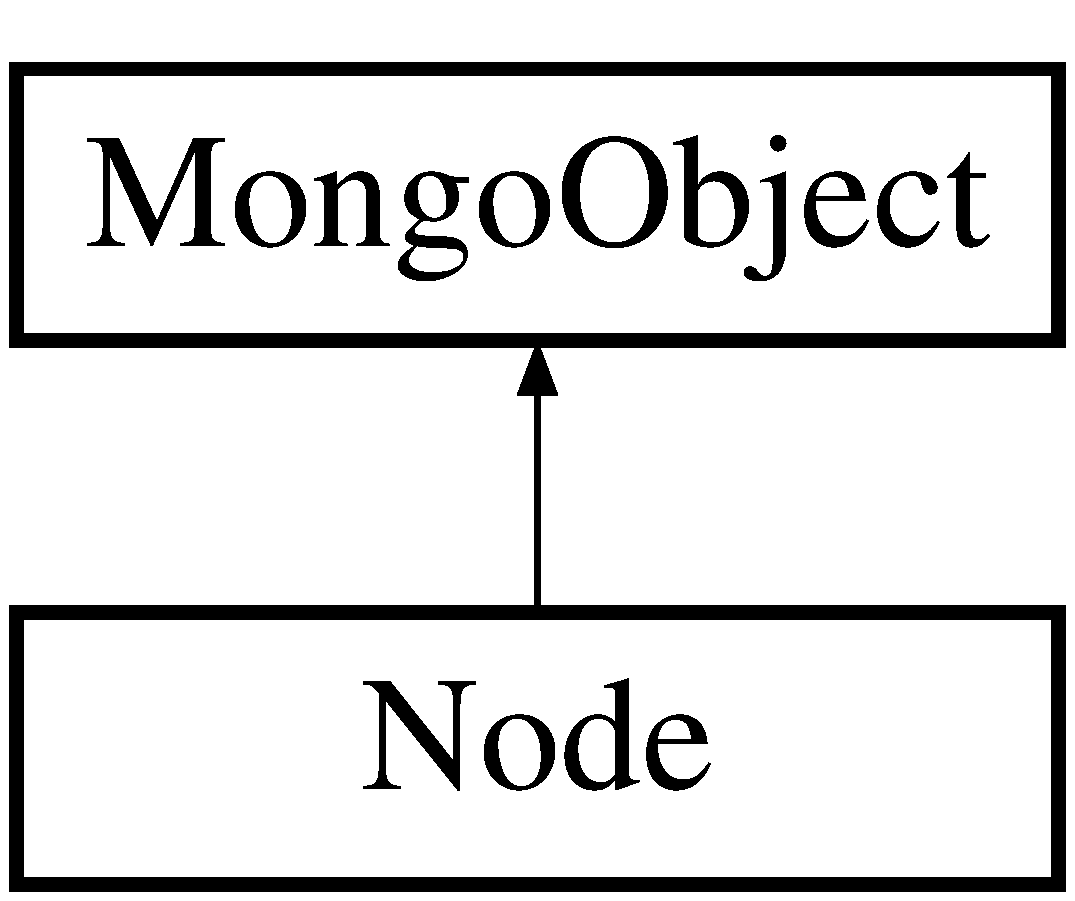
\includegraphics[height=2.000000cm]{class_node}
\end{center}
\end{figure}
\subsection*{Public Member Functions}
\begin{DoxyCompactItemize}
\item 
\hyperlink{class_node_ad7a34779cad45d997bfd6d3d8043c75f}{Node} ()
\item 
\hyperlink{class_node_afceb8877cfab44e0eda5ae3a88513242}{Node} (std\+::string name)
\item 
\hyperlink{class_node_acdcee054c893b696b5bc08a8eba1a668}{Node} (std\+::map$<$ std\+::string, std\+::shared\+\_\+ptr$<$ \hyperlink{class_port}{Port} $>$$>$ ports)
\item 
\hyperlink{class_node_aa0840c3cb5c7159be6d992adecd2097c}{$\sim$\+Node} ()
\item 
bool \hyperlink{class_node_a60c605aced4420d3d6f6fe54b5a5b6bb}{read\+\_\+from\+\_\+db} (const std\+::string \&oid\+\_\+string) final
\item 
void \hyperlink{class_node_a0a3c8430a9e5b6b725c87bbcf7adc54b}{evaluate} ()
\item 
bool \hyperlink{class_node_a8d821a6df3cd9504fefc551d5bd0a64f}{is\+\_\+valid} ()
\item 
bool \hyperlink{class_node_adb04f5aa8b454b19db663b3f240e9061}{inputs\+\_\+valid} ()
\item 
bool \hyperlink{class_node_ad5cacb320e423275faef1bfc8c7a365b}{write\+\_\+to\+\_\+db} () final
\item 
bson\+\_\+t \hyperlink{class_node_a9568e1bba3436d78e77862902e328592}{get\+\_\+bson} ()
\item 
std\+::string \hyperlink{class_node_a0cc0386322fca056e49e49d869ade853}{get\+\_\+name} ()
\item 
std\+::map$<$ std\+::string, std\+::shared\+\_\+ptr$<$ \hyperlink{class_port}{Port} $>$ $>$ \hyperlink{class_node_aab2f990047525bd3bfe7be041a8a201c}{get\+\_\+input\+\_\+ports} ()
\item 
std\+::map$<$ std\+::string, std\+::shared\+\_\+ptr$<$ \hyperlink{class_port}{Port} $>$ $>$ \hyperlink{class_node_a060160b85a15190fcf98fa0a3f9ec4e6}{get\+\_\+output\+\_\+ports} ()
\item 
std\+::map$<$ std\+::string, std\+::shared\+\_\+ptr$<$ \hyperlink{class_port}{Port} $>$ $>$ \hyperlink{class_node_a90fc0096ba3a5094f0696dde1dd5b08d}{get\+\_\+ports} ()
\item 
std\+::shared\+\_\+ptr$<$ \hyperlink{class_port}{Port} $>$ \hyperlink{class_node_a71b857799058e56ccb9593a69fc675bc}{get\+\_\+port} (const std\+::string \&port\+\_\+name)
\item 
void \hyperlink{class_node_a139ab3c04753749cc35d2ff8c268c248}{add\+\_\+port} (std\+::string key, std\+::shared\+\_\+ptr$<$ \hyperlink{class_port}{Port} $>$, bool is\+\_\+source, bool fill\+\_\+in\+\_\+out=true)
\item 
void \hyperlink{class_node_ac0b67acb7c270cf38579356325ee6e9c}{add\+\_\+input\+\_\+port} (std\+::string key, std\+::shared\+\_\+ptr$<$ \hyperlink{class_port}{Port} $>$)
\item 
void \hyperlink{class_node_a9df0ba6b43f1b59fd0bce26470b906ba}{add\+\_\+output\+\_\+port} (std\+::string key, std\+::shared\+\_\+ptr$<$ \hyperlink{class_port}{Port} $>$)
\item 
std\+::shared\+\_\+ptr$<$ \hyperlink{class_port}{Port} $>$ \hyperlink{class_node_a89e7f8e74b09395e5a2362bcef664ee9}{get\+\_\+input\+\_\+port} (const std\+::string \&port\+\_\+name)
\item 
std\+::shared\+\_\+ptr$<$ \hyperlink{class_port}{Port} $>$ \hyperlink{class_node_a98f6937be16c29da2ea37b0ad51cb463}{get\+\_\+output\+\_\+port} (const std\+::string \&port\+\_\+name)
\item 
void \hyperlink{class_node_a924146fb76ec67a78971f91e93418527}{set\+\_\+callback} (std\+::shared\+\_\+ptr$<$ \hyperlink{class_node_callback}{Node\+Callback} $>$ cb)
\item 
void \hyperlink{class_node_afda492d07d8c3ed0e714d0249e015ffa}{set\+\_\+callback} (std\+::string \hyperlink{class_node_a3755609fd44cf5b86c8a7d1f94d9747b}{callback}, std\+::string \hyperlink{class_node_a290c95a63ae639d150355764ea1f4b54}{callback\+\_\+type})
\item 
void \hyperlink{class_node_ab9fe9ebcddc19a16dc518fd29e584da8}{set\+\_\+node\+\_\+to\+\_\+invalid} ()
\end{DoxyCompactItemize}
\subsection*{Public Attributes}
\begin{DoxyCompactItemize}
\item 
std\+::shared\+\_\+ptr$<$ \hyperlink{class_node_callback}{Node\+Callback} $>$ \hyperlink{class_node_a9bc5e92a6565a4addbbcadea93889e85}{callback\+\_\+class}
\end{DoxyCompactItemize}
\subsection*{Protected Member Functions}
\begin{DoxyCompactItemize}
\item 
void \hyperlink{class_node_a4ef31790680213bff2306ec34941941c}{fill\+\_\+input\+\_\+output\+\_\+port\+\_\+lookups} ()
\end{DoxyCompactItemize}
\subsection*{Protected Attributes}
\begin{DoxyCompactItemize}
\item 
rttr\+::method \hyperlink{class_node_a34e4ef7089672adaa8aa31277aa5f159}{meth\+\_\+} = rttr\+::type\+::get\+\_\+global\+\_\+method(\char`\"{}nothing\char`\"{})
\item 
std\+::map$<$ std\+::string, std\+::shared\+\_\+ptr$<$ \hyperlink{class_port}{Port} $>$ $>$ \hyperlink{class_node_a2970ced9f376dd6c5d512d0bbb7cbb54}{in\+\_\+}
\item 
std\+::map$<$ std\+::string, std\+::shared\+\_\+ptr$<$ \hyperlink{class_port}{Port} $>$ $>$ \hyperlink{class_node_a324497db3924989e08e8ee0411d5972e}{out\+\_\+}
\item 
std\+::string \hyperlink{class_node_a3755609fd44cf5b86c8a7d1f94d9747b}{callback}
\item 
std\+::string \hyperlink{class_node_aa6465260fcaaecbb7bc8847dbbeb3ba6}{callback\+\_\+type\+\_\+string}
\item 
int \hyperlink{class_node_a290c95a63ae639d150355764ea1f4b54}{callback\+\_\+type}
\end{DoxyCompactItemize}
\subsection*{Additional Inherited Members}


\subsection{Constructor \& Destructor Documentation}
\mbox{\Hypertarget{class_node_ad7a34779cad45d997bfd6d3d8043c75f}\label{class_node_ad7a34779cad45d997bfd6d3d8043c75f}} 
\index{Node@{Node}!Node@{Node}}
\index{Node@{Node}!Node@{Node}}
\subsubsection{\texorpdfstring{Node()}{Node()}\hspace{0.1cm}{\footnotesize\ttfamily [1/3]}}
{\footnotesize\ttfamily Node\+::\+Node (\begin{DoxyParamCaption}{ }\end{DoxyParamCaption})}

\mbox{\Hypertarget{class_node_afceb8877cfab44e0eda5ae3a88513242}\label{class_node_afceb8877cfab44e0eda5ae3a88513242}} 
\index{Node@{Node}!Node@{Node}}
\index{Node@{Node}!Node@{Node}}
\subsubsection{\texorpdfstring{Node()}{Node()}\hspace{0.1cm}{\footnotesize\ttfamily [2/3]}}
{\footnotesize\ttfamily Node\+::\+Node (\begin{DoxyParamCaption}\item[{std\+::string}]{name }\end{DoxyParamCaption})}

\mbox{\Hypertarget{class_node_acdcee054c893b696b5bc08a8eba1a668}\label{class_node_acdcee054c893b696b5bc08a8eba1a668}} 
\index{Node@{Node}!Node@{Node}}
\index{Node@{Node}!Node@{Node}}
\subsubsection{\texorpdfstring{Node()}{Node()}\hspace{0.1cm}{\footnotesize\ttfamily [3/3]}}
{\footnotesize\ttfamily Node\+::\+Node (\begin{DoxyParamCaption}\item[{std\+::map$<$ std\+::string, std\+::shared\+\_\+ptr$<$ \hyperlink{class_port}{Port} $>$$>$}]{ports }\end{DoxyParamCaption})}

\mbox{\Hypertarget{class_node_aa0840c3cb5c7159be6d992adecd2097c}\label{class_node_aa0840c3cb5c7159be6d992adecd2097c}} 
\index{Node@{Node}!````~Node@{$\sim$\+Node}}
\index{````~Node@{$\sim$\+Node}!Node@{Node}}
\subsubsection{\texorpdfstring{$\sim$\+Node()}{~Node()}}
{\footnotesize\ttfamily Node\+::$\sim$\+Node (\begin{DoxyParamCaption}{ }\end{DoxyParamCaption})}



\subsection{Member Function Documentation}
\mbox{\Hypertarget{class_node_ac0b67acb7c270cf38579356325ee6e9c}\label{class_node_ac0b67acb7c270cf38579356325ee6e9c}} 
\index{Node@{Node}!add\+\_\+input\+\_\+port@{add\+\_\+input\+\_\+port}}
\index{add\+\_\+input\+\_\+port@{add\+\_\+input\+\_\+port}!Node@{Node}}
\subsubsection{\texorpdfstring{add\+\_\+input\+\_\+port()}{add\_input\_port()}}
{\footnotesize\ttfamily void Node\+::add\+\_\+input\+\_\+port (\begin{DoxyParamCaption}\item[{std\+::string}]{key,  }\item[{std\+::shared\+\_\+ptr$<$ \hyperlink{class_port}{Port} $>$}]{ }\end{DoxyParamCaption})}

\mbox{\Hypertarget{class_node_a9df0ba6b43f1b59fd0bce26470b906ba}\label{class_node_a9df0ba6b43f1b59fd0bce26470b906ba}} 
\index{Node@{Node}!add\+\_\+output\+\_\+port@{add\+\_\+output\+\_\+port}}
\index{add\+\_\+output\+\_\+port@{add\+\_\+output\+\_\+port}!Node@{Node}}
\subsubsection{\texorpdfstring{add\+\_\+output\+\_\+port()}{add\_output\_port()}}
{\footnotesize\ttfamily void Node\+::add\+\_\+output\+\_\+port (\begin{DoxyParamCaption}\item[{std\+::string}]{key,  }\item[{std\+::shared\+\_\+ptr$<$ \hyperlink{class_port}{Port} $>$}]{ }\end{DoxyParamCaption})}

\mbox{\Hypertarget{class_node_a139ab3c04753749cc35d2ff8c268c248}\label{class_node_a139ab3c04753749cc35d2ff8c268c248}} 
\index{Node@{Node}!add\+\_\+port@{add\+\_\+port}}
\index{add\+\_\+port@{add\+\_\+port}!Node@{Node}}
\subsubsection{\texorpdfstring{add\+\_\+port()}{add\_port()}}
{\footnotesize\ttfamily void Node\+::add\+\_\+port (\begin{DoxyParamCaption}\item[{std\+::string}]{key,  }\item[{std\+::shared\+\_\+ptr$<$ \hyperlink{class_port}{Port} $>$}]{,  }\item[{bool}]{is\+\_\+source,  }\item[{bool}]{fill\+\_\+in\+\_\+out = {\ttfamily true} }\end{DoxyParamCaption})}

\mbox{\Hypertarget{class_node_a0a3c8430a9e5b6b725c87bbcf7adc54b}\label{class_node_a0a3c8430a9e5b6b725c87bbcf7adc54b}} 
\index{Node@{Node}!evaluate@{evaluate}}
\index{evaluate@{evaluate}!Node@{Node}}
\subsubsection{\texorpdfstring{evaluate()}{evaluate()}}
{\footnotesize\ttfamily void Node\+::evaluate (\begin{DoxyParamCaption}{ }\end{DoxyParamCaption})}

\mbox{\Hypertarget{class_node_a4ef31790680213bff2306ec34941941c}\label{class_node_a4ef31790680213bff2306ec34941941c}} 
\index{Node@{Node}!fill\+\_\+input\+\_\+output\+\_\+port\+\_\+lookups@{fill\+\_\+input\+\_\+output\+\_\+port\+\_\+lookups}}
\index{fill\+\_\+input\+\_\+output\+\_\+port\+\_\+lookups@{fill\+\_\+input\+\_\+output\+\_\+port\+\_\+lookups}!Node@{Node}}
\subsubsection{\texorpdfstring{fill\+\_\+input\+\_\+output\+\_\+port\+\_\+lookups()}{fill\_input\_output\_port\_lookups()}}
{\footnotesize\ttfamily void Node\+::fill\+\_\+input\+\_\+output\+\_\+port\+\_\+lookups (\begin{DoxyParamCaption}{ }\end{DoxyParamCaption})\hspace{0.3cm}{\ttfamily [protected]}}

\mbox{\Hypertarget{class_node_a9568e1bba3436d78e77862902e328592}\label{class_node_a9568e1bba3436d78e77862902e328592}} 
\index{Node@{Node}!get\+\_\+bson@{get\+\_\+bson}}
\index{get\+\_\+bson@{get\+\_\+bson}!Node@{Node}}
\subsubsection{\texorpdfstring{get\+\_\+bson()}{get\_bson()}}
{\footnotesize\ttfamily bson\+\_\+t Node\+::get\+\_\+bson (\begin{DoxyParamCaption}{ }\end{DoxyParamCaption})\hspace{0.3cm}{\ttfamily [virtual]}}



Reimplemented from \hyperlink{class_mongo_object_ac21cbe104a818f7e6ee7dcfbb521e9e1}{Mongo\+Object}.

\mbox{\Hypertarget{class_node_a89e7f8e74b09395e5a2362bcef664ee9}\label{class_node_a89e7f8e74b09395e5a2362bcef664ee9}} 
\index{Node@{Node}!get\+\_\+input\+\_\+port@{get\+\_\+input\+\_\+port}}
\index{get\+\_\+input\+\_\+port@{get\+\_\+input\+\_\+port}!Node@{Node}}
\subsubsection{\texorpdfstring{get\+\_\+input\+\_\+port()}{get\_input\_port()}}
{\footnotesize\ttfamily std\+::shared\+\_\+ptr$<$\hyperlink{class_port}{Port}$>$ Node\+::get\+\_\+input\+\_\+port (\begin{DoxyParamCaption}\item[{const std\+::string \&}]{port\+\_\+name }\end{DoxyParamCaption})}

\mbox{\Hypertarget{class_node_aab2f990047525bd3bfe7be041a8a201c}\label{class_node_aab2f990047525bd3bfe7be041a8a201c}} 
\index{Node@{Node}!get\+\_\+input\+\_\+ports@{get\+\_\+input\+\_\+ports}}
\index{get\+\_\+input\+\_\+ports@{get\+\_\+input\+\_\+ports}!Node@{Node}}
\subsubsection{\texorpdfstring{get\+\_\+input\+\_\+ports()}{get\_input\_ports()}}
{\footnotesize\ttfamily std\+::map$<$std\+::string, std\+::shared\+\_\+ptr$<$\hyperlink{class_port}{Port}$>$ $>$ Node\+::get\+\_\+input\+\_\+ports (\begin{DoxyParamCaption}{ }\end{DoxyParamCaption})}

\mbox{\Hypertarget{class_node_a0cc0386322fca056e49e49d869ade853}\label{class_node_a0cc0386322fca056e49e49d869ade853}} 
\index{Node@{Node}!get\+\_\+name@{get\+\_\+name}}
\index{get\+\_\+name@{get\+\_\+name}!Node@{Node}}
\subsubsection{\texorpdfstring{get\+\_\+name()}{get\_name()}}
{\footnotesize\ttfamily std\+::string Node\+::get\+\_\+name (\begin{DoxyParamCaption}{ }\end{DoxyParamCaption})\hspace{0.3cm}{\ttfamily [virtual]}}



Reimplemented from \hyperlink{class_mongo_object_abd49d2dcea0ce5f49ebe9a8a9df97164}{Mongo\+Object}.

\mbox{\Hypertarget{class_node_a98f6937be16c29da2ea37b0ad51cb463}\label{class_node_a98f6937be16c29da2ea37b0ad51cb463}} 
\index{Node@{Node}!get\+\_\+output\+\_\+port@{get\+\_\+output\+\_\+port}}
\index{get\+\_\+output\+\_\+port@{get\+\_\+output\+\_\+port}!Node@{Node}}
\subsubsection{\texorpdfstring{get\+\_\+output\+\_\+port()}{get\_output\_port()}}
{\footnotesize\ttfamily std\+::shared\+\_\+ptr$<$\hyperlink{class_port}{Port}$>$ Node\+::get\+\_\+output\+\_\+port (\begin{DoxyParamCaption}\item[{const std\+::string \&}]{port\+\_\+name }\end{DoxyParamCaption})}

\mbox{\Hypertarget{class_node_a060160b85a15190fcf98fa0a3f9ec4e6}\label{class_node_a060160b85a15190fcf98fa0a3f9ec4e6}} 
\index{Node@{Node}!get\+\_\+output\+\_\+ports@{get\+\_\+output\+\_\+ports}}
\index{get\+\_\+output\+\_\+ports@{get\+\_\+output\+\_\+ports}!Node@{Node}}
\subsubsection{\texorpdfstring{get\+\_\+output\+\_\+ports()}{get\_output\_ports()}}
{\footnotesize\ttfamily std\+::map$<$std\+::string, std\+::shared\+\_\+ptr$<$\hyperlink{class_port}{Port}$>$ $>$ Node\+::get\+\_\+output\+\_\+ports (\begin{DoxyParamCaption}{ }\end{DoxyParamCaption})}

\mbox{\Hypertarget{class_node_a71b857799058e56ccb9593a69fc675bc}\label{class_node_a71b857799058e56ccb9593a69fc675bc}} 
\index{Node@{Node}!get\+\_\+port@{get\+\_\+port}}
\index{get\+\_\+port@{get\+\_\+port}!Node@{Node}}
\subsubsection{\texorpdfstring{get\+\_\+port()}{get\_port()}}
{\footnotesize\ttfamily std\+::shared\+\_\+ptr$<$\hyperlink{class_port}{Port}$>$ Node\+::get\+\_\+port (\begin{DoxyParamCaption}\item[{const std\+::string \&}]{port\+\_\+name }\end{DoxyParamCaption})}

\mbox{\Hypertarget{class_node_a90fc0096ba3a5094f0696dde1dd5b08d}\label{class_node_a90fc0096ba3a5094f0696dde1dd5b08d}} 
\index{Node@{Node}!get\+\_\+ports@{get\+\_\+ports}}
\index{get\+\_\+ports@{get\+\_\+ports}!Node@{Node}}
\subsubsection{\texorpdfstring{get\+\_\+ports()}{get\_ports()}}
{\footnotesize\ttfamily std\+::map$<$std\+::string, std\+::shared\+\_\+ptr$<$\hyperlink{class_port}{Port}$>$ $>$ Node\+::get\+\_\+ports (\begin{DoxyParamCaption}{ }\end{DoxyParamCaption})}

\mbox{\Hypertarget{class_node_adb04f5aa8b454b19db663b3f240e9061}\label{class_node_adb04f5aa8b454b19db663b3f240e9061}} 
\index{Node@{Node}!inputs\+\_\+valid@{inputs\+\_\+valid}}
\index{inputs\+\_\+valid@{inputs\+\_\+valid}!Node@{Node}}
\subsubsection{\texorpdfstring{inputs\+\_\+valid()}{inputs\_valid()}}
{\footnotesize\ttfamily bool Node\+::inputs\+\_\+valid (\begin{DoxyParamCaption}{ }\end{DoxyParamCaption})}

\mbox{\Hypertarget{class_node_a8d821a6df3cd9504fefc551d5bd0a64f}\label{class_node_a8d821a6df3cd9504fefc551d5bd0a64f}} 
\index{Node@{Node}!is\+\_\+valid@{is\+\_\+valid}}
\index{is\+\_\+valid@{is\+\_\+valid}!Node@{Node}}
\subsubsection{\texorpdfstring{is\+\_\+valid()}{is\_valid()}}
{\footnotesize\ttfamily bool Node\+::is\+\_\+valid (\begin{DoxyParamCaption}{ }\end{DoxyParamCaption})}

\mbox{\Hypertarget{class_node_a60c605aced4420d3d6f6fe54b5a5b6bb}\label{class_node_a60c605aced4420d3d6f6fe54b5a5b6bb}} 
\index{Node@{Node}!read\+\_\+from\+\_\+db@{read\+\_\+from\+\_\+db}}
\index{read\+\_\+from\+\_\+db@{read\+\_\+from\+\_\+db}!Node@{Node}}
\subsubsection{\texorpdfstring{read\+\_\+from\+\_\+db()}{read\_from\_db()}}
{\footnotesize\ttfamily bool Node\+::read\+\_\+from\+\_\+db (\begin{DoxyParamCaption}\item[{const std\+::string \&}]{oid\+\_\+string }\end{DoxyParamCaption})\hspace{0.3cm}{\ttfamily [final]}, {\ttfamily [virtual]}}



Reimplemented from \hyperlink{class_mongo_object_a729412e226c9964e13ba80688c3f5e00}{Mongo\+Object}.

\mbox{\Hypertarget{class_node_a924146fb76ec67a78971f91e93418527}\label{class_node_a924146fb76ec67a78971f91e93418527}} 
\index{Node@{Node}!set\+\_\+callback@{set\+\_\+callback}}
\index{set\+\_\+callback@{set\+\_\+callback}!Node@{Node}}
\subsubsection{\texorpdfstring{set\+\_\+callback()}{set\_callback()}\hspace{0.1cm}{\footnotesize\ttfamily [1/2]}}
{\footnotesize\ttfamily void Node\+::set\+\_\+callback (\begin{DoxyParamCaption}\item[{std\+::shared\+\_\+ptr$<$ \hyperlink{class_node_callback}{Node\+Callback} $>$}]{cb }\end{DoxyParamCaption})}

\mbox{\Hypertarget{class_node_afda492d07d8c3ed0e714d0249e015ffa}\label{class_node_afda492d07d8c3ed0e714d0249e015ffa}} 
\index{Node@{Node}!set\+\_\+callback@{set\+\_\+callback}}
\index{set\+\_\+callback@{set\+\_\+callback}!Node@{Node}}
\subsubsection{\texorpdfstring{set\+\_\+callback()}{set\_callback()}\hspace{0.1cm}{\footnotesize\ttfamily [2/2]}}
{\footnotesize\ttfamily void Node\+::set\+\_\+callback (\begin{DoxyParamCaption}\item[{std\+::string}]{callback,  }\item[{std\+::string}]{callback\+\_\+type }\end{DoxyParamCaption})}

\mbox{\Hypertarget{class_node_ab9fe9ebcddc19a16dc518fd29e584da8}\label{class_node_ab9fe9ebcddc19a16dc518fd29e584da8}} 
\index{Node@{Node}!set\+\_\+node\+\_\+to\+\_\+invalid@{set\+\_\+node\+\_\+to\+\_\+invalid}}
\index{set\+\_\+node\+\_\+to\+\_\+invalid@{set\+\_\+node\+\_\+to\+\_\+invalid}!Node@{Node}}
\subsubsection{\texorpdfstring{set\+\_\+node\+\_\+to\+\_\+invalid()}{set\_node\_to\_invalid()}}
{\footnotesize\ttfamily void Node\+::set\+\_\+node\+\_\+to\+\_\+invalid (\begin{DoxyParamCaption}{ }\end{DoxyParamCaption})\hspace{0.3cm}{\ttfamily [inline]}}

\mbox{\Hypertarget{class_node_ad5cacb320e423275faef1bfc8c7a365b}\label{class_node_ad5cacb320e423275faef1bfc8c7a365b}} 
\index{Node@{Node}!write\+\_\+to\+\_\+db@{write\+\_\+to\+\_\+db}}
\index{write\+\_\+to\+\_\+db@{write\+\_\+to\+\_\+db}!Node@{Node}}
\subsubsection{\texorpdfstring{write\+\_\+to\+\_\+db()}{write\_to\_db()}}
{\footnotesize\ttfamily bool Node\+::write\+\_\+to\+\_\+db (\begin{DoxyParamCaption}{ }\end{DoxyParamCaption})\hspace{0.3cm}{\ttfamily [final]}, {\ttfamily [virtual]}}



Reimplemented from \hyperlink{class_mongo_object_a65971bad07dce8b649820f9dee5d0ae8}{Mongo\+Object}.



\subsection{Member Data Documentation}
\mbox{\Hypertarget{class_node_a3755609fd44cf5b86c8a7d1f94d9747b}\label{class_node_a3755609fd44cf5b86c8a7d1f94d9747b}} 
\index{Node@{Node}!callback@{callback}}
\index{callback@{callback}!Node@{Node}}
\subsubsection{\texorpdfstring{callback}{callback}}
{\footnotesize\ttfamily std\+::string Node\+::callback\hspace{0.3cm}{\ttfamily [protected]}}

\mbox{\Hypertarget{class_node_a9bc5e92a6565a4addbbcadea93889e85}\label{class_node_a9bc5e92a6565a4addbbcadea93889e85}} 
\index{Node@{Node}!callback\+\_\+class@{callback\+\_\+class}}
\index{callback\+\_\+class@{callback\+\_\+class}!Node@{Node}}
\subsubsection{\texorpdfstring{callback\+\_\+class}{callback\_class}}
{\footnotesize\ttfamily std\+::shared\+\_\+ptr$<$\hyperlink{class_node_callback}{Node\+Callback}$>$ Node\+::callback\+\_\+class}

A pointer to a function that operates on an input \hyperlink{class_port}{Port} instance (first argument) and writes to an output \hyperlink{class_port}{Port} instance (second argument) \mbox{\Hypertarget{class_node_a290c95a63ae639d150355764ea1f4b54}\label{class_node_a290c95a63ae639d150355764ea1f4b54}} 
\index{Node@{Node}!callback\+\_\+type@{callback\+\_\+type}}
\index{callback\+\_\+type@{callback\+\_\+type}!Node@{Node}}
\subsubsection{\texorpdfstring{callback\+\_\+type}{callback\_type}}
{\footnotesize\ttfamily int Node\+::callback\+\_\+type\hspace{0.3cm}{\ttfamily [protected]}}

\mbox{\Hypertarget{class_node_aa6465260fcaaecbb7bc8847dbbeb3ba6}\label{class_node_aa6465260fcaaecbb7bc8847dbbeb3ba6}} 
\index{Node@{Node}!callback\+\_\+type\+\_\+string@{callback\+\_\+type\+\_\+string}}
\index{callback\+\_\+type\+\_\+string@{callback\+\_\+type\+\_\+string}!Node@{Node}}
\subsubsection{\texorpdfstring{callback\+\_\+type\+\_\+string}{callback\_type\_string}}
{\footnotesize\ttfamily std\+::string Node\+::callback\+\_\+type\+\_\+string\hspace{0.3cm}{\ttfamily [protected]}}

\mbox{\Hypertarget{class_node_a2970ced9f376dd6c5d512d0bbb7cbb54}\label{class_node_a2970ced9f376dd6c5d512d0bbb7cbb54}} 
\index{Node@{Node}!in\+\_\+@{in\+\_\+}}
\index{in\+\_\+@{in\+\_\+}!Node@{Node}}
\subsubsection{\texorpdfstring{in\+\_\+}{in\_}}
{\footnotesize\ttfamily std\+::map$<$std\+::string, std\+::shared\+\_\+ptr$<$\hyperlink{class_port}{Port}$>$ $>$ Node\+::in\+\_\+\hspace{0.3cm}{\ttfamily [protected]}}

\mbox{\Hypertarget{class_node_a34e4ef7089672adaa8aa31277aa5f159}\label{class_node_a34e4ef7089672adaa8aa31277aa5f159}} 
\index{Node@{Node}!meth\+\_\+@{meth\+\_\+}}
\index{meth\+\_\+@{meth\+\_\+}!Node@{Node}}
\subsubsection{\texorpdfstring{meth\+\_\+}{meth\_}}
{\footnotesize\ttfamily rttr\+::method Node\+::meth\+\_\+ = rttr\+::type\+::get\+\_\+global\+\_\+method(\char`\"{}nothing\char`\"{})\hspace{0.3cm}{\ttfamily [protected]}}

\mbox{\Hypertarget{class_node_a324497db3924989e08e8ee0411d5972e}\label{class_node_a324497db3924989e08e8ee0411d5972e}} 
\index{Node@{Node}!out\+\_\+@{out\+\_\+}}
\index{out\+\_\+@{out\+\_\+}!Node@{Node}}
\subsubsection{\texorpdfstring{out\+\_\+}{out\_}}
{\footnotesize\ttfamily std\+::map$<$std\+::string, std\+::shared\+\_\+ptr$<$\hyperlink{class_port}{Port}$>$ $>$ Node\+::out\+\_\+\hspace{0.3cm}{\ttfamily [protected]}}



The documentation for this class was generated from the following file\+:\begin{DoxyCompactItemize}
\item 
include/\hyperlink{_node_8h}{Node.\+h}\end{DoxyCompactItemize}

\hypertarget{class_node_callback}{}\section{Node\+Callback Class Reference}
\label{class_node_callback}\index{Node\+Callback@{Node\+Callback}}


{\ttfamily \#include $<$Node\+Callback.\+h$>$}

\subsection*{Public Member Functions}
\begin{DoxyCompactItemize}
\item 
virtual void \hyperlink{class_node_callback_a94eb8c2fd7162ffcc4abff8bd2e852b3}{run} (std\+::map$<$ std\+::string, std\+::shared\+\_\+ptr$<$ \hyperlink{class_port}{Port} $>$$>$, std\+::map$<$ std\+::string, std\+::shared\+\_\+ptr$<$ \hyperlink{class_port}{Port} $>$$>$)
\item 
\hyperlink{class_node_callback_a91f8bc71a7bc6164d831ab4fb8144810}{Node\+Callback} ()
\item 
virtual \hyperlink{class_node_callback_ac9474867612b9fa6327dfe5cc5d29bec}{$\sim$\+Node\+Callback} ()
\end{DoxyCompactItemize}


\subsection{Constructor \& Destructor Documentation}
\mbox{\Hypertarget{class_node_callback_a91f8bc71a7bc6164d831ab4fb8144810}\label{class_node_callback_a91f8bc71a7bc6164d831ab4fb8144810}} 
\index{Node\+Callback@{Node\+Callback}!Node\+Callback@{Node\+Callback}}
\index{Node\+Callback@{Node\+Callback}!Node\+Callback@{Node\+Callback}}
\subsubsection{\texorpdfstring{Node\+Callback()}{NodeCallback()}}
{\footnotesize\ttfamily Node\+Callback\+::\+Node\+Callback (\begin{DoxyParamCaption}{ }\end{DoxyParamCaption})\hspace{0.3cm}{\ttfamily [inline]}}

\mbox{\Hypertarget{class_node_callback_ac9474867612b9fa6327dfe5cc5d29bec}\label{class_node_callback_ac9474867612b9fa6327dfe5cc5d29bec}} 
\index{Node\+Callback@{Node\+Callback}!````~Node\+Callback@{$\sim$\+Node\+Callback}}
\index{````~Node\+Callback@{$\sim$\+Node\+Callback}!Node\+Callback@{Node\+Callback}}
\subsubsection{\texorpdfstring{$\sim$\+Node\+Callback()}{~NodeCallback()}}
{\footnotesize\ttfamily virtual Node\+Callback\+::$\sim$\+Node\+Callback (\begin{DoxyParamCaption}{ }\end{DoxyParamCaption})\hspace{0.3cm}{\ttfamily [inline]}, {\ttfamily [virtual]}}



\subsection{Member Function Documentation}
\mbox{\Hypertarget{class_node_callback_a94eb8c2fd7162ffcc4abff8bd2e852b3}\label{class_node_callback_a94eb8c2fd7162ffcc4abff8bd2e852b3}} 
\index{Node\+Callback@{Node\+Callback}!run@{run}}
\index{run@{run}!Node\+Callback@{Node\+Callback}}
\subsubsection{\texorpdfstring{run()}{run()}}
{\footnotesize\ttfamily virtual void Node\+Callback\+::run (\begin{DoxyParamCaption}\item[{std\+::map$<$ std\+::string, std\+::shared\+\_\+ptr$<$ \hyperlink{class_port}{Port} $>$$>$}]{,  }\item[{std\+::map$<$ std\+::string, std\+::shared\+\_\+ptr$<$ \hyperlink{class_port}{Port} $>$$>$}]{ }\end{DoxyParamCaption})\hspace{0.3cm}{\ttfamily [inline]}, {\ttfamily [virtual]}}



The documentation for this class was generated from the following file\+:\begin{DoxyCompactItemize}
\item 
include/\hyperlink{_node_callback_8h}{Node\+Callback.\+h}\end{DoxyCompactItemize}

\hypertarget{class_pda}{}\section{Pda Class Reference}
\label{class_pda}\index{Pda@{Pda}}


{\ttfamily \#include $<$Pda.\+h$>$}



Collaboration diagram for Pda\+:
\nopagebreak
\begin{figure}[H]
\begin{center}
\leavevmode
\includegraphics[width=151pt]{class_pda__coll__graph}
\end{center}
\end{figure}
\subsection*{Public Member Functions}
\begin{DoxyCompactItemize}
\item 
\hyperlink{class_pda_a9c72f6be70a8718284328f735b79374c}{$\sim$\+Pda} ()
\item 
void \hyperlink{class_pda_a4b71f2d58129c8db45c6779b0c1734d1}{append} (double amplitude, double probability\+\_\+green)
\item 
unsigned int \hyperlink{class_pda_aca50144f22170263ef05997e5eefeff6}{get\+Nmax} () const
\item 
void \hyperlink{class_pda_a76f55e8d719aaace0f26ed1b47ed0bb4}{set\+Nmax} (unsigned int nmax)
\item 
double \hyperlink{class_pda_a769d8bdf3a739d421e226e126aae2d42}{get\+Bg} () const
\item 
void \hyperlink{class_pda_a64baea621f7aef17b43ee65b2a0c0aff}{set\+Bg} (double bg)
\item 
double \hyperlink{class_pda_adc2d16391e665139ea51a3489e7d8e3c}{get\+Br} () const
\item 
void \hyperlink{class_pda_a8890b9df42265440d7ce534bb8a95887}{set\+Br} (double br)
\item 
void \hyperlink{class_pda_adf5dfce658c8816392b933c3571520ea}{set\+PF} (double $\ast$in, int n\+\_\+in)
\item 
void \hyperlink{class_pda_a15729ff6d80f086e7f6ae4232444dc05}{get\+Sg\+Sr} (double $\ast$$\ast$out, int $\ast$n\+\_\+out)
\item 
void \hyperlink{class_pda_a754b1fe7d049bab1ee039471b3e461a9}{evaluate} ()
\end{DoxyCompactItemize}


\subsection{Constructor \& Destructor Documentation}
\mbox{\Hypertarget{class_pda_a9c72f6be70a8718284328f735b79374c}\label{class_pda_a9c72f6be70a8718284328f735b79374c}} 
\index{Pda@{Pda}!````~Pda@{$\sim$\+Pda}}
\index{````~Pda@{$\sim$\+Pda}!Pda@{Pda}}
\subsubsection{\texorpdfstring{$\sim$\+Pda()}{~Pda()}}
{\footnotesize\ttfamily Pda\+::$\sim$\+Pda (\begin{DoxyParamCaption}{ }\end{DoxyParamCaption})\hspace{0.3cm}{\ttfamily [inline]}}



\subsection{Member Function Documentation}
\mbox{\Hypertarget{class_pda_a4b71f2d58129c8db45c6779b0c1734d1}\label{class_pda_a4b71f2d58129c8db45c6779b0c1734d1}} 
\index{Pda@{Pda}!append@{append}}
\index{append@{append}!Pda@{Pda}}
\subsubsection{\texorpdfstring{append()}{append()}}
{\footnotesize\ttfamily void Pda\+::append (\begin{DoxyParamCaption}\item[{double}]{amplitude,  }\item[{double}]{probability\+\_\+green }\end{DoxyParamCaption})}

\mbox{\Hypertarget{class_pda_a754b1fe7d049bab1ee039471b3e461a9}\label{class_pda_a754b1fe7d049bab1ee039471b3e461a9}} 
\index{Pda@{Pda}!evaluate@{evaluate}}
\index{evaluate@{evaluate}!Pda@{Pda}}
\subsubsection{\texorpdfstring{evaluate()}{evaluate()}}
{\footnotesize\ttfamily void Pda\+::evaluate (\begin{DoxyParamCaption}{ }\end{DoxyParamCaption})}

\mbox{\Hypertarget{class_pda_a769d8bdf3a739d421e226e126aae2d42}\label{class_pda_a769d8bdf3a739d421e226e126aae2d42}} 
\index{Pda@{Pda}!get\+Bg@{get\+Bg}}
\index{get\+Bg@{get\+Bg}!Pda@{Pda}}
\subsubsection{\texorpdfstring{get\+Bg()}{getBg()}}
{\footnotesize\ttfamily double Pda\+::get\+Bg (\begin{DoxyParamCaption}{ }\end{DoxyParamCaption}) const}

\mbox{\Hypertarget{class_pda_adc2d16391e665139ea51a3489e7d8e3c}\label{class_pda_adc2d16391e665139ea51a3489e7d8e3c}} 
\index{Pda@{Pda}!get\+Br@{get\+Br}}
\index{get\+Br@{get\+Br}!Pda@{Pda}}
\subsubsection{\texorpdfstring{get\+Br()}{getBr()}}
{\footnotesize\ttfamily double Pda\+::get\+Br (\begin{DoxyParamCaption}{ }\end{DoxyParamCaption}) const}

\mbox{\Hypertarget{class_pda_aca50144f22170263ef05997e5eefeff6}\label{class_pda_aca50144f22170263ef05997e5eefeff6}} 
\index{Pda@{Pda}!get\+Nmax@{get\+Nmax}}
\index{get\+Nmax@{get\+Nmax}!Pda@{Pda}}
\subsubsection{\texorpdfstring{get\+Nmax()}{getNmax()}}
{\footnotesize\ttfamily unsigned int Pda\+::get\+Nmax (\begin{DoxyParamCaption}{ }\end{DoxyParamCaption}) const}

\mbox{\Hypertarget{class_pda_a15729ff6d80f086e7f6ae4232444dc05}\label{class_pda_a15729ff6d80f086e7f6ae4232444dc05}} 
\index{Pda@{Pda}!get\+Sg\+Sr@{get\+Sg\+Sr}}
\index{get\+Sg\+Sr@{get\+Sg\+Sr}!Pda@{Pda}}
\subsubsection{\texorpdfstring{get\+Sg\+Sr()}{getSgSr()}}
{\footnotesize\ttfamily void Pda\+::get\+Sg\+Sr (\begin{DoxyParamCaption}\item[{double $\ast$$\ast$}]{out,  }\item[{int $\ast$}]{n\+\_\+out }\end{DoxyParamCaption})}

\mbox{\Hypertarget{class_pda_a64baea621f7aef17b43ee65b2a0c0aff}\label{class_pda_a64baea621f7aef17b43ee65b2a0c0aff}} 
\index{Pda@{Pda}!set\+Bg@{set\+Bg}}
\index{set\+Bg@{set\+Bg}!Pda@{Pda}}
\subsubsection{\texorpdfstring{set\+Bg()}{setBg()}}
{\footnotesize\ttfamily void Pda\+::set\+Bg (\begin{DoxyParamCaption}\item[{double}]{bg }\end{DoxyParamCaption})}

\mbox{\Hypertarget{class_pda_a8890b9df42265440d7ce534bb8a95887}\label{class_pda_a8890b9df42265440d7ce534bb8a95887}} 
\index{Pda@{Pda}!set\+Br@{set\+Br}}
\index{set\+Br@{set\+Br}!Pda@{Pda}}
\subsubsection{\texorpdfstring{set\+Br()}{setBr()}}
{\footnotesize\ttfamily void Pda\+::set\+Br (\begin{DoxyParamCaption}\item[{double}]{br }\end{DoxyParamCaption})}

\mbox{\Hypertarget{class_pda_a76f55e8d719aaace0f26ed1b47ed0bb4}\label{class_pda_a76f55e8d719aaace0f26ed1b47ed0bb4}} 
\index{Pda@{Pda}!set\+Nmax@{set\+Nmax}}
\index{set\+Nmax@{set\+Nmax}!Pda@{Pda}}
\subsubsection{\texorpdfstring{set\+Nmax()}{setNmax()}}
{\footnotesize\ttfamily void Pda\+::set\+Nmax (\begin{DoxyParamCaption}\item[{unsigned int}]{nmax }\end{DoxyParamCaption})}

\mbox{\Hypertarget{class_pda_adf5dfce658c8816392b933c3571520ea}\label{class_pda_adf5dfce658c8816392b933c3571520ea}} 
\index{Pda@{Pda}!set\+PF@{set\+PF}}
\index{set\+PF@{set\+PF}!Pda@{Pda}}
\subsubsection{\texorpdfstring{set\+P\+F()}{setPF()}}
{\footnotesize\ttfamily void Pda\+::set\+PF (\begin{DoxyParamCaption}\item[{double $\ast$}]{in,  }\item[{int}]{n\+\_\+in }\end{DoxyParamCaption})}



The documentation for this class was generated from the following file\+:\begin{DoxyCompactItemize}
\item 
include/\hyperlink{_pda_8h}{Pda.\+h}\end{DoxyCompactItemize}

\hypertarget{class_port}{}\section{Port Class Reference}
\label{class_port}\index{Port@{Port}}


{\ttfamily \#include $<$Port.\+h$>$}



Inheritance diagram for Port\+:
\nopagebreak
\begin{figure}[H]
\begin{center}
\leavevmode
\includegraphics[height=550pt]{class_port__inherit__graph}
\end{center}
\end{figure}


Collaboration diagram for Port\+:
\nopagebreak
\begin{figure}[H]
\begin{center}
\leavevmode
\includegraphics[height=550pt]{class_port__coll__graph}
\end{center}
\end{figure}
\subsection*{Classes}
\begin{DoxyCompactItemize}
\item 
class \hyperlink{class_port_1_1get__value}{get\+\_\+value}
\begin{DoxyCompactList}\small\item\em This attribute can point to another \hyperlink{class_port}{Port} (default value nullptr). If the attribute points to another port, the value returned by the method the value the other \hyperlink{class_port}{Port}. \end{DoxyCompactList}\end{DoxyCompactItemize}
\subsection*{Public Member Functions}
\begin{DoxyCompactItemize}
\item 
\hyperlink{class_port_a2cfb70a4b6d730e715042d646ec1d960}{Port} ()
\item 
\hyperlink{class_port_abc59e965682f281264a8488a46408a6f}{Port} (double value, bool fixed=false, bool \hyperlink{class_base_port_a79cc42bec526d771d7439a5b3651a5c5}{is\+\_\+output}=false, bool \hyperlink{class_base_port_a186b22bd5b356d06fbf3e6878085c173}{is\+\_\+reactive}=false)
\item 
\hyperlink{class_port_a7eb1db139cc954b15e0d182ad3244067}{Port} (std\+::vector$<$ double $>$ array, bool fixed=false, bool \hyperlink{class_base_port_a79cc42bec526d771d7439a5b3651a5c5}{is\+\_\+output}=false, bool \hyperlink{class_base_port_a186b22bd5b356d06fbf3e6878085c173}{is\+\_\+reactive}=false)
\item 
\hyperlink{class_port_afe166c2a6b10ad34d47472a150366bc1}{$\sim$\+Port} ()
\item 
void \hyperlink{class_port_a18b368a7d48acb802b6671693f54adcb}{set\+\_\+value} (double $\ast$in, int nbr\+\_\+in)
\item 
void \hyperlink{class_port_a28311c7a8fe9e2838aa8ae63a37d2d9a}{set\+\_\+value} (double value)
\item 
void \hyperlink{class_port_acc11e1890530dd4bc0b9e3c7778ef5ff}{get\+\_\+value} (double $\ast$$\ast$out, int $\ast$nbr\+\_\+out)
\item 
std\+::vector$<$ double $>$ \hyperlink{class_port_a82509b87aa9d775d0a40e2b446f2b7ad}{get\+\_\+value} ()
\item 
void \hyperlink{class_port_aec33d8bfca05139b1e319f15d2b3a1b8}{link} (std\+::shared\+\_\+ptr$<$ \hyperlink{class_port}{Port} $>$ \&v)
\item 
bool \hyperlink{class_port_a9a9f8bbbde14187dfb55ef6fbc27492b}{unlink} ()
\end{DoxyCompactItemize}
\subsection*{Public Attributes}
\begin{DoxyCompactItemize}
\item 
\hyperlink{class_port_links}{Port\+Links}$<$ double $>$ \hyperlink{class_port_a7e6cb81c715e20f7432d6c78a9e3c269}{port\+\_\+links}
\end{DoxyCompactItemize}
\subsection*{Additional Inherited Members}


\subsection{Constructor \& Destructor Documentation}
\mbox{\Hypertarget{class_port_a2cfb70a4b6d730e715042d646ec1d960}\label{class_port_a2cfb70a4b6d730e715042d646ec1d960}} 
\index{Port@{Port}!Port@{Port}}
\index{Port@{Port}!Port@{Port}}
\subsubsection{\texorpdfstring{Port()}{Port()}\hspace{0.1cm}{\footnotesize\ttfamily [1/3]}}
{\footnotesize\ttfamily Port\+::\+Port (\begin{DoxyParamCaption}{ }\end{DoxyParamCaption})\hspace{0.3cm}{\ttfamily [inline]}}

\mbox{\Hypertarget{class_port_abc59e965682f281264a8488a46408a6f}\label{class_port_abc59e965682f281264a8488a46408a6f}} 
\index{Port@{Port}!Port@{Port}}
\index{Port@{Port}!Port@{Port}}
\subsubsection{\texorpdfstring{Port()}{Port()}\hspace{0.1cm}{\footnotesize\ttfamily [2/3]}}
{\footnotesize\ttfamily Port\+::\+Port (\begin{DoxyParamCaption}\item[{double}]{value,  }\item[{bool}]{fixed = {\ttfamily false},  }\item[{bool}]{is\+\_\+output = {\ttfamily false},  }\item[{bool}]{is\+\_\+reactive = {\ttfamily false} }\end{DoxyParamCaption})\hspace{0.3cm}{\ttfamily [inline]}}

\mbox{\Hypertarget{class_port_a7eb1db139cc954b15e0d182ad3244067}\label{class_port_a7eb1db139cc954b15e0d182ad3244067}} 
\index{Port@{Port}!Port@{Port}}
\index{Port@{Port}!Port@{Port}}
\subsubsection{\texorpdfstring{Port()}{Port()}\hspace{0.1cm}{\footnotesize\ttfamily [3/3]}}
{\footnotesize\ttfamily Port\+::\+Port (\begin{DoxyParamCaption}\item[{std\+::vector$<$ double $>$}]{array,  }\item[{bool}]{fixed = {\ttfamily false},  }\item[{bool}]{is\+\_\+output = {\ttfamily false},  }\item[{bool}]{is\+\_\+reactive = {\ttfamily false} }\end{DoxyParamCaption})\hspace{0.3cm}{\ttfamily [inline]}}

\mbox{\Hypertarget{class_port_afe166c2a6b10ad34d47472a150366bc1}\label{class_port_afe166c2a6b10ad34d47472a150366bc1}} 
\index{Port@{Port}!````~Port@{$\sim$\+Port}}
\index{````~Port@{$\sim$\+Port}!Port@{Port}}
\subsubsection{\texorpdfstring{$\sim$\+Port()}{~Port()}}
{\footnotesize\ttfamily Port\+::$\sim$\+Port (\begin{DoxyParamCaption}{ }\end{DoxyParamCaption})\hspace{0.3cm}{\ttfamily [inline]}}



\subsection{Member Function Documentation}
\mbox{\Hypertarget{class_port_acc11e1890530dd4bc0b9e3c7778ef5ff}\label{class_port_acc11e1890530dd4bc0b9e3c7778ef5ff}} 
\index{Port@{Port}!get\+\_\+value@{get\+\_\+value}}
\index{get\+\_\+value@{get\+\_\+value}!Port@{Port}}
\subsubsection{\texorpdfstring{get\+\_\+value()}{get\_value()}\hspace{0.1cm}{\footnotesize\ttfamily [1/2]}}
{\footnotesize\ttfamily void \hyperlink{class_port_1_1get__value}{Port\+::get\+\_\+value} (\begin{DoxyParamCaption}\item[{double $\ast$$\ast$}]{out,  }\item[{int $\ast$}]{nbr\+\_\+out }\end{DoxyParamCaption})\hspace{0.3cm}{\ttfamily [virtual]}}



Reimplemented from \hyperlink{class_value_port_aea5af6fc415d13f868e5d676d1d9402e}{Value\+Port}.

\mbox{\Hypertarget{class_port_a82509b87aa9d775d0a40e2b446f2b7ad}\label{class_port_a82509b87aa9d775d0a40e2b446f2b7ad}} 
\index{Port@{Port}!get\+\_\+value@{get\+\_\+value}}
\index{get\+\_\+value@{get\+\_\+value}!Port@{Port}}
\subsubsection{\texorpdfstring{get\+\_\+value()}{get\_value()}\hspace{0.1cm}{\footnotesize\ttfamily [2/2]}}
{\footnotesize\ttfamily std\+::vector$<$double$>$ \hyperlink{class_port_1_1get__value}{Port\+::get\+\_\+value} (\begin{DoxyParamCaption}{ }\end{DoxyParamCaption})\hspace{0.3cm}{\ttfamily [virtual]}}



Reimplemented from \hyperlink{class_value_port_a12f11f190a32156f9afbcf38d9da0d2d}{Value\+Port}.

\mbox{\Hypertarget{class_port_aec33d8bfca05139b1e319f15d2b3a1b8}\label{class_port_aec33d8bfca05139b1e319f15d2b3a1b8}} 
\index{Port@{Port}!link@{link}}
\index{link@{link}!Port@{Port}}
\subsubsection{\texorpdfstring{link()}{link()}}
{\footnotesize\ttfamily void Port\+::link (\begin{DoxyParamCaption}\item[{std\+::shared\+\_\+ptr$<$ \hyperlink{class_port}{Port} $>$ \&}]{v }\end{DoxyParamCaption})\hspace{0.3cm}{\ttfamily [inline]}}

\mbox{\Hypertarget{class_port_a18b368a7d48acb802b6671693f54adcb}\label{class_port_a18b368a7d48acb802b6671693f54adcb}} 
\index{Port@{Port}!set\+\_\+value@{set\+\_\+value}}
\index{set\+\_\+value@{set\+\_\+value}!Port@{Port}}
\subsubsection{\texorpdfstring{set\+\_\+value()}{set\_value()}\hspace{0.1cm}{\footnotesize\ttfamily [1/2]}}
{\footnotesize\ttfamily void Port\+::set\+\_\+value (\begin{DoxyParamCaption}\item[{double $\ast$}]{in,  }\item[{int}]{nbr\+\_\+in }\end{DoxyParamCaption})\hspace{0.3cm}{\ttfamily [virtual]}}



Reimplemented from \hyperlink{class_value_port_a9eaeb8abfb060cc2dd2c2b087ecb3bb9}{Value\+Port}.

\mbox{\Hypertarget{class_port_a28311c7a8fe9e2838aa8ae63a37d2d9a}\label{class_port_a28311c7a8fe9e2838aa8ae63a37d2d9a}} 
\index{Port@{Port}!set\+\_\+value@{set\+\_\+value}}
\index{set\+\_\+value@{set\+\_\+value}!Port@{Port}}
\subsubsection{\texorpdfstring{set\+\_\+value()}{set\_value()}\hspace{0.1cm}{\footnotesize\ttfamily [2/2]}}
{\footnotesize\ttfamily void Port\+::set\+\_\+value (\begin{DoxyParamCaption}\item[{double}]{value }\end{DoxyParamCaption})\hspace{0.3cm}{\ttfamily [virtual]}}



Reimplemented from \hyperlink{class_value_port_a0647059eb7965920af4e622625b5e67e}{Value\+Port}.

\mbox{\Hypertarget{class_port_a9a9f8bbbde14187dfb55ef6fbc27492b}\label{class_port_a9a9f8bbbde14187dfb55ef6fbc27492b}} 
\index{Port@{Port}!unlink@{unlink}}
\index{unlink@{unlink}!Port@{Port}}
\subsubsection{\texorpdfstring{unlink()}{unlink()}}
{\footnotesize\ttfamily bool Port\+::unlink (\begin{DoxyParamCaption}{ }\end{DoxyParamCaption})\hspace{0.3cm}{\ttfamily [inline]}}



\subsection{Member Data Documentation}
\mbox{\Hypertarget{class_port_a7e6cb81c715e20f7432d6c78a9e3c269}\label{class_port_a7e6cb81c715e20f7432d6c78a9e3c269}} 
\index{Port@{Port}!port\+\_\+links@{port\+\_\+links}}
\index{port\+\_\+links@{port\+\_\+links}!Port@{Port}}
\subsubsection{\texorpdfstring{port\+\_\+links}{port\_links}}
{\footnotesize\ttfamily \hyperlink{class_port_links}{Port\+Links}$<$double$>$ Port\+::port\+\_\+links}



The documentation for this class was generated from the following file\+:\begin{DoxyCompactItemize}
\item 
include/\hyperlink{_port_8h}{Port.\+h}\end{DoxyCompactItemize}

\input{class_port_links}
\hypertarget{class_session}{}\section{Session Class Reference}
\label{class_session}\index{Session@{Session}}


{\ttfamily \#include $<$Session.\+h$>$}



Inheritance diagram for Session\+:
\nopagebreak
\begin{figure}[H]
\begin{center}
\leavevmode
\includegraphics[height=550pt]{class_session__inherit__graph}
\end{center}
\end{figure}


Collaboration diagram for Session\+:
\nopagebreak
\begin{figure}[H]
\begin{center}
\leavevmode
\includegraphics[height=550pt]{class_session__coll__graph}
\end{center}
\end{figure}
\subsection*{Public Member Functions}
\begin{DoxyCompactItemize}
\item 
\hyperlink{class_session_ad92ef09b872c9227e38a6efdd4d8a837}{Session} ()
\item 
\hyperlink{class_session_a556c8971b03563ae3c94dc1d19cbed27}{Session} (std\+::map$<$ std\+::string, std\+::shared\+\_\+ptr$<$ \hyperlink{class_node}{Node} $>$$>$ \hyperlink{class_session_a0b50e79f5e66081dd5112571107bc652}{nodes})
\item 
void \hyperlink{class_session_a7b5d3b9db809cc54e515639b78b0e811}{add\+\_\+node} (std\+::string name, std\+::shared\+\_\+ptr$<$ \hyperlink{class_node}{Node} $>$ object)
\item 
std\+::map$<$ std\+::string, std\+::shared\+\_\+ptr$<$ \hyperlink{class_node}{Node} $>$ $>$ \hyperlink{class_session_af091cae3db4abcc5afe4a8abaef222f2}{get\+\_\+nodes} ()
\item 
bool \hyperlink{class_session_a513e5436b4c990985300246bb39d9f5c}{write\+\_\+to\+\_\+db} () final
\item 
bool \hyperlink{class_session_a4f09644fd155a1d5640cedefe4aa42fc}{read\+\_\+from\+\_\+db} (const std\+::string \&oid\+\_\+string) final
\item 
std\+::shared\+\_\+ptr$<$ \hyperlink{class_port}{Port} $>$ \hyperlink{class_session_abba77e16f30f13cb1b907066c672dd72}{create\+\_\+port} (json port\+\_\+template, std\+::string port\+\_\+key)
\item 
std\+::shared\+\_\+ptr$<$ \hyperlink{class_port}{Port} $>$ \hyperlink{class_session_ab9bee143899cc1eb3d3cf9dcb3652f99}{create\+\_\+port} (char $\ast$port\+\_\+template, char $\ast$port\+\_\+key)
\item 
std\+::shared\+\_\+ptr$<$ \hyperlink{class_node}{Node} $>$ \hyperlink{class_session_aa546642e267c2117abaee79025d6e1a8}{create\+\_\+node} (json node\+\_\+template, std\+::string node\+\_\+key)
\item 
std\+::shared\+\_\+ptr$<$ \hyperlink{class_node}{Node} $>$ \hyperlink{class_session_a4829a2015ef1ceaf78c49c953b54258e}{create\+\_\+node} (char $\ast$node\+\_\+template, char $\ast$charnode\+\_\+key)
\item 
bool \hyperlink{class_session_adb03e68fc271cf09c0175cb908b4afff}{read\+\_\+session\+\_\+template} (const std\+::string \&json\+\_\+string)
\item 
std\+::string \hyperlink{class_session_a7083c5cb94be76912b0fe02d003766be}{get\+\_\+session\+\_\+template} ()
\item 
bool \hyperlink{class_session_aa9b0d73252fbb01cab292ef6b425da12}{link\+\_\+nodes} (const std\+::string \&node\+\_\+name, const std\+::string \&port\+\_\+name, const std\+::string \&target\+\_\+node\+\_\+name, const std\+::string \&target\+\_\+port\+\_\+name)
\end{DoxyCompactItemize}
\subsection*{Public Attributes}
\begin{DoxyCompactItemize}
\item 
std\+::map$<$ std\+::string, std\+::shared\+\_\+ptr$<$ \hyperlink{class_node}{Node} $>$ $>$ \hyperlink{class_session_a0b50e79f5e66081dd5112571107bc652}{nodes}
\end{DoxyCompactItemize}
\subsection*{Protected Member Functions}
\begin{DoxyCompactItemize}
\item 
bson\+\_\+t \hyperlink{class_session_aa517fe6138a0cc32e27ddf1eb7331520}{get\+\_\+bson} () final
\end{DoxyCompactItemize}
\subsection*{Additional Inherited Members}


\subsection{Constructor \& Destructor Documentation}
\mbox{\Hypertarget{class_session_ad92ef09b872c9227e38a6efdd4d8a837}\label{class_session_ad92ef09b872c9227e38a6efdd4d8a837}} 
\index{Session@{Session}!Session@{Session}}
\index{Session@{Session}!Session@{Session}}
\subsubsection{\texorpdfstring{Session()}{Session()}\hspace{0.1cm}{\footnotesize\ttfamily [1/2]}}
{\footnotesize\ttfamily Session\+::\+Session (\begin{DoxyParamCaption}{ }\end{DoxyParamCaption})\hspace{0.3cm}{\ttfamily [inline]}}

\mbox{\Hypertarget{class_session_a556c8971b03563ae3c94dc1d19cbed27}\label{class_session_a556c8971b03563ae3c94dc1d19cbed27}} 
\index{Session@{Session}!Session@{Session}}
\index{Session@{Session}!Session@{Session}}
\subsubsection{\texorpdfstring{Session()}{Session()}\hspace{0.1cm}{\footnotesize\ttfamily [2/2]}}
{\footnotesize\ttfamily Session\+::\+Session (\begin{DoxyParamCaption}\item[{std\+::map$<$ std\+::string, std\+::shared\+\_\+ptr$<$ \hyperlink{class_node}{Node} $>$$>$}]{nodes }\end{DoxyParamCaption})\hspace{0.3cm}{\ttfamily [inline]}}



\subsection{Member Function Documentation}
\mbox{\Hypertarget{class_session_a7b5d3b9db809cc54e515639b78b0e811}\label{class_session_a7b5d3b9db809cc54e515639b78b0e811}} 
\index{Session@{Session}!add\+\_\+node@{add\+\_\+node}}
\index{add\+\_\+node@{add\+\_\+node}!Session@{Session}}
\subsubsection{\texorpdfstring{add\+\_\+node()}{add\_node()}}
{\footnotesize\ttfamily void Session\+::add\+\_\+node (\begin{DoxyParamCaption}\item[{std\+::string}]{name,  }\item[{std\+::shared\+\_\+ptr$<$ \hyperlink{class_node}{Node} $>$}]{object }\end{DoxyParamCaption})}

\mbox{\Hypertarget{class_session_aa546642e267c2117abaee79025d6e1a8}\label{class_session_aa546642e267c2117abaee79025d6e1a8}} 
\index{Session@{Session}!create\+\_\+node@{create\+\_\+node}}
\index{create\+\_\+node@{create\+\_\+node}!Session@{Session}}
\subsubsection{\texorpdfstring{create\+\_\+node()}{create\_node()}\hspace{0.1cm}{\footnotesize\ttfamily [1/2]}}
{\footnotesize\ttfamily std\+::shared\+\_\+ptr$<$\hyperlink{class_node}{Node}$>$ Session\+::create\+\_\+node (\begin{DoxyParamCaption}\item[{json}]{node\+\_\+template,  }\item[{std\+::string}]{node\+\_\+key }\end{DoxyParamCaption})}

\mbox{\Hypertarget{class_session_a4829a2015ef1ceaf78c49c953b54258e}\label{class_session_a4829a2015ef1ceaf78c49c953b54258e}} 
\index{Session@{Session}!create\+\_\+node@{create\+\_\+node}}
\index{create\+\_\+node@{create\+\_\+node}!Session@{Session}}
\subsubsection{\texorpdfstring{create\+\_\+node()}{create\_node()}\hspace{0.1cm}{\footnotesize\ttfamily [2/2]}}
{\footnotesize\ttfamily std\+::shared\+\_\+ptr$<$\hyperlink{class_node}{Node}$>$ Session\+::create\+\_\+node (\begin{DoxyParamCaption}\item[{char $\ast$}]{node\+\_\+template,  }\item[{char $\ast$}]{charnode\+\_\+key }\end{DoxyParamCaption})}

\mbox{\Hypertarget{class_session_abba77e16f30f13cb1b907066c672dd72}\label{class_session_abba77e16f30f13cb1b907066c672dd72}} 
\index{Session@{Session}!create\+\_\+port@{create\+\_\+port}}
\index{create\+\_\+port@{create\+\_\+port}!Session@{Session}}
\subsubsection{\texorpdfstring{create\+\_\+port()}{create\_port()}\hspace{0.1cm}{\footnotesize\ttfamily [1/2]}}
{\footnotesize\ttfamily std\+::shared\+\_\+ptr$<$\hyperlink{class_port}{Port}$>$ Session\+::create\+\_\+port (\begin{DoxyParamCaption}\item[{json}]{port\+\_\+template,  }\item[{std\+::string}]{port\+\_\+key }\end{DoxyParamCaption})}

\mbox{\Hypertarget{class_session_ab9bee143899cc1eb3d3cf9dcb3652f99}\label{class_session_ab9bee143899cc1eb3d3cf9dcb3652f99}} 
\index{Session@{Session}!create\+\_\+port@{create\+\_\+port}}
\index{create\+\_\+port@{create\+\_\+port}!Session@{Session}}
\subsubsection{\texorpdfstring{create\+\_\+port()}{create\_port()}\hspace{0.1cm}{\footnotesize\ttfamily [2/2]}}
{\footnotesize\ttfamily std\+::shared\+\_\+ptr$<$\hyperlink{class_port}{Port}$>$ Session\+::create\+\_\+port (\begin{DoxyParamCaption}\item[{char $\ast$}]{port\+\_\+template,  }\item[{char $\ast$}]{port\+\_\+key }\end{DoxyParamCaption})}

\mbox{\Hypertarget{class_session_aa517fe6138a0cc32e27ddf1eb7331520}\label{class_session_aa517fe6138a0cc32e27ddf1eb7331520}} 
\index{Session@{Session}!get\+\_\+bson@{get\+\_\+bson}}
\index{get\+\_\+bson@{get\+\_\+bson}!Session@{Session}}
\subsubsection{\texorpdfstring{get\+\_\+bson()}{get\_bson()}}
{\footnotesize\ttfamily bson\+\_\+t Session\+::get\+\_\+bson (\begin{DoxyParamCaption}{ }\end{DoxyParamCaption})\hspace{0.3cm}{\ttfamily [final]}, {\ttfamily [protected]}, {\ttfamily [virtual]}}



Reimplemented from \hyperlink{class_mongo_object_ac21cbe104a818f7e6ee7dcfbb521e9e1}{Mongo\+Object}.

\mbox{\Hypertarget{class_session_af091cae3db4abcc5afe4a8abaef222f2}\label{class_session_af091cae3db4abcc5afe4a8abaef222f2}} 
\index{Session@{Session}!get\+\_\+nodes@{get\+\_\+nodes}}
\index{get\+\_\+nodes@{get\+\_\+nodes}!Session@{Session}}
\subsubsection{\texorpdfstring{get\+\_\+nodes()}{get\_nodes()}}
{\footnotesize\ttfamily std\+::map$<$std\+::string, std\+::shared\+\_\+ptr$<$\hyperlink{class_node}{Node}$>$ $>$ Session\+::get\+\_\+nodes (\begin{DoxyParamCaption}{ }\end{DoxyParamCaption})}

\mbox{\Hypertarget{class_session_a7083c5cb94be76912b0fe02d003766be}\label{class_session_a7083c5cb94be76912b0fe02d003766be}} 
\index{Session@{Session}!get\+\_\+session\+\_\+template@{get\+\_\+session\+\_\+template}}
\index{get\+\_\+session\+\_\+template@{get\+\_\+session\+\_\+template}!Session@{Session}}
\subsubsection{\texorpdfstring{get\+\_\+session\+\_\+template()}{get\_session\_template()}}
{\footnotesize\ttfamily std\+::string Session\+::get\+\_\+session\+\_\+template (\begin{DoxyParamCaption}{ }\end{DoxyParamCaption})}

\mbox{\Hypertarget{class_session_aa9b0d73252fbb01cab292ef6b425da12}\label{class_session_aa9b0d73252fbb01cab292ef6b425da12}} 
\index{Session@{Session}!link\+\_\+nodes@{link\+\_\+nodes}}
\index{link\+\_\+nodes@{link\+\_\+nodes}!Session@{Session}}
\subsubsection{\texorpdfstring{link\+\_\+nodes()}{link\_nodes()}}
{\footnotesize\ttfamily bool Session\+::link\+\_\+nodes (\begin{DoxyParamCaption}\item[{const std\+::string \&}]{node\+\_\+name,  }\item[{const std\+::string \&}]{port\+\_\+name,  }\item[{const std\+::string \&}]{target\+\_\+node\+\_\+name,  }\item[{const std\+::string \&}]{target\+\_\+port\+\_\+name }\end{DoxyParamCaption})}

\mbox{\Hypertarget{class_session_a4f09644fd155a1d5640cedefe4aa42fc}\label{class_session_a4f09644fd155a1d5640cedefe4aa42fc}} 
\index{Session@{Session}!read\+\_\+from\+\_\+db@{read\+\_\+from\+\_\+db}}
\index{read\+\_\+from\+\_\+db@{read\+\_\+from\+\_\+db}!Session@{Session}}
\subsubsection{\texorpdfstring{read\+\_\+from\+\_\+db()}{read\_from\_db()}}
{\footnotesize\ttfamily bool Session\+::read\+\_\+from\+\_\+db (\begin{DoxyParamCaption}\item[{const std\+::string \&}]{oid\+\_\+string }\end{DoxyParamCaption})\hspace{0.3cm}{\ttfamily [final]}, {\ttfamily [virtual]}}



Reimplemented from \hyperlink{class_mongo_object_a729412e226c9964e13ba80688c3f5e00}{Mongo\+Object}.

\mbox{\Hypertarget{class_session_adb03e68fc271cf09c0175cb908b4afff}\label{class_session_adb03e68fc271cf09c0175cb908b4afff}} 
\index{Session@{Session}!read\+\_\+session\+\_\+template@{read\+\_\+session\+\_\+template}}
\index{read\+\_\+session\+\_\+template@{read\+\_\+session\+\_\+template}!Session@{Session}}
\subsubsection{\texorpdfstring{read\+\_\+session\+\_\+template()}{read\_session\_template()}}
{\footnotesize\ttfamily bool Session\+::read\+\_\+session\+\_\+template (\begin{DoxyParamCaption}\item[{const std\+::string \&}]{json\+\_\+string }\end{DoxyParamCaption})}

\mbox{\Hypertarget{class_session_a513e5436b4c990985300246bb39d9f5c}\label{class_session_a513e5436b4c990985300246bb39d9f5c}} 
\index{Session@{Session}!write\+\_\+to\+\_\+db@{write\+\_\+to\+\_\+db}}
\index{write\+\_\+to\+\_\+db@{write\+\_\+to\+\_\+db}!Session@{Session}}
\subsubsection{\texorpdfstring{write\+\_\+to\+\_\+db()}{write\_to\_db()}}
{\footnotesize\ttfamily bool Session\+::write\+\_\+to\+\_\+db (\begin{DoxyParamCaption}{ }\end{DoxyParamCaption})\hspace{0.3cm}{\ttfamily [final]}, {\ttfamily [virtual]}}



Reimplemented from \hyperlink{class_mongo_object_a65971bad07dce8b649820f9dee5d0ae8}{Mongo\+Object}.



\subsection{Member Data Documentation}
\mbox{\Hypertarget{class_session_a0b50e79f5e66081dd5112571107bc652}\label{class_session_a0b50e79f5e66081dd5112571107bc652}} 
\index{Session@{Session}!nodes@{nodes}}
\index{nodes@{nodes}!Session@{Session}}
\subsubsection{\texorpdfstring{nodes}{nodes}}
{\footnotesize\ttfamily std\+::map$<$std\+::string, std\+::shared\+\_\+ptr$<$\hyperlink{class_node}{Node}$>$ $>$ Session\+::nodes}



The documentation for this class was generated from the following file\+:\begin{DoxyCompactItemize}
\item 
include/\hyperlink{_session_8h}{Session.\+h}\end{DoxyCompactItemize}

\input{class_value_port}
\chapter{File Documentation}
\hypertarget{_curve_8h}{}\section{include/\+Curve.h File Reference}
\label{_curve_8h}\index{include/\+Curve.\+h@{include/\+Curve.\+h}}
{\ttfamily \#include $<$vector$>$}\newline
{\ttfamily \#include $<$algorithm$>$}\newline
{\ttfamily \#include $<$string$>$}\newline
{\ttfamily \#include $<$Functions.\+h$>$}\newline
{\ttfamily \#include $<$fstream$>$}\newline
{\ttfamily \#include $<$bson.\+h$>$}\newline
\subsection*{Classes}
\begin{DoxyCompactItemize}
\item 
class \hyperlink{class_curve}{Curve}
\end{DoxyCompactItemize}

\input{_exponential_decay_8h}
\hypertarget{_functions_8h}{}\section{include/\+Functions.h File Reference}
\label{_functions_8h}\index{include/\+Functions.\+h@{include/\+Functions.\+h}}
{\ttfamily \#include $<$vector$>$}\newline
{\ttfamily \#include $<$algorithm$>$}\newline
{\ttfamily \#include $<$math.\+h$>$}\newline
{\ttfamily \#include $<$iostream$>$}\newline
{\ttfamily \#include $<$chrono$>$}\newline
{\ttfamily \#include $<$bson.\+h$>$}\newline
Include dependency graph for Functions.\+h\+:
\nopagebreak
\begin{figure}[H]
\begin{center}
\leavevmode
\includegraphics[width=350pt]{_functions_8h__incl}
\end{center}
\end{figure}
This graph shows which files directly or indirectly include this file\+:
\nopagebreak
\begin{figure}[H]
\begin{center}
\leavevmode
\includegraphics[width=350pt]{_functions_8h__dep__incl}
\end{center}
\end{figure}
\subsection*{Namespaces}
\begin{DoxyCompactItemize}
\item 
 \hyperlink{namespace_functions}{Functions}
\end{DoxyCompactItemize}
\subsection*{Macros}
\begin{DoxyCompactItemize}
\item 
\#define \hyperlink{_functions_8h_afa99ec4acc4ecb2dc3c2d05da15d0e3f}{M\+AX}(a,  b)~(((a) $>$ (b)) ? (a) \+: (b))
\item 
\#define \hyperlink{_functions_8h_a3acffbd305ee72dcd4593c0d8af64a4f}{M\+IN}(a,  b)~(((a) $<$ (b)) ? (a) \+: (b))
\end{DoxyCompactItemize}
\subsection*{Functions}
\begin{DoxyCompactItemize}
\item 
void \hyperlink{namespace_functions_a9327d93975ced0eda3d86e7cc0eaa2ce}{Functions\+::shift} (double value, std\+::vector$<$ double $>$ \&x)
\item 
void \hyperlink{namespace_functions_a3f9558335e568ef96875e356712737d5}{Functions\+::roll} (int value, std\+::vector$<$ double $>$ \&y)
\item 
void \hyperlink{namespace_functions_a2f190c8d48a79957846060e91638daf0}{Functions\+::copy\+\_\+vector\+\_\+to\+\_\+array} (std\+::vector$<$ double $>$ \&v, double $\ast$$\ast$out, int $\ast$nout)
\item 
void \hyperlink{namespace_functions_a89a9951b3cfcc5c8e51d53a95361a722}{Functions\+::copy\+\_\+vector\+\_\+to\+\_\+array} (std\+::vector$<$ double $>$ \&v, double $\ast$out, int nout)
\item 
void \hyperlink{namespace_functions_a680d81633db9ad1074e4053e49aab936}{Functions\+::copy\+\_\+array\+\_\+to\+\_\+vector} (double $\ast$in, int nin, std\+::vector$<$ double $>$ \&v)
\item 
void \hyperlink{namespace_functions_a8e230f278da41398c7475369f9dcf100}{Functions\+::copy\+\_\+two\+\_\+vectors\+\_\+to\+\_\+interleaved\+\_\+array} (std\+::vector$<$ double $>$ \&v1, std\+::vector$<$ double $>$ \&v2, double $\ast$$\ast$out, int $\ast$nout)
\item 
void \hyperlink{namespace_functions_a2ba36946f1e5125d51a9970f3b8300ea}{Functions\+::convolve\+\_\+sum\+\_\+of\+\_\+exponentials} (double $\ast$out, int n\+\_\+out, const double $\ast$lifetime\+\_\+spectrum, int n\+\_\+lifetime\+\_\+spectrum, const double $\ast$irf, int n\+\_\+irf, int convolution\+\_\+stop, double dt)
\item 
void \hyperlink{namespace_functions_ae70edf0473b6bebe1325e50b3971ef22}{Functions\+::convolve\+\_\+sum\+\_\+of\+\_\+exponentials\+\_\+periodic} (double $\ast$out, int n\+\_\+out, const double $\ast$lifetime, int n\+\_\+lifetimes, const double $\ast$irf, int n\+\_\+irf, int start, int stop, double dt, double period)
\item 
std\+::vector$<$ double $>$ \hyperlink{namespace_functions_af4928f5c5dcc2034838ac8cd3c1ad2a4}{Functions\+::diff} (std\+::vector$<$ double $>$ v)
\item 
uint64\+\_\+t \hyperlink{namespace_functions_a0f3325eb8b88e73ff76e558290d3b346}{Functions\+::get\+\_\+time} ()
\item 
void \hyperlink{namespace_functions_ae254385436f80c3069a0a2f74df4d741}{Functions\+::add\+\_\+documents} (bson\+\_\+t $\ast$src, bson\+\_\+t $\ast$dst, std\+::vector$<$ std\+::string $>$ skip)
\item 
bool \hyperlink{namespace_functions_a7948d719f3f38161f1fe1572072224bc}{Functions\+::bson\+\_\+iter\+\_\+skip} (bson\+\_\+iter\+\_\+t $\ast$iter, std\+::vector$<$ std\+::string $>$ $\ast$skip)
\end{DoxyCompactItemize}


\subsection{Macro Definition Documentation}
\mbox{\Hypertarget{_functions_8h_afa99ec4acc4ecb2dc3c2d05da15d0e3f}\label{_functions_8h_afa99ec4acc4ecb2dc3c2d05da15d0e3f}} 
\index{Functions.\+h@{Functions.\+h}!M\+AX@{M\+AX}}
\index{M\+AX@{M\+AX}!Functions.\+h@{Functions.\+h}}
\subsubsection{\texorpdfstring{M\+AX}{MAX}}
{\footnotesize\ttfamily \#define M\+AX(\begin{DoxyParamCaption}\item[{}]{a,  }\item[{}]{b }\end{DoxyParamCaption})~(((a) $>$ (b)) ? (a) \+: (b))}

\mbox{\Hypertarget{_functions_8h_a3acffbd305ee72dcd4593c0d8af64a4f}\label{_functions_8h_a3acffbd305ee72dcd4593c0d8af64a4f}} 
\index{Functions.\+h@{Functions.\+h}!M\+IN@{M\+IN}}
\index{M\+IN@{M\+IN}!Functions.\+h@{Functions.\+h}}
\subsubsection{\texorpdfstring{M\+IN}{MIN}}
{\footnotesize\ttfamily \#define M\+IN(\begin{DoxyParamCaption}\item[{}]{a,  }\item[{}]{b }\end{DoxyParamCaption})~(((a) $<$ (b)) ? (a) \+: (b))}


\hypertarget{_mongo_object_8h}{}\section{include/\+Mongo\+Object.h File Reference}
\label{_mongo_object_8h}\index{include/\+Mongo\+Object.\+h@{include/\+Mongo\+Object.\+h}}
{\ttfamily \#include $<$iostream$>$}\newline
{\ttfamily \#include $<$map$>$}\newline
{\ttfamily \#include $<$set$>$}\newline
{\ttfamily \#include $<$vector$>$}\newline
{\ttfamily \#include $<$memory$>$}\newline
{\ttfamily \#include $<$cmath$>$}\newline
{\ttfamily \#include $<$iterator$>$}\newline
{\ttfamily \#include $<$mongoc.\+h$>$}\newline
{\ttfamily \#include \char`\"{}Functions.\+h\char`\"{}}\newline
Include dependency graph for Mongo\+Object.\+h\+:
\nopagebreak
\begin{figure}[H]
\begin{center}
\leavevmode
\includegraphics[width=350pt]{_mongo_object_8h__incl}
\end{center}
\end{figure}
This graph shows which files directly or indirectly include this file\+:
\nopagebreak
\begin{figure}[H]
\begin{center}
\leavevmode
\includegraphics[width=330pt]{_mongo_object_8h__dep__incl}
\end{center}
\end{figure}
\subsection*{Classes}
\begin{DoxyCompactItemize}
\item 
class \hyperlink{class_mongo_object}{Mongo\+Object}
\begin{DoxyCompactList}\small\item\em Connects the instance of database. \end{DoxyCompactList}\end{DoxyCompactItemize}

\hypertarget{_node_8h}{}\section{include/\+Node.h File Reference}
\label{_node_8h}\index{include/\+Node.\+h@{include/\+Node.\+h}}
{\ttfamily \#include $<$string$>$}\newline
{\ttfamily \#include $<$vector$>$}\newline
{\ttfamily \#include $<$memory$>$}\newline
{\ttfamily \#include $<$map$>$}\newline
{\ttfamily \#include $<$rttr/registration$>$}\newline
{\ttfamily \#include \char`\"{}Mongo\+Object.\+h\char`\"{}}\newline
{\ttfamily \#include \char`\"{}Port.\+h\char`\"{}}\newline
{\ttfamily \#include \char`\"{}Node\+Callback.\+h\char`\"{}}\newline
\subsection*{Classes}
\begin{DoxyCompactItemize}
\item 
class \hyperlink{class_node}{Node}
\end{DoxyCompactItemize}

\hypertarget{_node_callback_8h}{}\section{include/\+Node\+Callback.h File Reference}
\label{_node_callback_8h}\index{include/\+Node\+Callback.\+h@{include/\+Node\+Callback.\+h}}
{\ttfamily \#include $<$rttr/registration$>$}\newline
{\ttfamily \#include $<$Port.\+h$>$}\newline
{\ttfamily \#include $<$Node.\+h$>$}\newline
{\ttfamily \#include $<$Functions.\+h$>$}\newline
{\ttfamily \#include $<$Flex\+Label/\+Flex\+Label.\+h$>$}\newline
Include dependency graph for Node\+Callback.\+h\+:
\nopagebreak
\begin{figure}[H]
\begin{center}
\leavevmode
\includegraphics[width=350pt]{_node_callback_8h__incl}
\end{center}
\end{figure}
This graph shows which files directly or indirectly include this file\+:
\nopagebreak
\begin{figure}[H]
\begin{center}
\leavevmode
\includegraphics[width=213pt]{_node_callback_8h__dep__incl}
\end{center}
\end{figure}
\subsection*{Classes}
\begin{DoxyCompactItemize}
\item 
class \hyperlink{class_node_callback}{Node\+Callback}
\end{DoxyCompactItemize}

\hypertarget{_pda_8h}{}\section{include/\+Pda.h File Reference}
\label{_pda_8h}\index{include/\+Pda.\+h@{include/\+Pda.\+h}}
{\ttfamily \#include $<$math.\+h$>$}\newline
{\ttfamily \#include $<$vector$>$}\newline
Include dependency graph for Pda.\+h\+:
\nopagebreak
\begin{figure}[H]
\begin{center}
\leavevmode
\includegraphics[width=190pt]{_pda_8h__incl}
\end{center}
\end{figure}
\subsection*{Classes}
\begin{DoxyCompactItemize}
\item 
class \hyperlink{class_pda}{Pda}
\end{DoxyCompactItemize}
\subsection*{Namespaces}
\begin{DoxyCompactItemize}
\item 
 \hyperlink{namespace_pda_functions}{Pda\+Functions}
\end{DoxyCompactItemize}
\subsection*{Functions}
\begin{DoxyCompactItemize}
\item 
void \hyperlink{namespace_pda_functions_a050993b2b90ecebe38776340834e0b50}{Pda\+Functions\+::sgsr\+\_\+pN} (double $\ast$Sg\+Sr, double $\ast$pN, unsigned int Nmax, double Bg, double Br, double pg\+\_\+theor)
\item 
void \hyperlink{namespace_pda_functions_aa77615bc27d7b196fdbe50429ceadb86}{Pda\+Functions\+::sgsr\+\_\+pF} (double $\ast$Sg\+Sr, double $\ast$pF, unsigned int Nmax, double Bg, double Br, double pg\+\_\+theor)
\item 
void \hyperlink{namespace_pda_functions_a38a72930ebb94ebee941a82cec608447}{Pda\+Functions\+::sgsr\+\_\+p\+N\+\_\+manypg} (double $\ast$Sg\+Sr, double $\ast$pN, unsigned int Nmax, double Bg, double Br, unsigned int N\+\_\+pg, double $\ast$pg\+\_\+theor, double $\ast$a)
\item 
void \hyperlink{namespace_pda_functions_ac8c00ed27b7bfb24e099f98cfb9e5fba}{Pda\+Functions\+::sgsr\+\_\+p\+F\+\_\+manypg} (double $\ast$Sg\+Sr, double $\ast$pF, unsigned int Nmax, double Bg, double Br, unsigned int N\+\_\+pg, double $\ast$pg\+\_\+theor, double $\ast$a)
\item 
void \hyperlink{namespace_pda_functions_afc3779dee6ad3e7d4a6f3c929ac0e160}{Pda\+Functions\+::sgsr\+\_\+manypF} (double $\ast$, double $\ast$, unsigned int, double, double, unsigned int, double $\ast$, double $\ast$)
\item 
void \hyperlink{namespace_pda_functions_aaf576da99282a2a2695d3b216c3ed697}{Pda\+Functions\+::conv\+\_\+pF} (double $\ast$Sg\+Sr, double $\ast$Fg\+Fr, unsigned int Nmax, double Bg, double Br)
\item 
void \hyperlink{namespace_pda_functions_a595a8233f39ec5db40e35c7de69dc019}{Pda\+Functions\+::conv\+\_\+pN} (double $\ast$Sg\+Sr, double $\ast$Fg\+Fr, unsigned int Nmax, double Bg, double Br, double $\ast$pN)
\item 
void \hyperlink{namespace_pda_functions_ac9409faa9ab0ab98c2a659bcd5fa3071}{Pda\+Functions\+::poisson\+\_\+0toN} (double $\ast$return\+\_\+p, double lambda, unsigned int return\+\_\+dim)
\item 
void \hyperlink{namespace_pda_functions_ab0ca4731a72ebdcd2253c60f2de5747e}{Pda\+Functions\+::poisson\+\_\+0to\+N\+\_\+multi} (double $\ast$, double $\ast$, unsigned int, unsigned int)
\item 
void \hyperlink{namespace_pda_functions_a91097b4e0e8dc8a283430fc3ad3c9acf}{Pda\+Functions\+::polynom2\+\_\+conv} (double $\ast$, double $\ast$, unsigned int, double)
\end{DoxyCompactItemize}

\hypertarget{_port_8h}{}\section{include/\+Port.h File Reference}
\label{_port_8h}\index{include/\+Port.\+h@{include/\+Port.\+h}}
{\ttfamily \#include $<$cstdint$>$}\newline
{\ttfamily \#include $<$memory$>$}\newline
{\ttfamily \#include $<$algorithm$>$}\newline
{\ttfamily \#include $<$Node.\+h$>$}\newline
{\ttfamily \#include $<$Port\+Links.\+h$>$}\newline
Include dependency graph for Port.\+h\+:
\nopagebreak
\begin{figure}[H]
\begin{center}
\leavevmode
\includegraphics[width=350pt]{_port_8h__incl}
\end{center}
\end{figure}
This graph shows which files directly or indirectly include this file\+:
\nopagebreak
\begin{figure}[H]
\begin{center}
\leavevmode
\includegraphics[width=350pt]{_port_8h__dep__incl}
\end{center}
\end{figure}
\subsection*{Classes}
\begin{DoxyCompactItemize}
\item 
class \hyperlink{class_base_port}{Base\+Port}
\item 
class \hyperlink{class_value_port}{Value\+Port}
\item 
class \hyperlink{class_port}{Port}
\end{DoxyCompactItemize}

\input{_port_links_8h}
\hypertarget{_session_8h}{}\section{include/\+Session.h File Reference}
\label{_session_8h}\index{include/\+Session.\+h@{include/\+Session.\+h}}
{\ttfamily \#include $<$map$>$}\newline
{\ttfamily \#include $<$memory$>$}\newline
{\ttfamily \#include $<$nlohmann/json.\+hpp$>$}\newline
{\ttfamily \#include \char`\"{}Mongo\+Object.\+h\char`\"{}}\newline
{\ttfamily \#include \char`\"{}Node.\+h\char`\"{}}\newline
{\ttfamily \#include \char`\"{}Port.\+h\char`\"{}}\newline
\subsection*{Classes}
\begin{DoxyCompactItemize}
\item 
class \hyperlink{class_session}{Session}
\end{DoxyCompactItemize}

\hypertarget{_r_e_a_d_m_e_8md}{}\section{R\+E\+A\+D\+M\+E.\+md File Reference}
\label{_r_e_a_d_m_e_8md}\index{R\+E\+A\+D\+M\+E.\+md@{R\+E\+A\+D\+M\+E.\+md}}

%--- End generated contents ---

% Index
\backmatter
\newpage
\phantomsection
\clearemptydoublepage
\addcontentsline{toc}{chapter}{Index}
\printindex

\end{document}
